\documentclass[12pt,a4paper]{report}
\usepackage[utf8]{inputenc}
\usepackage[T1]{fontenc}
\usepackage{geometry}
\usepackage{graphicx}
\usepackage{hyperref}
\usepackage{booktabs}
\usepackage{array}
\usepackage{longtable}
\usepackage{multirow}
\usepackage{amsmath}
\usepackage{listings}
\usepackage{xcolor}
\usepackage{fancyhdr}
\usepackage{titlesec}
\usepackage{float}
\usepackage{caption}
\usepackage{subcaption}
\usepackage{enumitem}
\usepackage{setspace}
\usepackage{tocloft}
\usepackage{ragged2e}

% Page geometry
\geometry{
    left=1in,
    right=1in,
    top=1in,
    bottom=1in,
    headheight=14pt
}

% Hyperref configuration for clickable headings
\hypersetup{
    colorlinks=true,
    linkcolor=blue,
    filecolor=magenta,      
    urlcolor=cyan,
    citecolor=green,
    pdftitle={Enterprise Network Design - Computer Networks Project},
    pdfauthor={Muhammad Nouman Hafeez},
    pdfsubject={Computer Networks Course Project},
    pdfkeywords={VLSM, Routing Protocols, Network Design}
}

% Justified text
\setlength{\parindent}{0pt}
\setlength{\parskip}{6pt}
\justifying
\sloppy

% Header and footer
\pagestyle{fancy}
\fancyhf{}
\fancyhead[L]{\leftmark}
\fancyhead[R]{\thepage}
\fancyfoot[C]{Enterprise Network Design Project - Muhammad Nouman Hafeez (21I-0416)}

% Title formatting
\titleformat{\chapter}[display]
{\normalfont\huge\bfseries}{\chaptertitlename\ \thechapter}{20pt}{\Huge}
\titlespacing*{\chapter}{0pt}{50pt}{40pt}

\titleformat{\section}
{\normalfont\Large\bfseries}{\thesection}{1em}{}
\titlespacing*{\section}{0pt}{12pt}{6pt}

\titleformat{\subsection}
{\normalfont\large\bfseries}{\thesubsection}{1em}{}
\titlespacing*{\subsection}{0pt}{10pt}{5pt}

% Line spacing
\onehalfspacing

% Code listing style
\lstset{
    basicstyle=\ttfamily\small,
    breaklines=true,
    frame=single,
    numbers=left,
    numberstyle=\tiny\color{gray},
    keywordstyle=\color{blue},
    commentstyle=\color{green},
    stringstyle=\color{red}
}

% Custom commands
\newcommand{\network}[1]{\texttt{#1}}
\newcommand{\ip}[1]{\texttt{#1}}

\begin{document}

% Title Page
\begin{titlepage}
    \centering
    \vspace*{2cm}
    
    {\Huge\bfseries Enterprise Network Design}\\[1cm]
    {\Large\bfseries Computer Networks Course Project}\\[2cm]
    
    \vspace{1cm}
    
    \begin{center}
        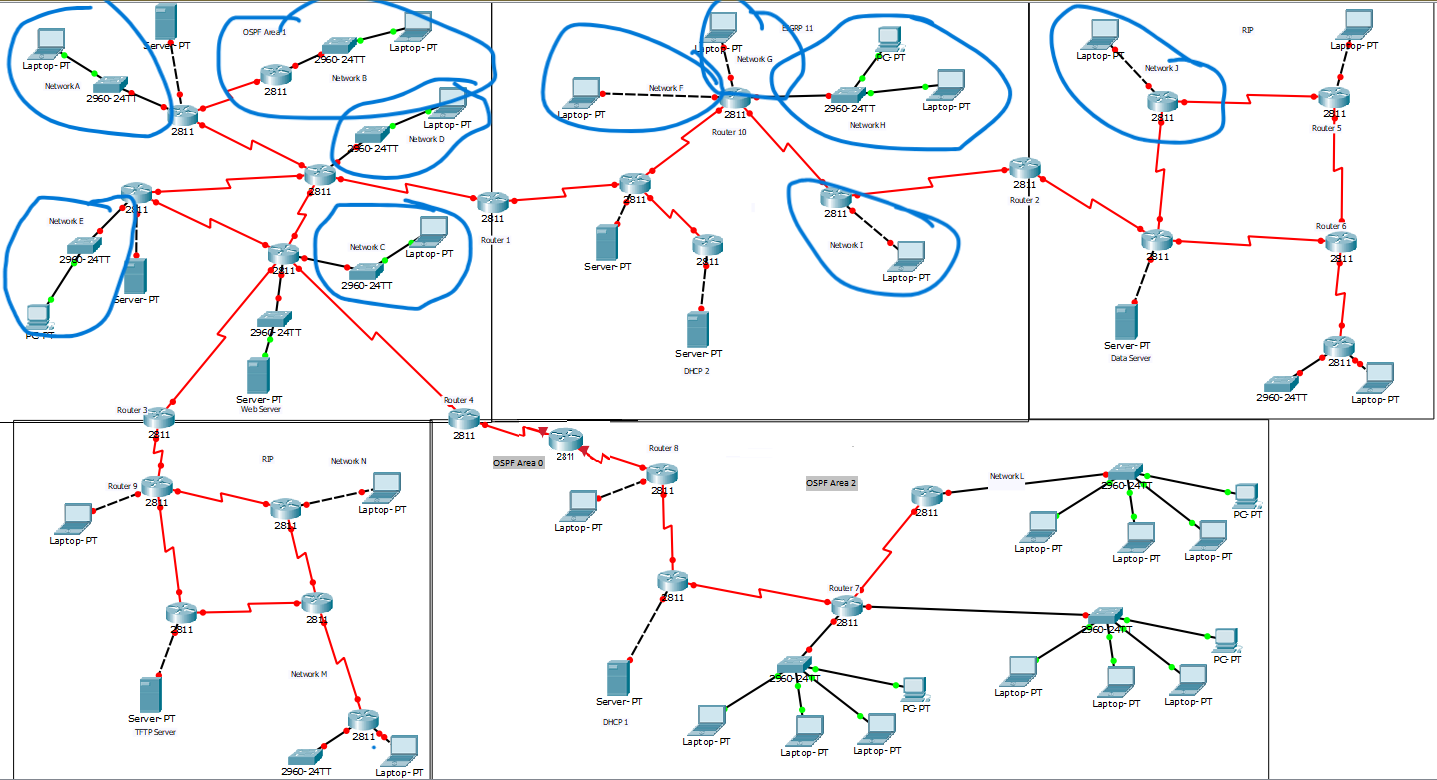
\includegraphics[width=0.3\textwidth]{Project Topology.png}
    \end{center}
    
    \vspace{2cm}
    
    {\Large\bfseries FAST National University}\\[0.5cm]
    {\large\bfseries Computing and Emerging Sciences}\\[0.5cm]
    {\large\bfseries Islamabad Campus}\\[2cm]
    
    \begin{flushleft}
        \large
        \textbf{Student Information:}\\[0.5cm]
        Name: Muhammad Nouman Hafeez\\[0.3cm]
        Roll Number: 21I-0416\\[0.3cm]
        Course: Computer Networks\\[0.3cm]
        Course Semester Project\\[0.3cm]
        Submitted to: Sir Hamza Mehmood\\[0.3cm]
        Date of Submission: 7th December, 2025
    \end{flushleft}
    
    \vfill
    
    {\large \today}
    
\end{titlepage}

% Table of Contents
\tableofcontents
\newpage
\listoffigures
\newpage
\listoftables
\newpage

% Abstract
\chapter*{Abstract}
\addcontentsline{toc}{chapter}{Abstract}

This report presents a comprehensive enterprise network design project implementing Variable Length Subnet Masking (VLSM), multiple routing protocols (RIP, OSPF, EIGRP), DHCP configuration, Access Control Lists (ACLs), Network Address Translation (NAT), and server services. The project successfully allocates IP addresses for 13 primary networks (A through N) with varying host requirements ranging from 835 to 83,492 hosts, along with 29 point-to-point router links and 15 LAN segments, all within a single supernet (114.192.0.0/14). The implementation demonstrates efficient address utilization with 75.6\% usable addresses and includes a comprehensive web-based visualization system for network topology and configuration results.

\newpage

% Chapter 1: Introduction
\chapter{Introduction}

\section{Project Overview}

This project involves the design and implementation of a large-scale enterprise network topology using advanced networking concepts including VLSM subnetting, dynamic routing protocols, and network services. The network accommodates diverse host requirements across multiple subnets while maintaining efficient address space utilization.

\section{Objectives}

The main objectives of this project are:

\begin{itemize}
    \item Design and implement VLSM subnetting for 13 primary networks with varying host requirements
    \item Configure multiple routing protocols (RIP, OSPF, EIGRP) with proper redistribution
    \item Implement DHCP services for automatic IP address allocation
    \item Configure Access Control Lists (ACLs) for network security
    \item Implement Network Address Translation (NAT) for internet connectivity
    \item Configure server services (TFTP, Web, Data servers)
    \item Create an interactive web-based visualization system
\end{itemize}

\section{Network Information}

\begin{itemize}
    \item \textbf{Public IP Address:} 114.192.168.19/24
    \item \textbf{Private IP Address:} 192.168.1.6
    \item \textbf{Supernet:} 114.192.0.0/14 (covers 114.192.0.0 $\rightarrow$ 114.195.255.255)
    \item \textbf{Total Address Space:} 262,144 addresses
\end{itemize}

\section{Project Structure}

This report is organized as follows:

\begin{itemize}
    \item Chapter 2: VLSM Subnetting Configuration
    \item Chapter 3: Routing Protocol Configuration
    \item Chapter 4: DHCP Configuration
    \item Chapter 5: Access Control Lists (ACLs)
    \item Chapter 6: Network Address Translation (NAT)
    \item Chapter 7: Server Services Configuration
    \item Chapter 8: Web-Based Visualization System
    \item Chapter 9: Results and Analysis
    \item Chapter 10: Conclusion
\end{itemize}

\newpage

% Chapter 2: VLSM Configuration
\chapter{VLSM Subnetting Configuration}

\section{Overview}

Variable Length Subnet Masking (VLSM) allows for efficient IP address allocation by using different subnet masks for different subnets within the same network. This approach minimizes address wastage and maximizes address space utilization.

\section{Host Requirements}

The network topology requires 13 primary networks (labeled A through N) with varying host requirements. Table~\ref{tab:host-requirements} shows the original host requirements for each network.

\begin{table}[H]
\centering
\caption{Original Host Requirements}
\label{tab:host-requirements}
\begin{tabular}{@{}cc@{}}
\toprule
\textbf{Network} & \textbf{Required Hosts} \\
\midrule
A & 10,921 \\
B & 14,068 \\
C & 11,243 \\
D & 2,154 \\
E & 7,579 \\
F & 83,492 \\
G & 3,447 \\
H & 851 \\
I & 835 \\
J & 874 \\
L & 8,644 \\
M & 6,021 \\
N & 849 \\
\bottomrule
\end{tabular}
\end{table}

\section{Allocation Strategy}

The allocation strategy follows these principles:

\begin{itemize}
    \item \textbf{Supernet:} 114.192.0.0/14 (covers 114.192.0.0 $\rightarrow$ 114.195.255.255)
    \item \textbf{Allocation Order:} Largest to smallest (minimizes fragmentation)
    \item \textbf{Algorithm:} For each required hosts $R$, choose the smallest $H$ where $2^H - 2 \geq R$, then prefix $= 32 - H$
\end{itemize}

Table~\ref{tab:sorted-requirements} shows the sorted host requirements in descending order.

\begin{table}[H]
\centering
\caption{Sorted Host Requirements (Max $\rightarrow$ Min)}
\label{tab:sorted-requirements}
\begin{tabular}{@{}cc@{}}
\toprule
\textbf{Network} & \textbf{Required Hosts} \\
\midrule
F & 83,492 \\
B & 14,068 \\
C & 11,243 \\
A & 10,921 \\
L & 8,644 \\
E & 7,579 \\
M & 6,021 \\
G & 3,447 \\
D & 2,154 \\
J & 874 \\
H & 851 \\
N & 849 \\
I & 835 \\
\bottomrule
\end{tabular}
\end{table}

\section{Detailed Network Allocations}

\subsection{Network F (Largest Network)}

\begin{itemize}
    \item \textbf{Required:} 83,492 hosts
    \item \textbf{H Calculation:} $2^{16} - 2 = 65,534$ (too small), $2^{17} - 2 = 131,070$ (OK) $\rightarrow H = 17$
    \item \textbf{Prefix:} /15
    \item \textbf{Subnet Mask:} 255.254.0.0
    \item \textbf{Total Addresses:} $2^{17} = 131,072$
    \item \textbf{Usable Addresses:} $2^{17} - 2 = 131,070$
    \item \textbf{Waste:} 47,578 (36.3\%)
    \item \textbf{Assigned Network:} 114.192.0.0/15
    \item \textbf{First Usable:} 114.192.0.1
    \item \textbf{Last Usable:} 114.193.255.254
    \item \textbf{Broadcast:} 114.193.255.255
\end{itemize}

\subsection{Network B}

\begin{itemize}
    \item \textbf{Required:} 14,068 hosts
    \item \textbf{H Calculation:} $2^{14} - 2 = 16,382 \geq 14,068 \rightarrow H = 14$
    \item \textbf{Prefix:} /18
    \item \textbf{Subnet Mask:} 255.255.192.0
    \item \textbf{Total Addresses:} $2^{14} = 16,384$
    \item \textbf{Usable Addresses:} $2^{14} - 2 = 16,382$
    \item \textbf{Waste:} 2,314 (14.1\%)
    \item \textbf{Assigned Network:} 114.194.0.0/18
    \item \textbf{First Usable:} 114.194.0.1
    \item \textbf{Last Usable:} 114.194.63.254
    \item \textbf{Broadcast:} 114.194.63.255
\end{itemize}

\subsection{Network C}

\begin{itemize}
    \item \textbf{Required:} 11,243 hosts
    \item \textbf{Prefix:} /18
    \item \textbf{Subnet Mask:} 255.255.192.0
    \item \textbf{Usable Addresses:} 16,382
    \item \textbf{Waste:} 5,139 (31.4\%)
    \item \textbf{Assigned Network:} 114.194.64.0/18
    \item \textbf{First Usable:} 114.194.64.1
    \item \textbf{Last Usable:} 114.194.127.254
    \item \textbf{Broadcast:} 114.194.127.255
\end{itemize}

\subsection{Network A}

\begin{itemize}
    \item \textbf{Required:} 10,921 hosts
    \item \textbf{Prefix:} /18
    \item \textbf{Subnet Mask:} 255.255.192.0
    \item \textbf{Usable Addresses:} 16,382
    \item \textbf{Waste:} 5,461 (33.3\%)
    \item \textbf{Assigned Network:} 114.194.128.0/18
    \item \textbf{First Usable:} 114.194.128.1
    \item \textbf{Last Usable:} 114.194.191.254
    \item \textbf{Broadcast:} 114.194.191.255
\end{itemize}

\subsection{Network L}

\begin{itemize}
    \item \textbf{Required:} 8,644 hosts
    \item \textbf{Prefix:} /18
    \item \textbf{Subnet Mask:} 255.255.192.0
    \item \textbf{Usable Addresses:} 16,382
    \item \textbf{Waste:} 7,738 (47.2\%)
    \item \textbf{Assigned Network:} 114.194.192.0/18
    \item \textbf{First Usable:} 114.194.192.1
    \item \textbf{Last Usable:} 114.194.255.254
    \item \textbf{Broadcast:} 114.194.255.255
\end{itemize}

\subsection{Network E}

\begin{itemize}
    \item \textbf{Required:} 7,579 hosts
    \item \textbf{H Calculation:} $2^{13} - 2 = 8,190 \geq 7,579 \rightarrow H = 13$
    \item \textbf{Prefix:} /19
    \item \textbf{Subnet Mask:} 255.255.224.0
    \item \textbf{Total Addresses:} $2^{13} = 8,192$
    \item \textbf{Usable Addresses:} $2^{13} - 2 = 8,190$
    \item \textbf{Waste:} 611 (7.5\%)
    \item \textbf{Assigned Network:} 114.195.0.0/19
    \item \textbf{First Usable:} 114.195.0.1
    \item \textbf{Last Usable:} 114.195.31.254
    \item \textbf{Broadcast:} 114.195.31.255
\end{itemize}

\subsection{Network M}

\begin{itemize}
    \item \textbf{Required:} 6,021 hosts
    \item \textbf{Prefix:} /19
    \item \textbf{Subnet Mask:} 255.255.224.0
    \item \textbf{Usable Addresses:} 8,190
    \item \textbf{Waste:} 2,169 (26.5\%)
    \item \textbf{Assigned Network:} 114.195.32.0/19
    \item \textbf{First Usable:} 114.195.32.1
    \item \textbf{Last Usable:} 114.195.63.254
    \item \textbf{Broadcast:} 114.195.63.255
\end{itemize}

\subsection{Network G}

\begin{itemize}
    \item \textbf{Required:} 3,447 hosts
    \item \textbf{H Calculation:} $2^{12} - 2 = 4,094 \geq 3,447 \rightarrow H = 12$
    \item \textbf{Prefix:} /20
    \item \textbf{Subnet Mask:} 255.255.240.0
    \item \textbf{Total Addresses:} $2^{12} = 4,096$
    \item \textbf{Usable Addresses:} $2^{12} - 2 = 4,094$
    \item \textbf{Waste:} 647 (15.8\%)
    \item \textbf{Assigned Network:} 114.195.64.0/20
    \item \textbf{First Usable:} 114.195.64.1
    \item \textbf{Last Usable:} 114.195.79.254
    \item \textbf{Broadcast:} 114.195.79.255
\end{itemize}

\subsection{Network D}

\begin{itemize}
    \item \textbf{Required:} 2,154 hosts
    \item \textbf{Prefix:} /20
    \item \textbf{Subnet Mask:} 255.255.240.0
    \item \textbf{Usable Addresses:} 4,094
    \item \textbf{Waste:} 1,940 (47.4\%)
    \item \textbf{Assigned Network:} 114.195.80.0/20
    \item \textbf{First Usable:} 114.195.80.1
    \item \textbf{Last Usable:} 114.195.95.254
    \item \textbf{Broadcast:} 114.195.95.255
\end{itemize}

\subsection{Network J}

\begin{itemize}
    \item \textbf{Required:} 874 hosts
    \item \textbf{H Calculation:} $2^{10} - 2 = 1,022 \geq 874 \rightarrow H = 10$
    \item \textbf{Prefix:} /22
    \item \textbf{Subnet Mask:} 255.255.252.0
    \item \textbf{Total Addresses:} $2^{10} = 1,024$
    \item \textbf{Usable Addresses:} $2^{10} - 2 = 1,022$
    \item \textbf{Waste:} 148 (14.5\%)
    \item \textbf{Assigned Network:} 114.195.96.0/22
    \item \textbf{First Usable:} 114.195.96.1
    \item \textbf{Last Usable:} 114.195.99.254
    \item \textbf{Broadcast:} 114.195.99.255
\end{itemize}

\subsection{Network H}

\begin{itemize}
    \item \textbf{Required:} 851 hosts
    \item \textbf{Prefix:} /22
    \item \textbf{Subnet Mask:} 255.255.252.0
    \item \textbf{Usable Addresses:} 1,022
    \item \textbf{Waste:} 171 (16.7\%)
    \item \textbf{Assigned Network:} 114.195.100.0/22
    \item \textbf{First Usable:} 114.195.100.1
    \item \textbf{Last Usable:} 114.195.103.254
    \item \textbf{Broadcast:} 114.195.103.255
\end{itemize}

\subsection{Network N}

\begin{itemize}
    \item \textbf{Required:} 849 hosts
    \item \textbf{Prefix:} /22
    \item \textbf{Subnet Mask:} 255.255.252.0
    \item \textbf{Usable Addresses:} 1,022
    \item \textbf{Waste:} 173 (16.9\%)
    \item \textbf{Assigned Network:} 114.195.104.0/22
    \item \textbf{First Usable:} 114.195.104.1
    \item \textbf{Last Usable:} 114.195.107.254
    \item \textbf{Broadcast:} 114.195.107.255
\end{itemize}

\subsection{Network I (Smallest Network)}

\begin{itemize}
    \item \textbf{Required:} 835 hosts
    \item \textbf{Prefix:} /22
    \item \textbf{Subnet Mask:} 255.255.252.0
    \item \textbf{Usable Addresses:} 1,022
    \item \textbf{Waste:} 187 (18.3\%)
    \item \textbf{Assigned Network:} 114.195.108.0/22
    \item \textbf{First Usable:} 114.195.108.1
    \item \textbf{Last Usable:} 114.195.111.254
    \item \textbf{Broadcast:} 114.195.111.255
\end{itemize}

\section{Complete VLSM Allocation Summary}

Table~\ref{tab:vlsm-summary} provides a complete summary of all network allocations.

\begin{longtable}{@{}p{1.5cm}p{2cm}p{1.5cm}p{2.5cm}p{2cm}p{2cm}p{2cm}@{}}
\caption{Complete VLSM Allocation Summary}
\label{tab:vlsm-summary}
\\ \toprule
\textbf{Net} & \textbf{Subnet} & \textbf{Prefix} & \textbf{Subnet Mask} & \textbf{First Usable} & \textbf{Last Usable} & \textbf{Broadcast} \\
\midrule
\endfirsthead
\multicolumn{7}{c}{{\bfseries \tablename\ \thetable{} -- continued from previous page}} \\
\toprule
\textbf{Net} & \textbf{Subnet} & \textbf{Prefix} & \textbf{Subnet Mask} & \textbf{First Usable} & \textbf{Last Usable} & \textbf{Broadcast} \\
\midrule
\endhead
\bottomrule
\endfoot
\bottomrule
\endlastfoot
F & 114.192.0.0/15 & /15 & 255.254.0.0 & 114.192.0.1 & 114.193.255.254 & 114.193.255.255 \\
B & 114.194.0.0/18 & /18 & 255.255.192.0 & 114.194.0.1 & 114.194.63.254 & 114.194.63.255 \\
C & 114.194.64.0/18 & /18 & 255.255.192.0 & 114.194.64.1 & 114.194.127.254 & 114.194.127.255 \\
A & 114.194.128.0/18 & /18 & 255.255.192.0 & 114.194.128.1 & 114.194.191.254 & 114.194.191.255 \\
L & 114.194.192.0/18 & /18 & 255.255.192.0 & 114.194.192.1 & 114.194.255.254 & 114.194.255.255 \\
E & 114.195.0.0/19 & /19 & 255.255.224.0 & 114.195.0.1 & 114.195.31.254 & 114.195.31.255 \\
M & 114.195.32.0/19 & /19 & 255.255.224.0 & 114.195.32.1 & 114.195.63.254 & 114.195.63.255 \\
G & 114.195.64.0/20 & /20 & 255.255.240.0 & 114.195.64.1 & 114.195.79.254 & 114.195.79.255 \\
D & 114.195.80.0/20 & /20 & 255.255.240.0 & 114.195.80.1 & 114.195.95.254 & 114.195.95.255 \\
J & 114.195.96.0/22 & /22 & 255.255.252.0 & 114.195.96.1 & 114.195.99.254 & 114.195.99.255 \\
H & 114.195.100.0/22 & /22 & 255.255.252.0 & 114.195.100.1 & 114.195.103.254 & 114.195.103.255 \\
N & 114.195.104.0/22 & /22 & 255.255.252.0 & 114.195.104.1 & 114.195.107.254 & 114.195.107.255 \\
I & 114.195.108.0/22 & /22 & 255.255.252.0 & 114.195.108.1 & 114.195.111.254 & 114.195.111.255 \\
\end{longtable}

\section{VLSM Tree Visualizations}

Figure~\ref{fig:vlsm-tree-1} and Figure~\ref{fig:vlsm-tree-2} show the VLSM subnetting tree visualizations for the primary networks.

\begin{figure}[H]
    \centering
    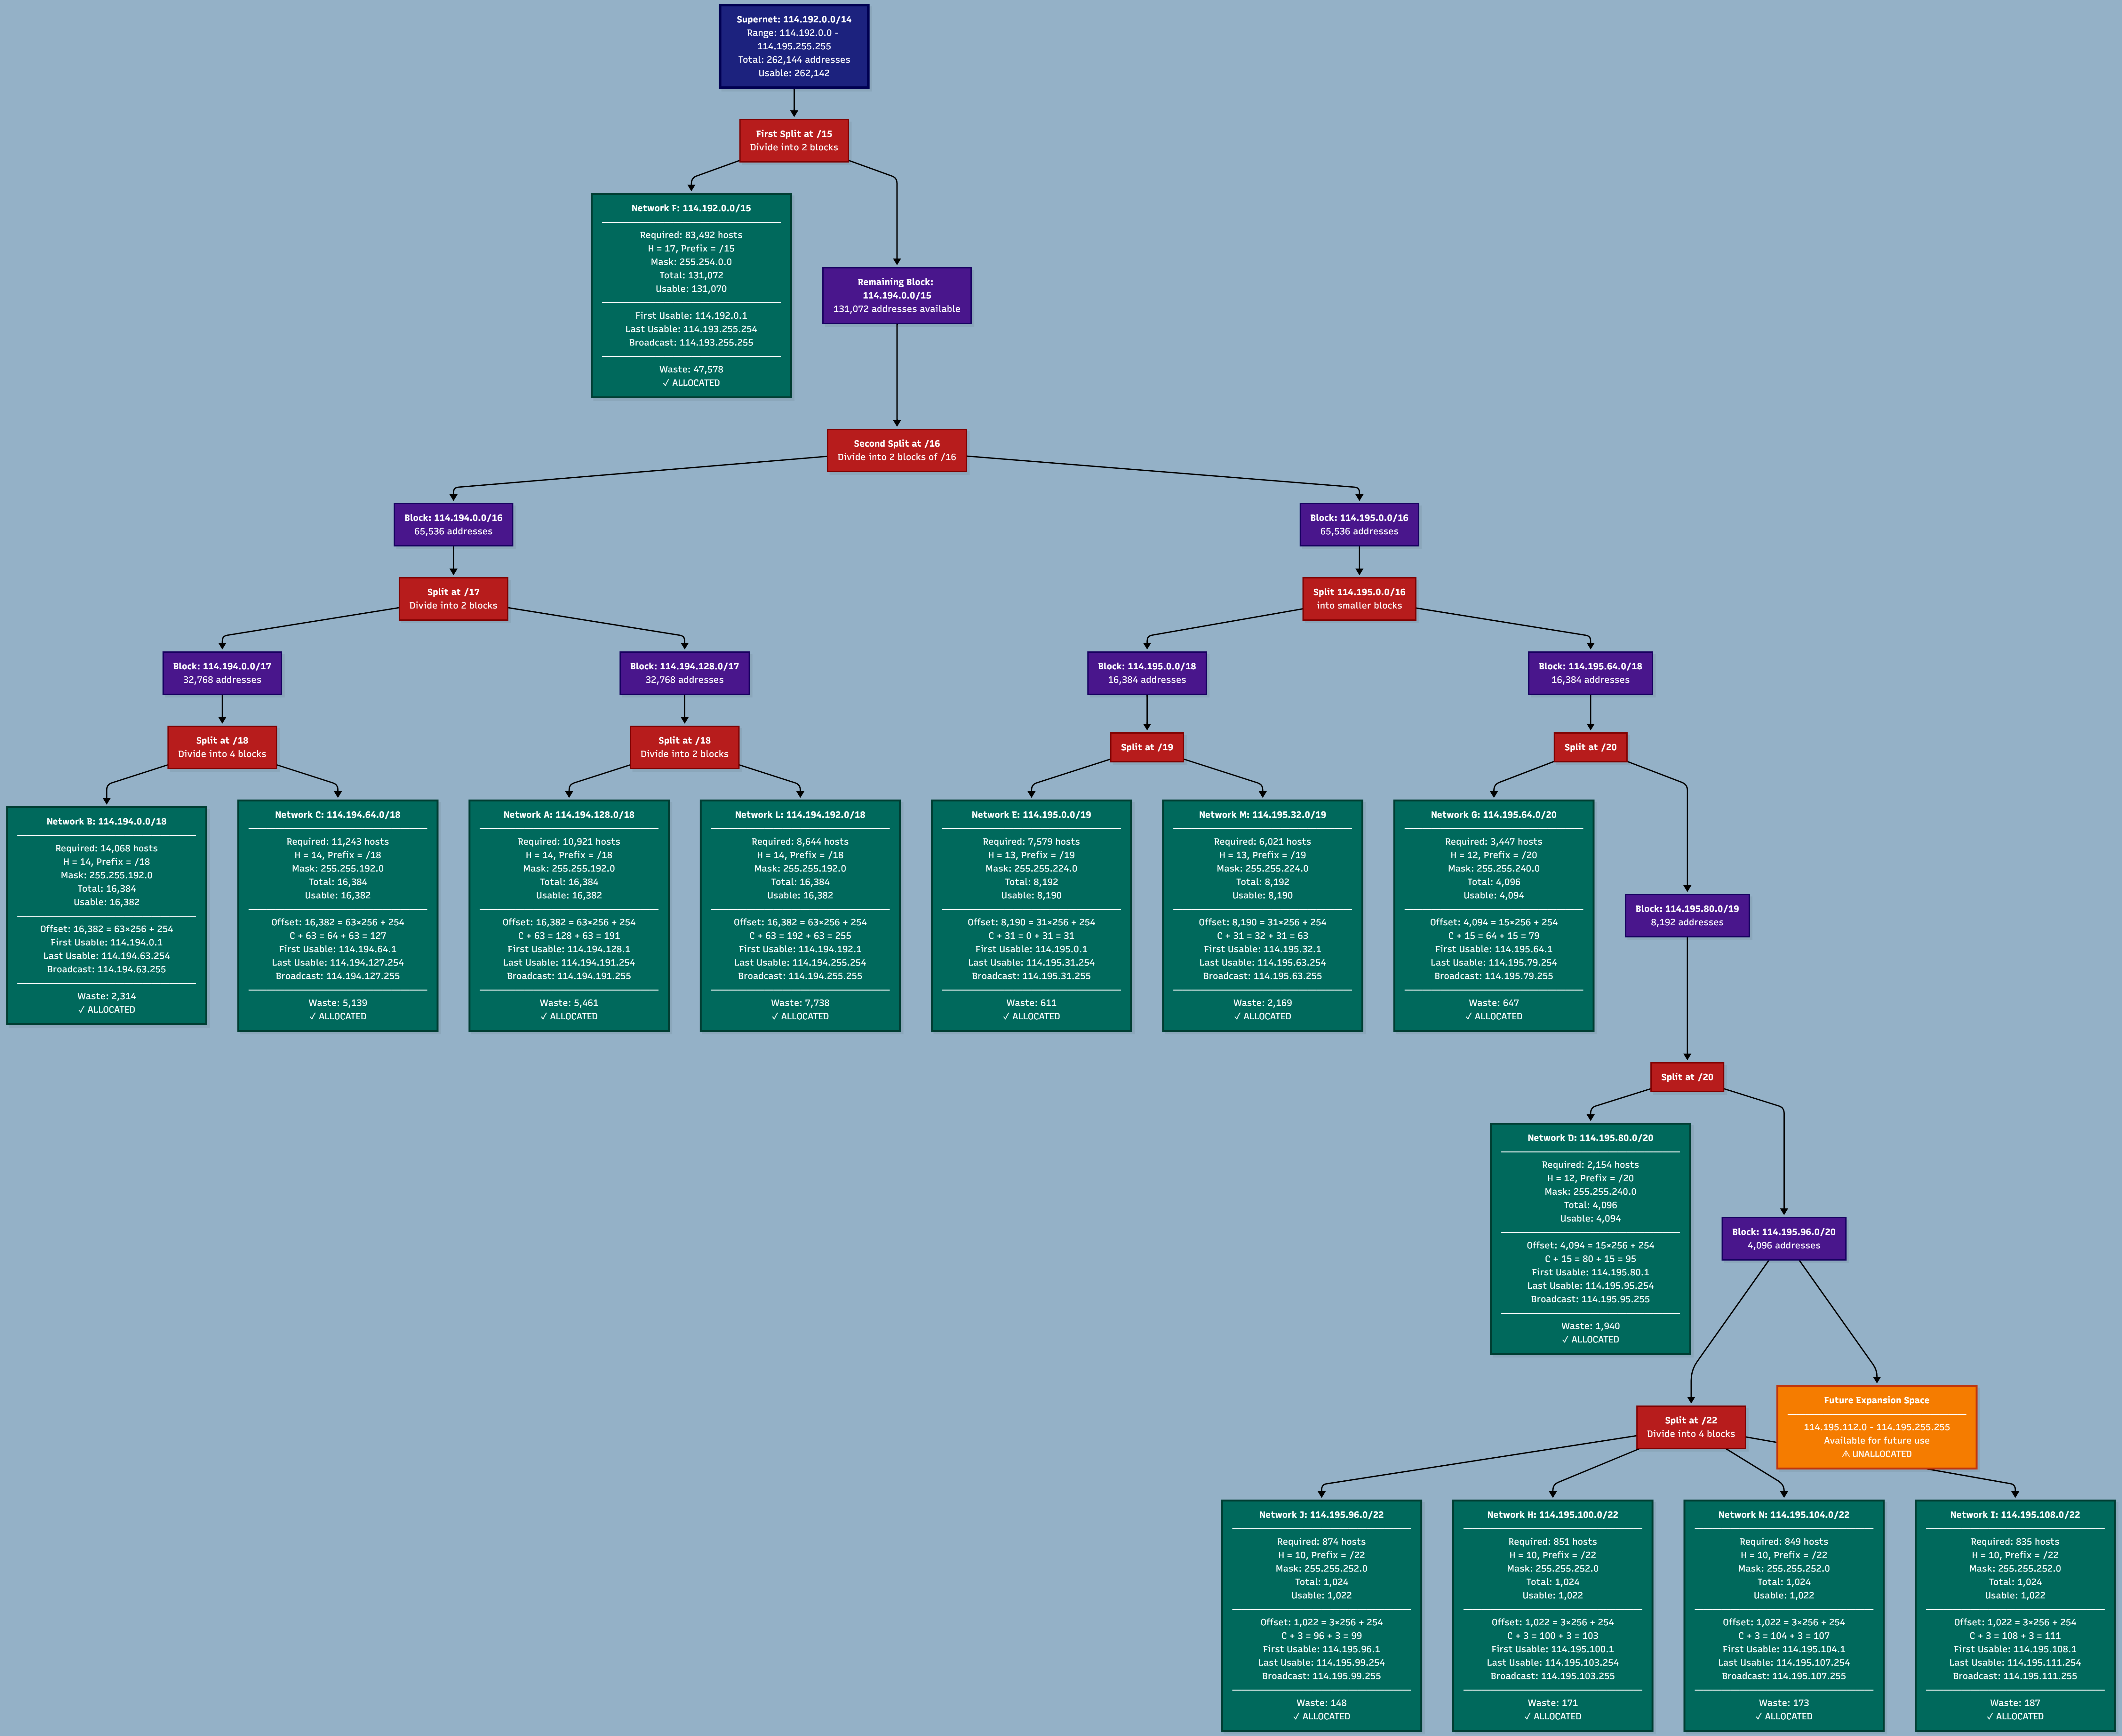
\includegraphics[width=0.9\textwidth]{VLSM-tree-1.png}
    \caption{VLSM Tree Visualization - Part 1}
    \label{fig:vlsm-tree-1}
\end{figure}

\begin{figure}[H]
    \centering
    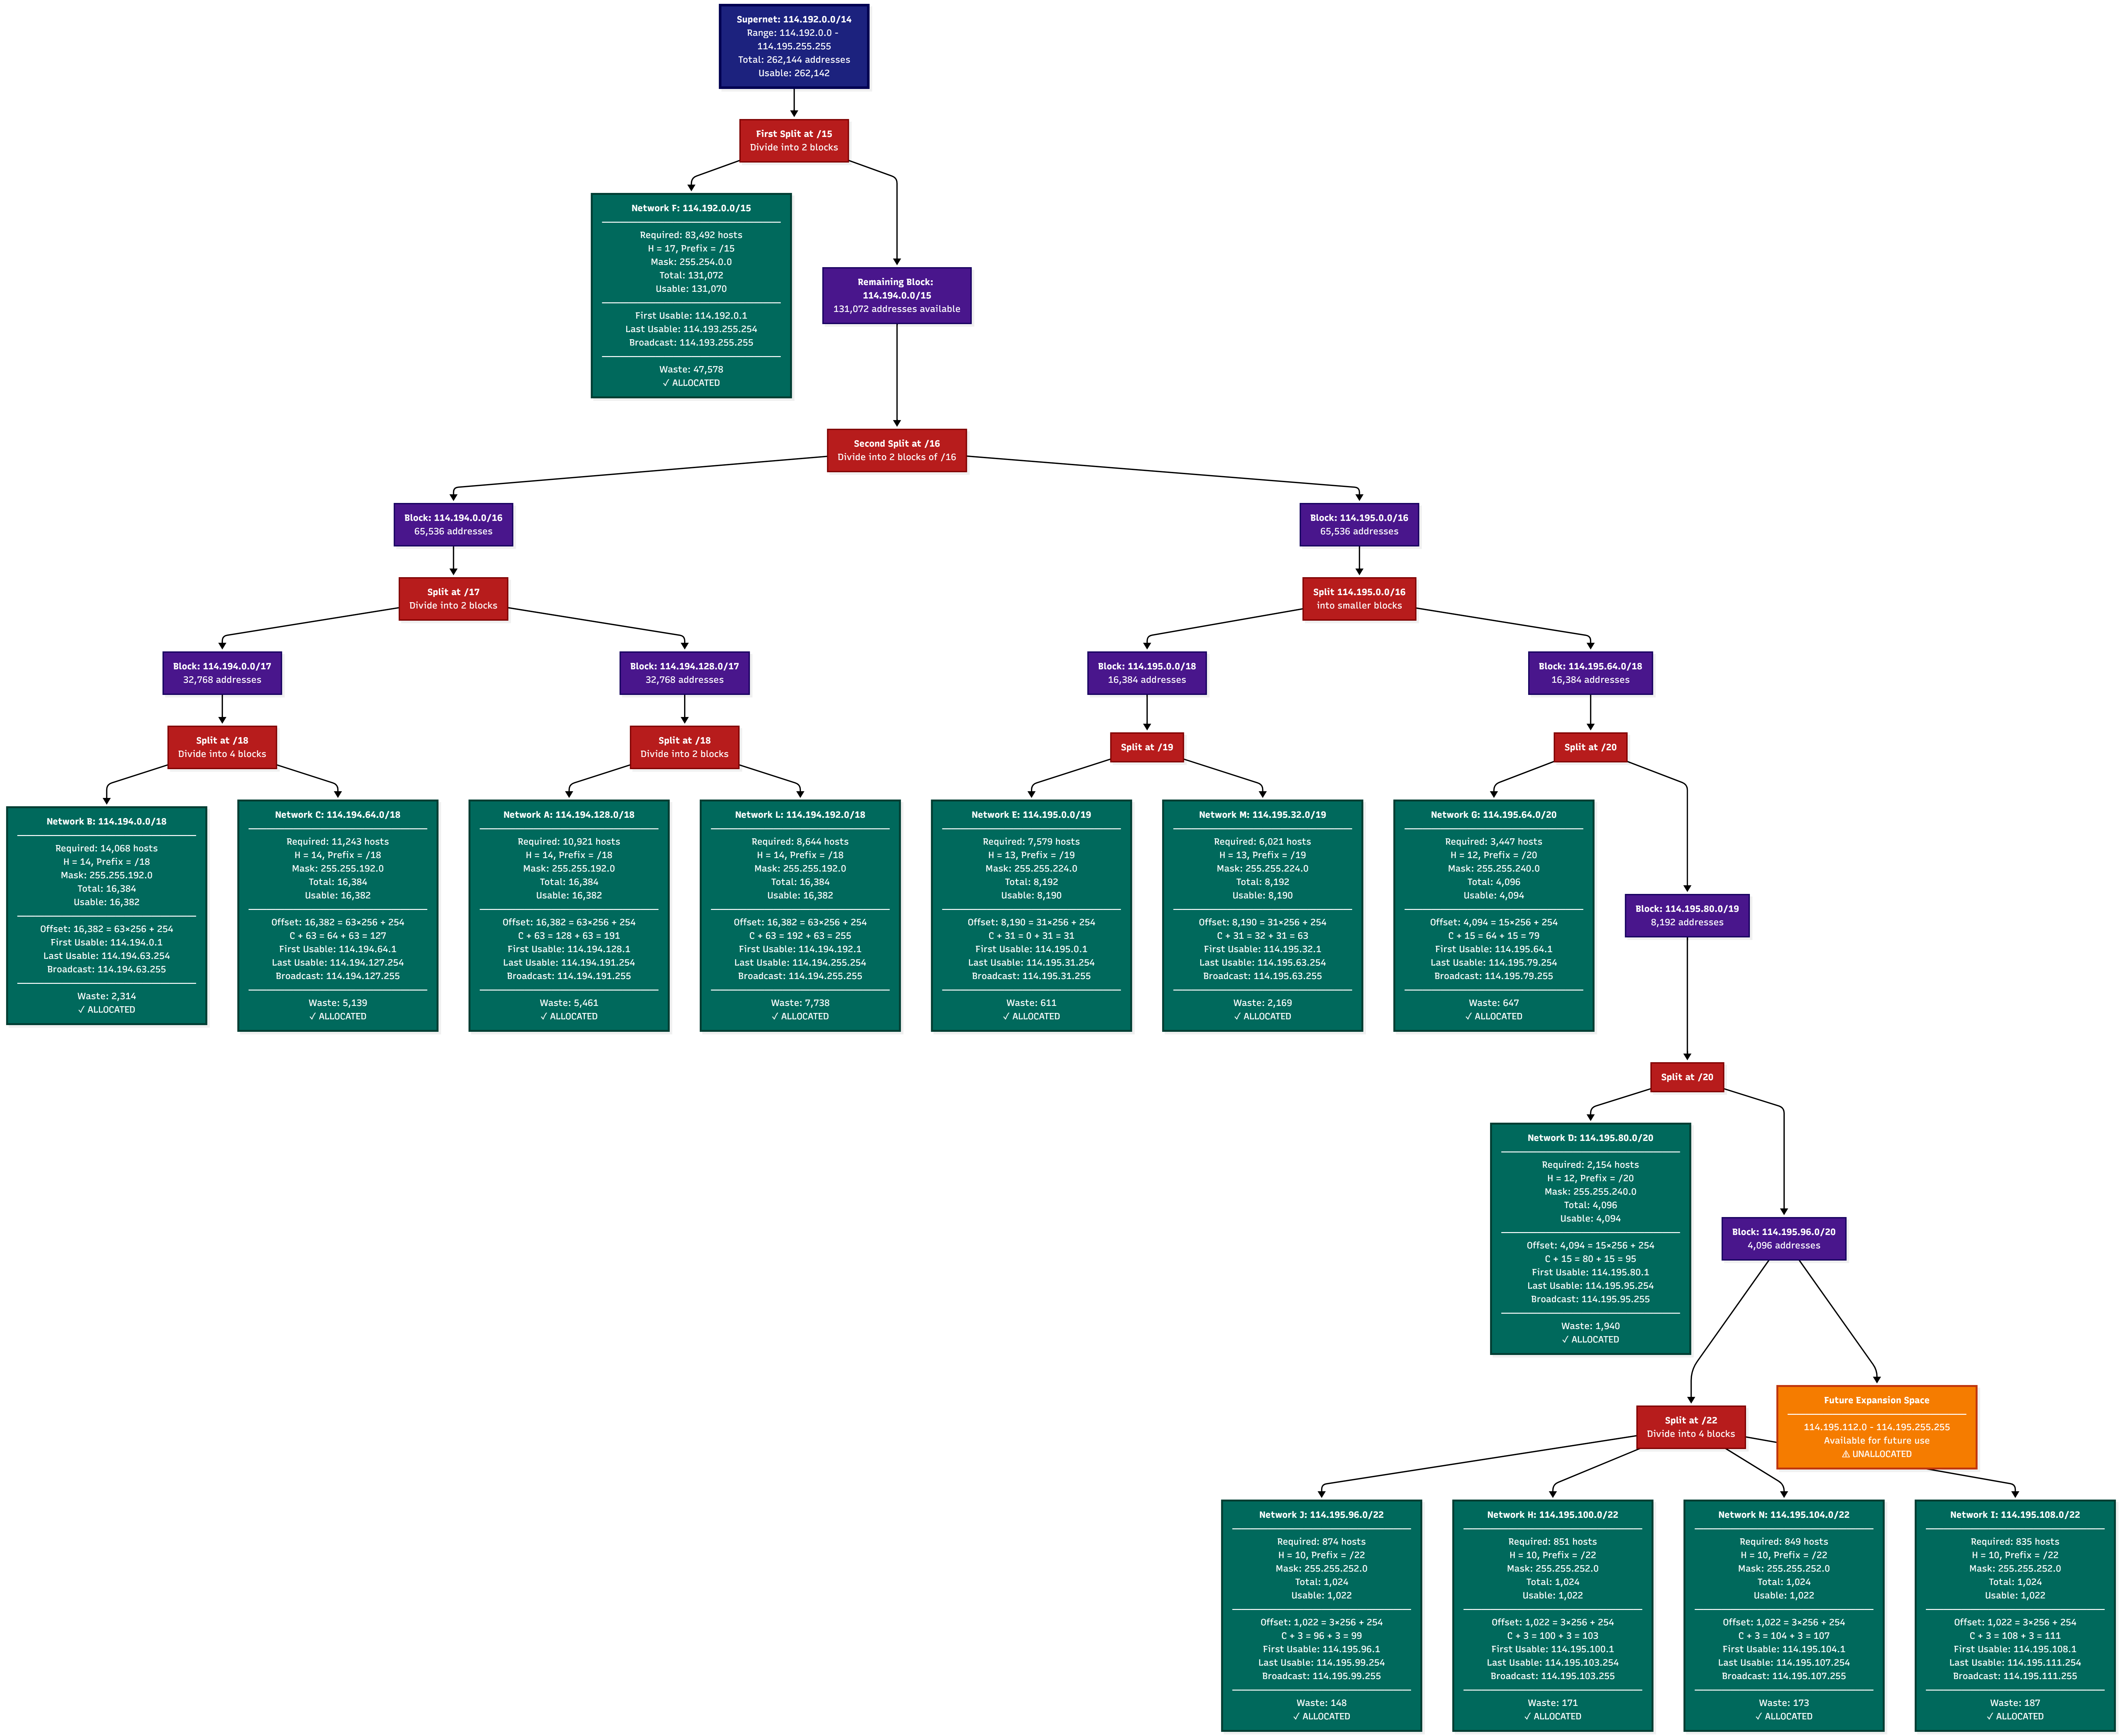
\includegraphics[width=0.9\textwidth]{VLSM-tree-2.png}
    \caption{VLSM Tree Visualization - Part 2}
    \label{fig:vlsm-tree-2}
\end{figure}

\section{Additional Network Allocations}

Beyond the 13 primary networks, the topology requires additional subnetting for inter-router communication links and LAN segments.

\subsection{Point-to-Point Router Links}

The network requires 29 point-to-point router links, each using a /30 subnet mask:

\begin{itemize}
    \item \textbf{Prefix:} /30
    \item \textbf{Subnet Mask:} 255.255.255.252
    \item \textbf{Host Bits:} $H = 2$
    \item \textbf{Total Addresses:} $2^2 = 4$
    \item \textbf{Usable Addresses:} $2^2 - 2 = 2$
    \item \textbf{Total Space Needed:} $29 \times 4 = 116$ addresses
    \item \textbf{Range:} 114.195.112.0 - 114.195.112.115
\end{itemize}

\subsection{LAN Segments}

The network requires 15 small LAN segments, each using a /29 subnet mask:

\begin{itemize}
    \item \textbf{Prefix:} /29
    \item \textbf{Subnet Mask:} 255.255.255.248
    \item \textbf{Host Bits:} $H = 3$
    \item \textbf{Total Addresses:} $2^3 = 8$
    \item \textbf{Usable Addresses:} $2^3 - 2 = 6$
    \item \textbf{Total Space Needed:} $15 \times 8 = 120$ addresses
    \item \textbf{Range:} 114.195.112.120 - 114.195.112.239
\end{itemize}

Figure~\ref{fig:vlsm-other} shows the VLSM tree for additional networks.

\begin{figure}[H]
    \centering
    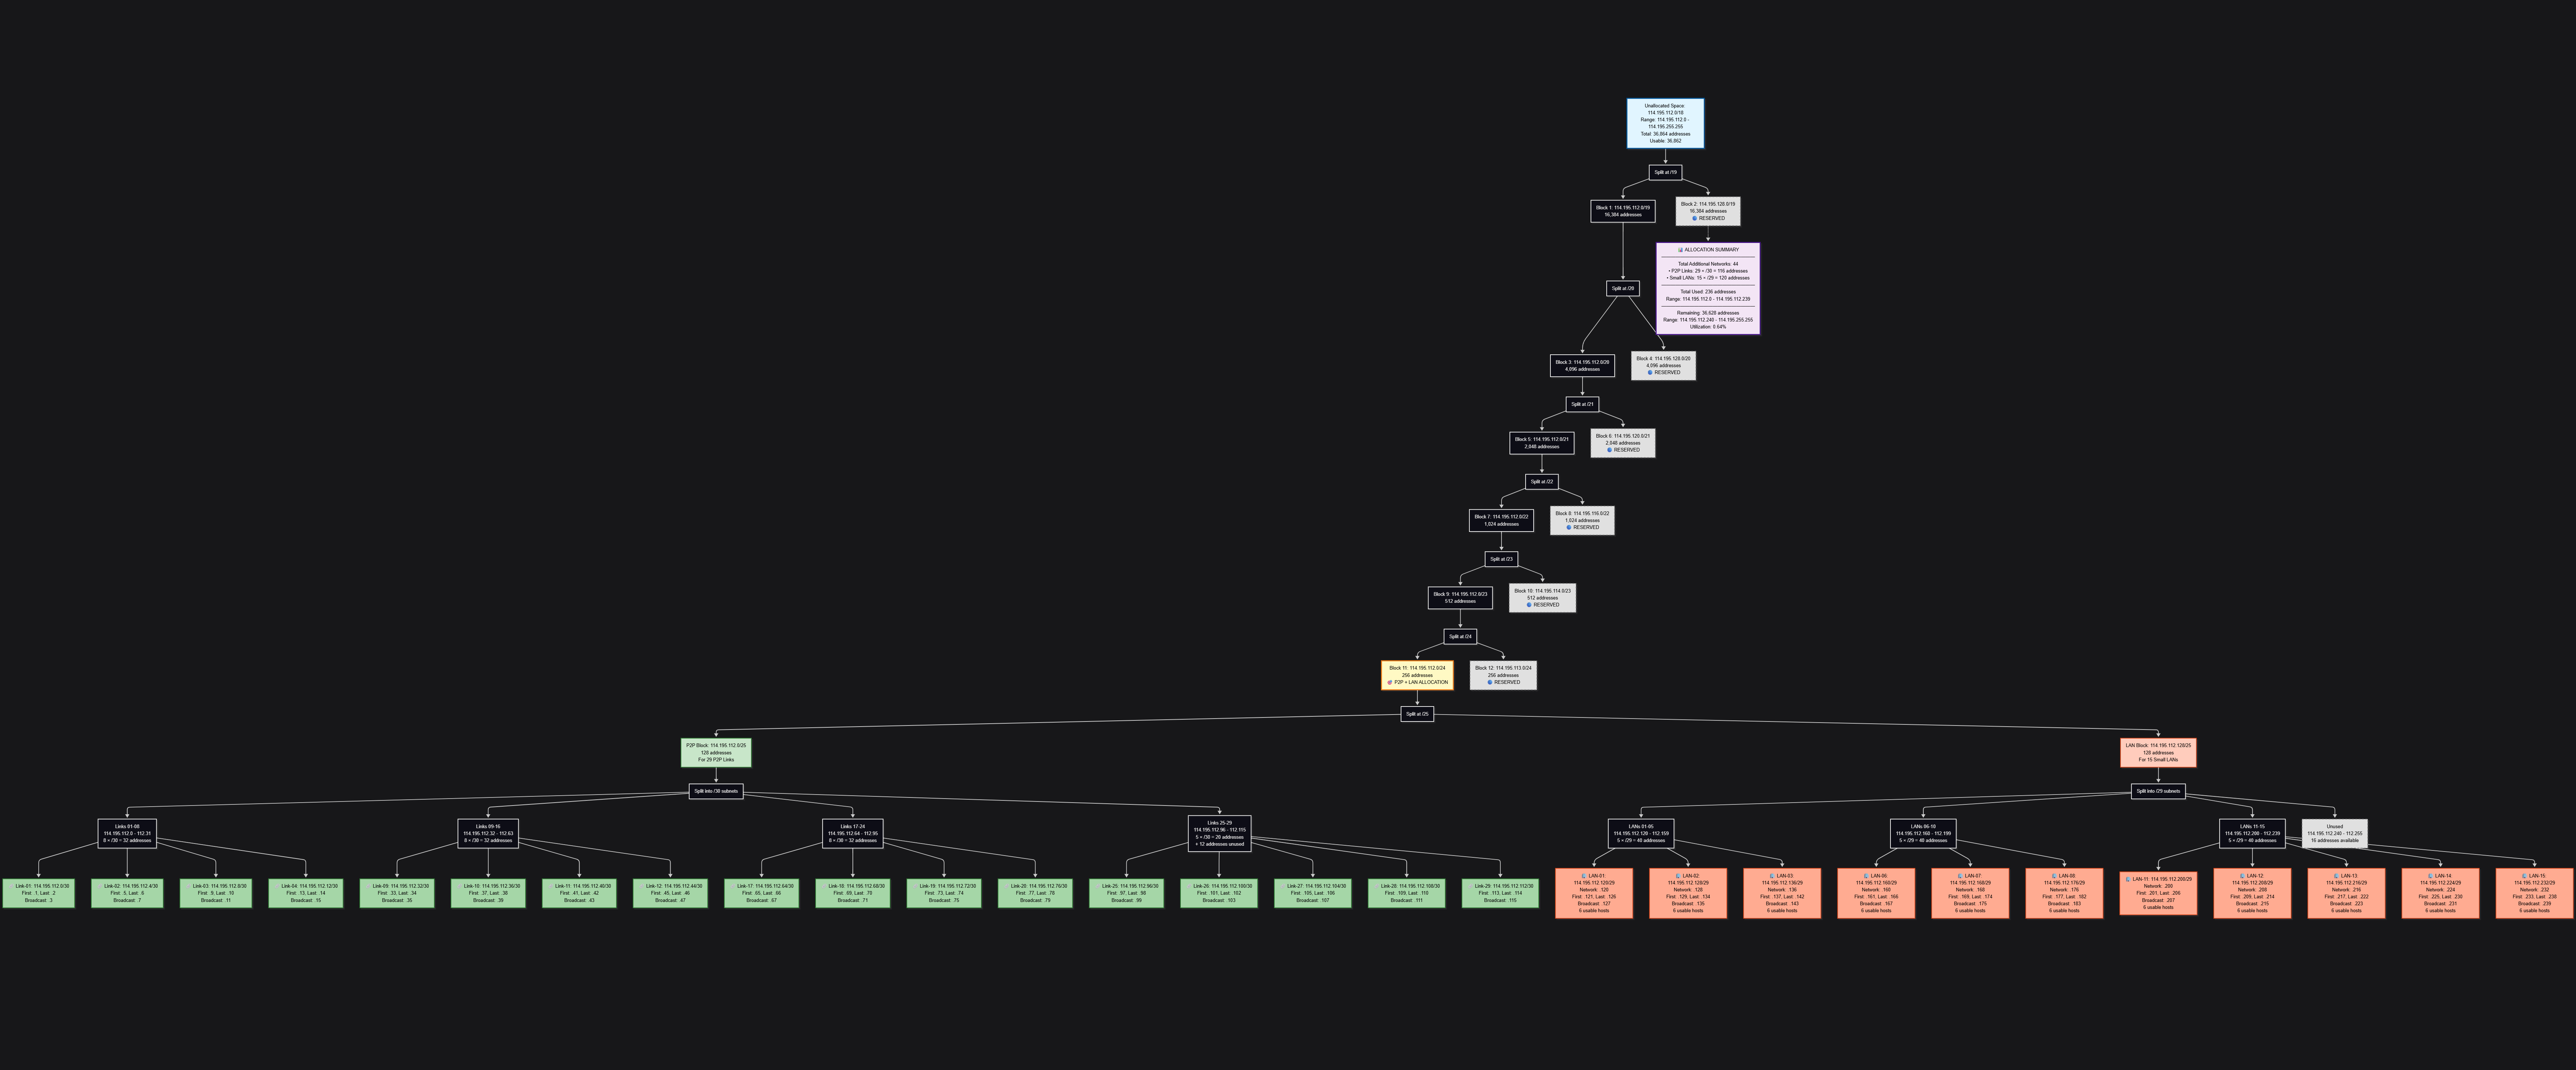
\includegraphics[width=0.9\textwidth]{VLSM-tree-other_networks.png}
    \caption{VLSM Tree for Additional Networks (P2P Links and LAN Segments)}
    \label{fig:vlsm-other}
\end{figure}

\section{Summary Statistics}

Table~\ref{tab:summary-stats} provides summary statistics for the VLSM allocation.

\begin{table}[H]
\centering
\caption{VLSM Summary Statistics}
\label{tab:summary-stats}
\begin{tabular}{@{}lc@{}}
\toprule
\textbf{Metric} & \textbf{Value} \\
\midrule
Total Required Hosts & 150,978 \\
Total Allocated Addresses & 199,680 \\
Total Usable Addresses & 199,652 \\
Total Waste & 48,674 addresses (24.4\%) \\
Supernet Used & 114.192.0.0 to 114.195.111.255 \\
Supernet Range & 114.192.0.0/14 \\
Remaining Space & 114.195.112.0 to 114.195.255.255 \\
\bottomrule
\end{tabular}
\end{table}

\newpage

% Chapter 3: Routing Protocols
\chapter{Routing Protocol Configuration}

This chapter documents the configuration and implementation of three routing protocols: RIP (Routing Information Protocol), OSPF (Open Shortest Path First), and EIGRP (Enhanced Interior Gateway Routing Protocol), along with their redistribution mechanisms.

\section{RIP Configuration}

RIP is a distance-vector routing protocol that uses hop count as its metric. Figure~\ref{fig:rip-commands} shows the RIP configuration commands.

\begin{figure}[H]
    \centering
    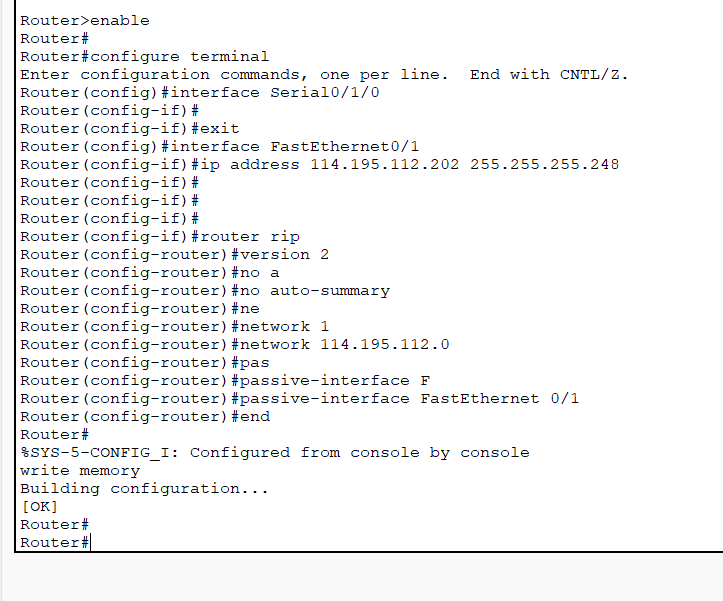
\includegraphics[width=0.9\textwidth]{results/rip_commands.png}
    \caption{RIP Configuration Commands}
    \label{fig:rip-commands}
\end{figure}

Figure~\ref{fig:rip-results} shows RIP routing table results and verification.

\begin{figure}[H]
    \centering
    \begin{subfigure}{0.48\textwidth}
        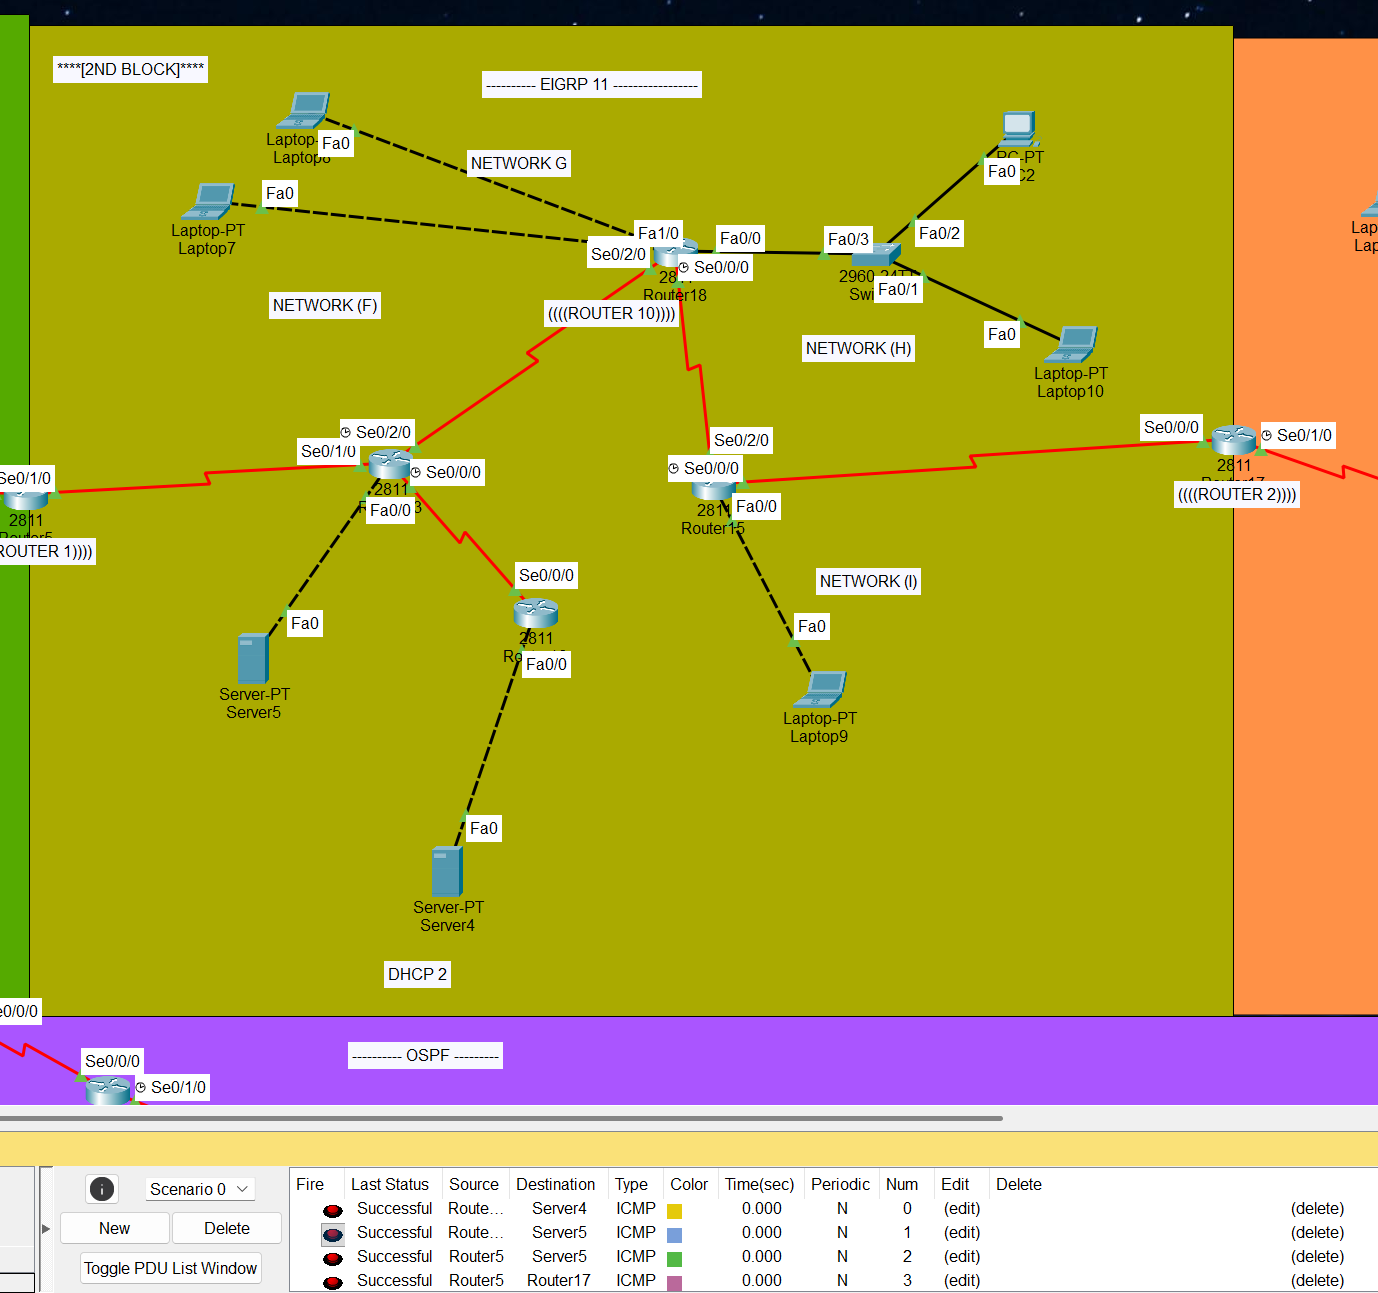
\includegraphics[width=\textwidth]{results/rip_row1_block2_message.png}
        \caption{RIP Row 1 Block 2 Message}
    \end{subfigure}
    \hfill
    \begin{subfigure}{0.48\textwidth}
        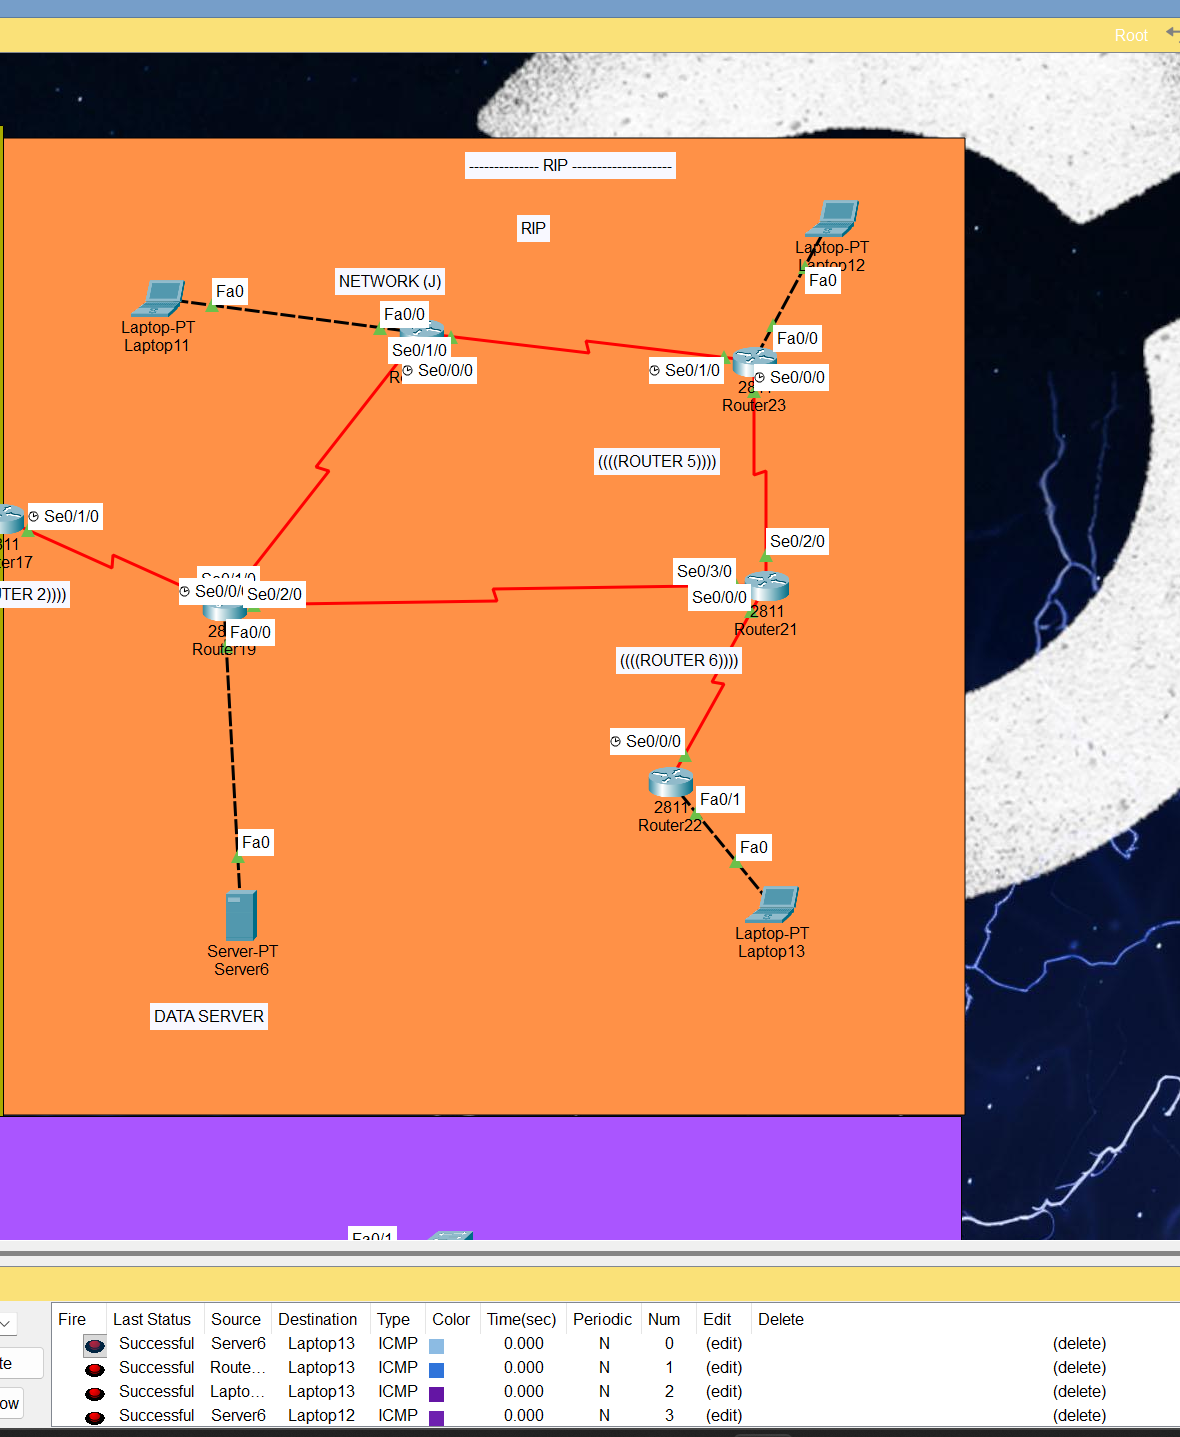
\includegraphics[width=\textwidth]{results/rip_row1_block3_message.png}
        \caption{RIP Row 1 Block 3 Message}
    \end{subfigure}
    \caption{RIP Routing Verification Results}
    \label{fig:rip-results}
\end{figure}

\section{OSPF Configuration}

OSPF is a link-state routing protocol that uses Dijkstra's algorithm. The network is divided into multiple OSPF areas for hierarchical routing.

\subsection{OSPF Area 0 Configuration}

Area 0 serves as the backbone area. Figure~\ref{fig:ospf-area0} shows the Area 0 configuration and verification.

\begin{figure}[H]
    \centering
    \begin{subfigure}{0.48\textwidth}
        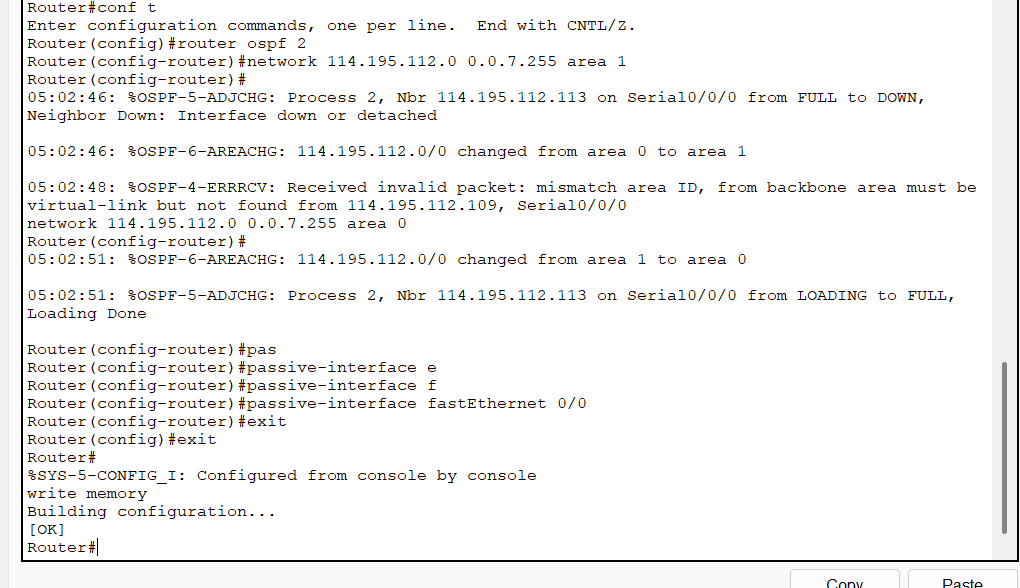
\includegraphics[width=\textwidth]{results/ospf_area0_commands.png}
        \caption{OSPF Area 0 Commands - Part 1}
    \end{subfigure}
    \hfill
    \begin{subfigure}{0.48\textwidth}
        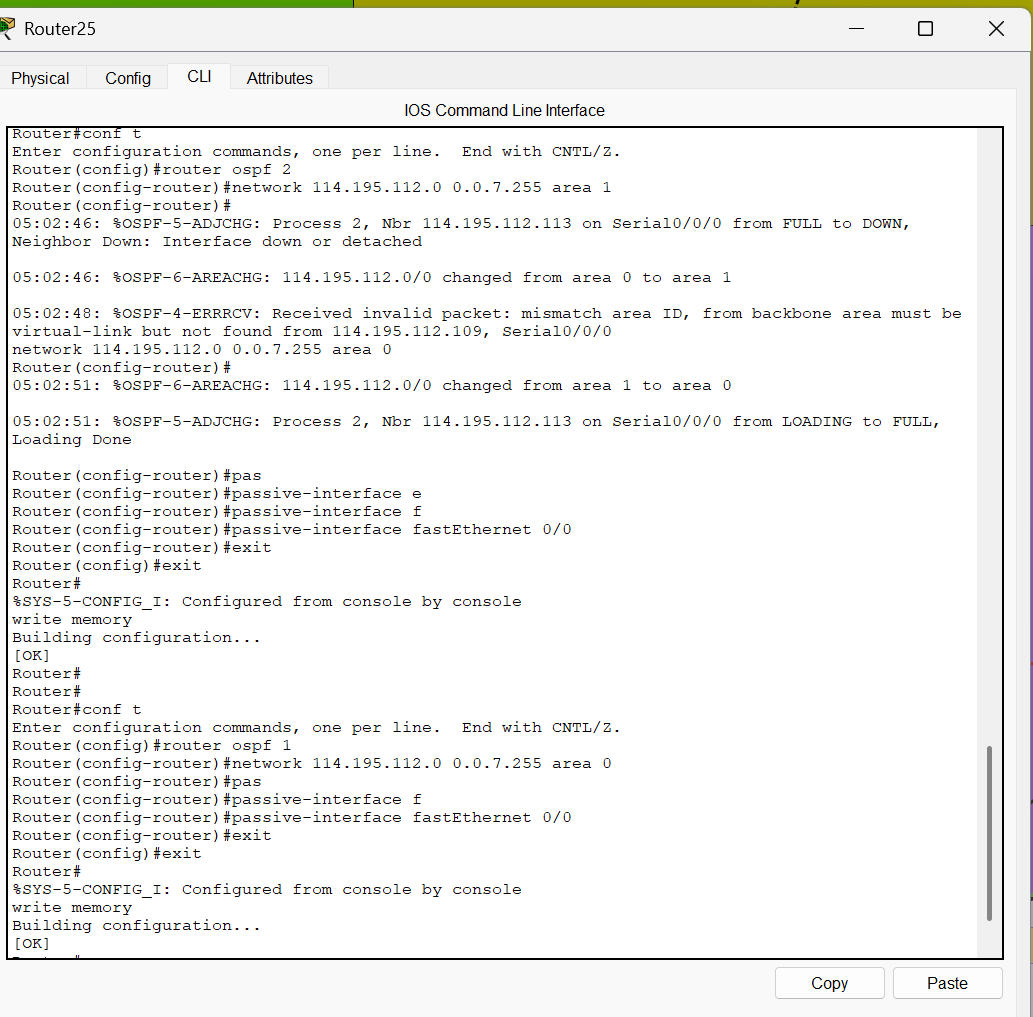
\includegraphics[width=\textwidth]{results/ospf_area0_commands_2.png}
        \caption{OSPF Area 0 Commands - Part 2}
    \end{subfigure}
    \vspace{0.5cm}
    \centering
    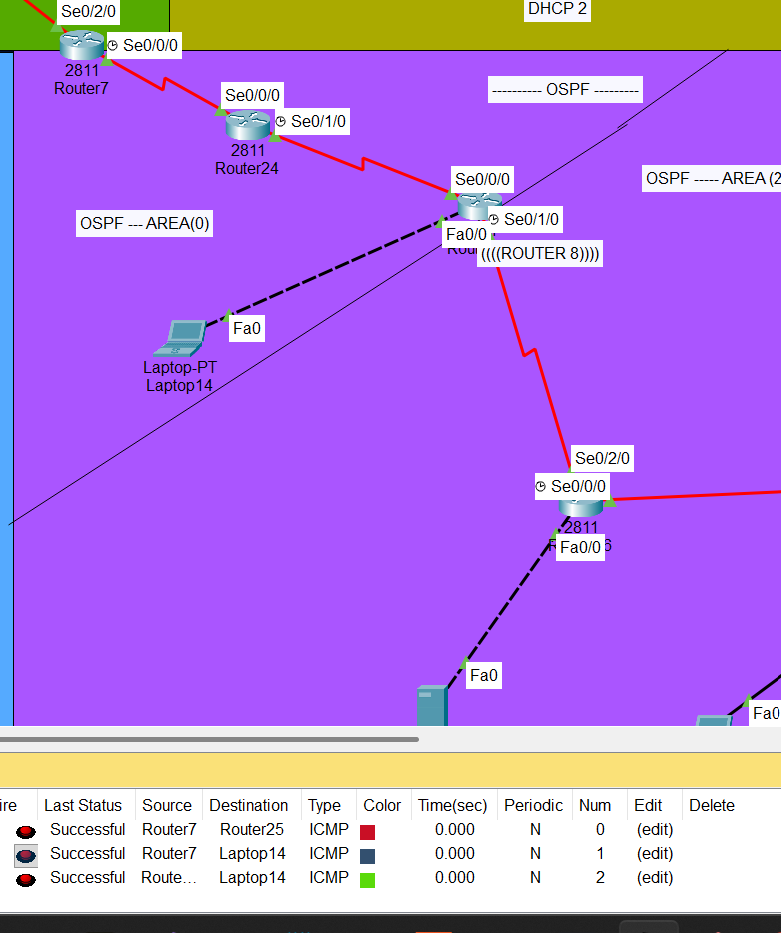
\includegraphics[width=0.6\textwidth]{results/ospf_area0_message.png}
    \caption{OSPF Area 0 Configuration and Verification}
    \label{fig:ospf-area0}
\end{figure}

\subsection{OSPF Area 1 Configuration}

Figure~\ref{fig:ospf-area1} shows the Area 1 configuration and verification.

\begin{figure}[H]
    \centering
    \begin{subfigure}{0.48\textwidth}
        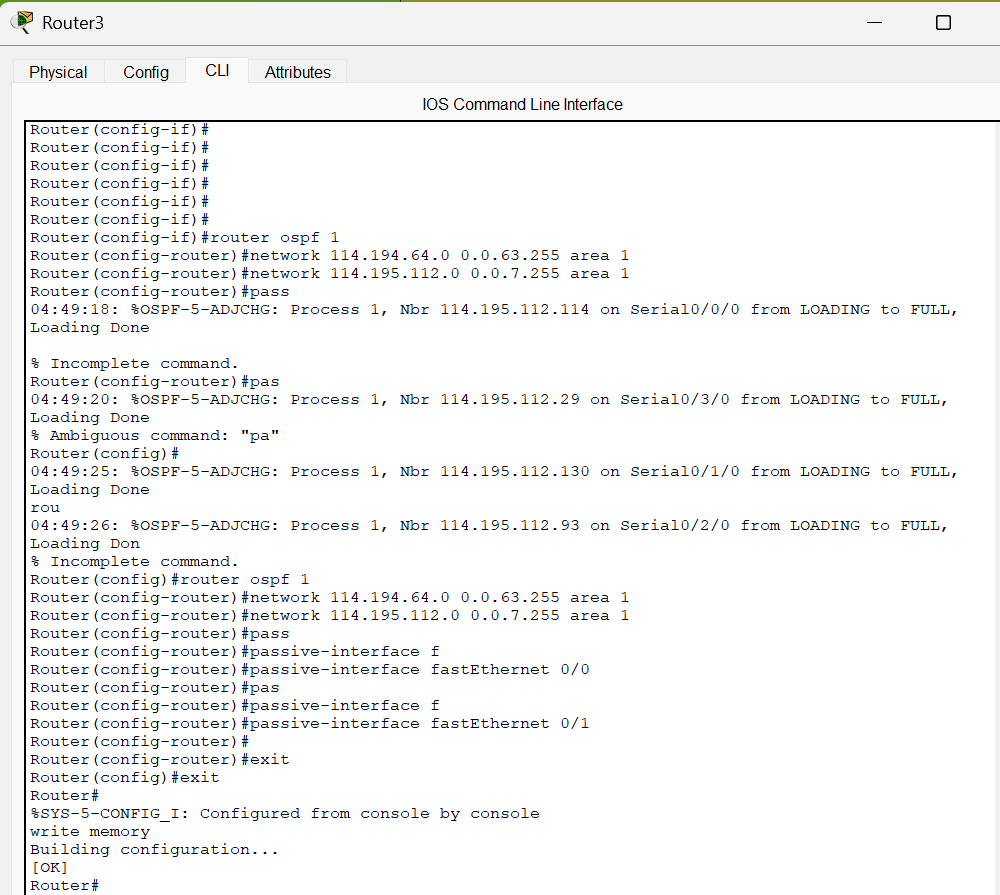
\includegraphics[width=\textwidth]{results/ospf_area1_commands.png}
        \caption{OSPF Area 1 Commands}
    \end{subfigure}
    \hfill
    \begin{subfigure}{0.48\textwidth}
        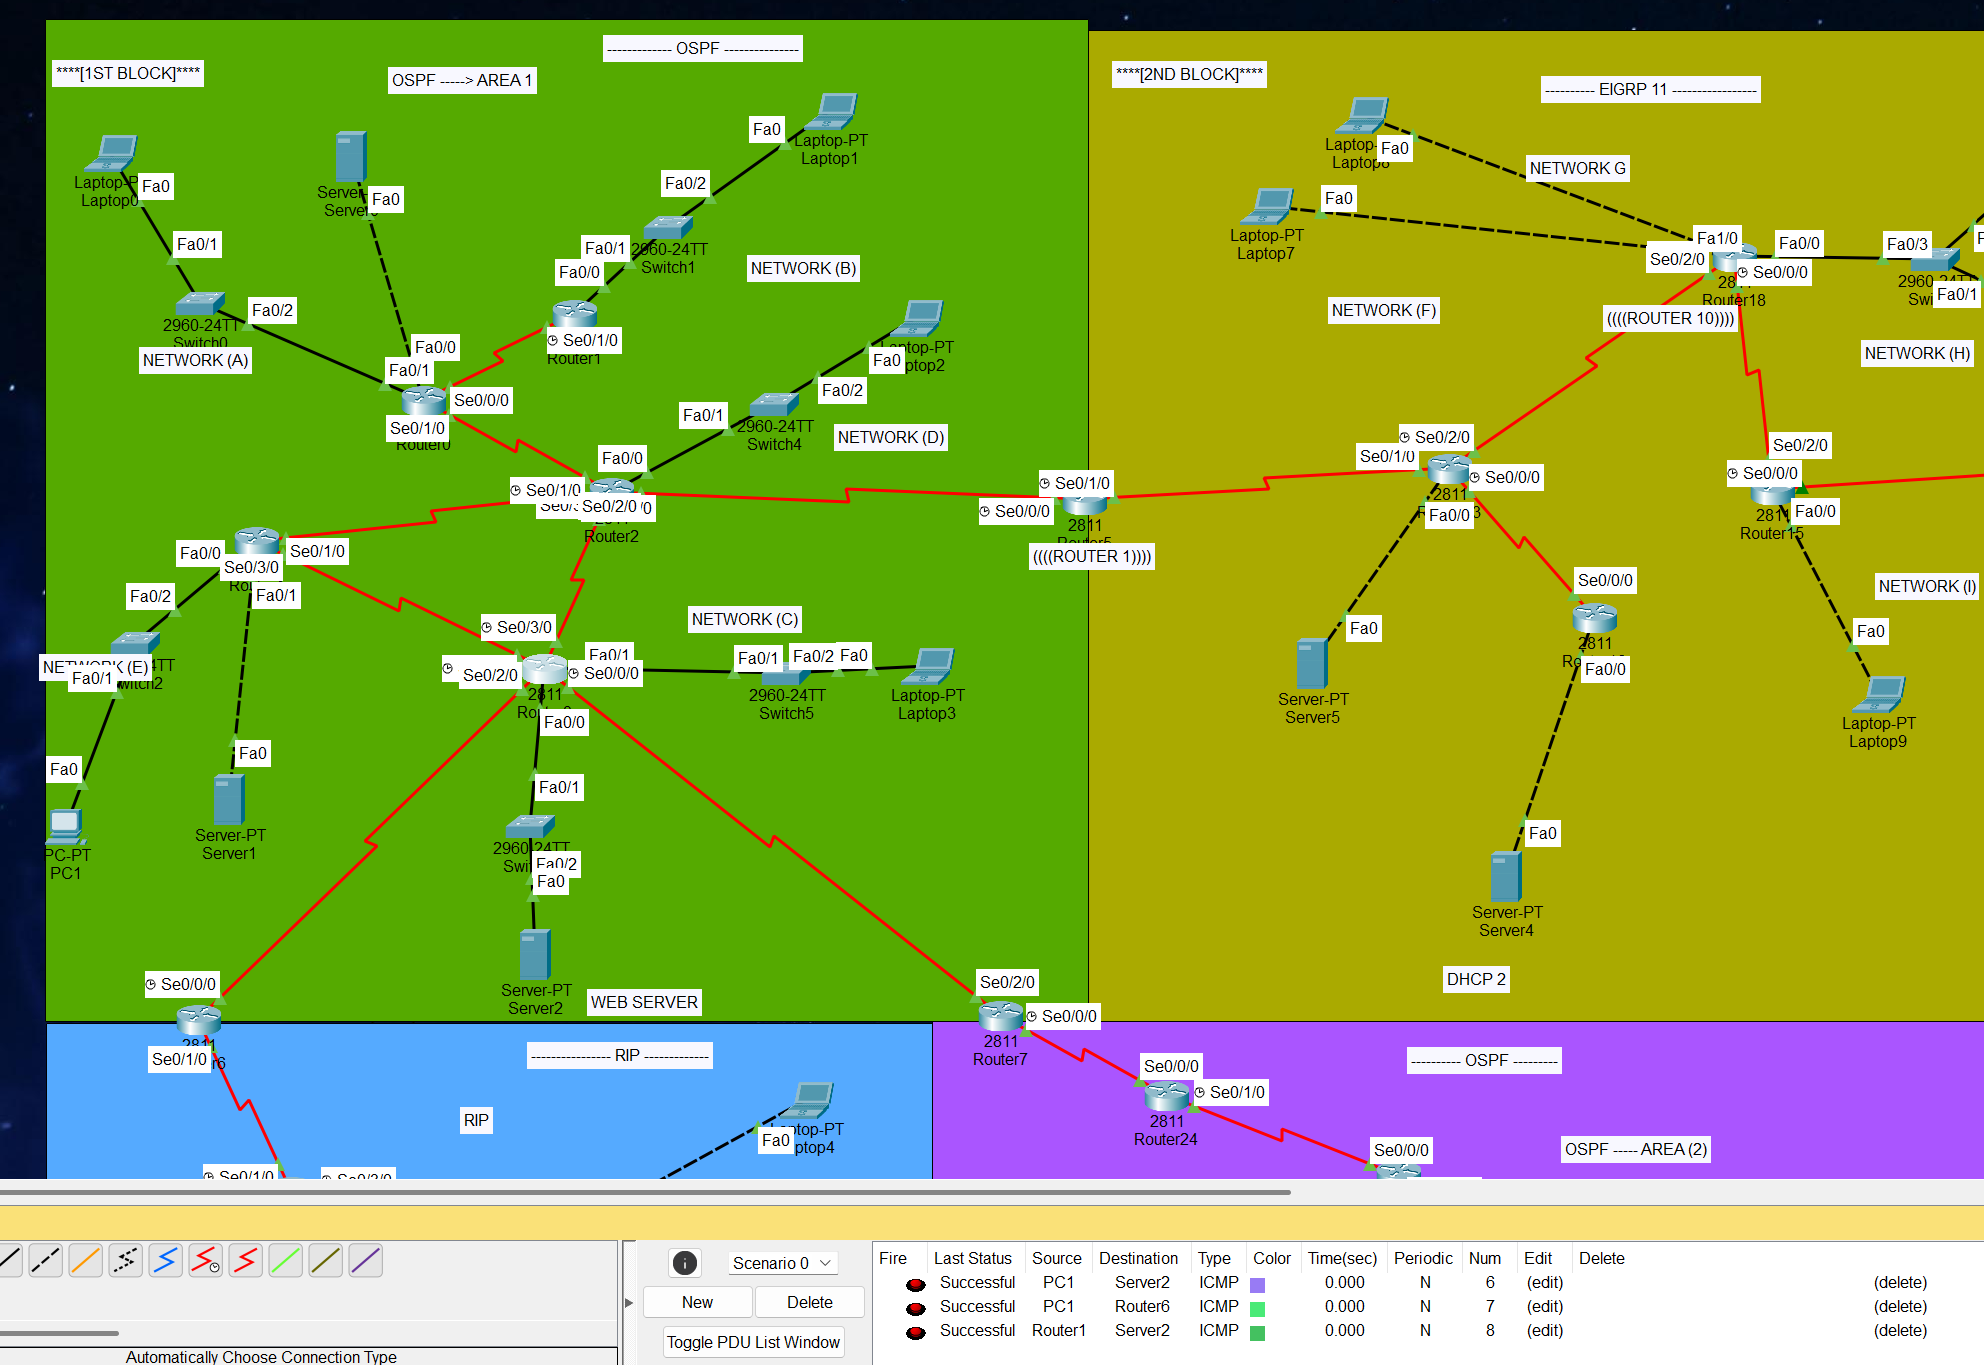
\includegraphics[width=\textwidth]{results/ospf_area1_message.png}
        \caption{OSPF Area 1 Message}
    \end{subfigure}
    \caption{OSPF Area 1 Configuration and Verification}
    \label{fig:ospf-area1}
\end{figure}

\section{EIGRP Configuration}

EIGRP is a hybrid routing protocol that combines features of distance-vector and link-state protocols. Figure~\ref{fig:eigrp-commands} shows the EIGRP configuration.

\begin{figure}[H]
    \centering
    \begin{subfigure}{0.32\textwidth}
        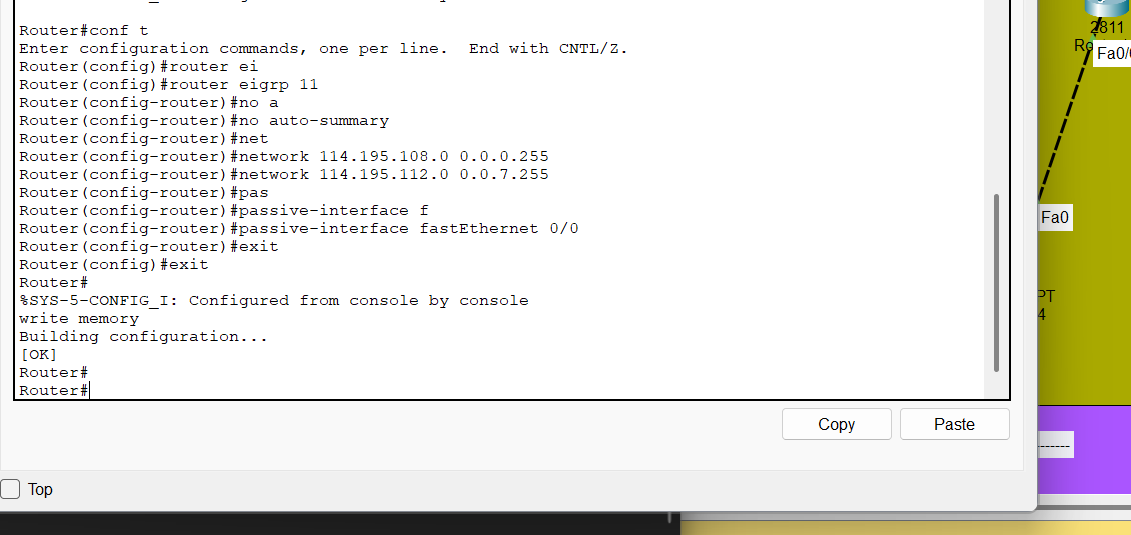
\includegraphics[width=\textwidth]{results/eigrp11_commands.png}
        \caption{EIGRP Commands - Part 1}
    \end{subfigure}
    \hfill
    \begin{subfigure}{0.32\textwidth}
        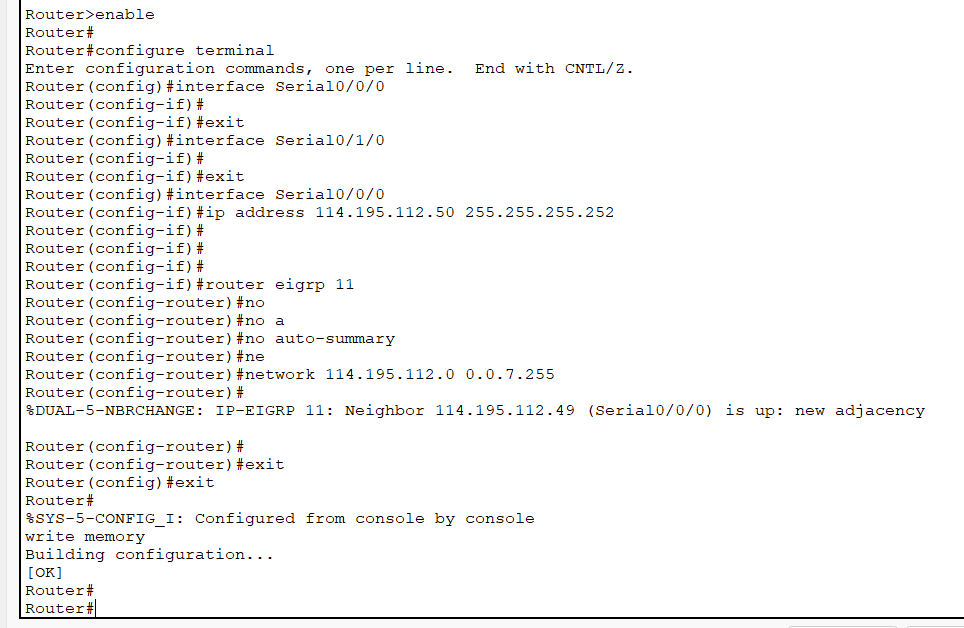
\includegraphics[width=\textwidth]{results/eigrp11_commands_2.png}
        \caption{EIGRP Commands - Part 2}
    \end{subfigure}
    \hfill
    \begin{subfigure}{0.32\textwidth}
        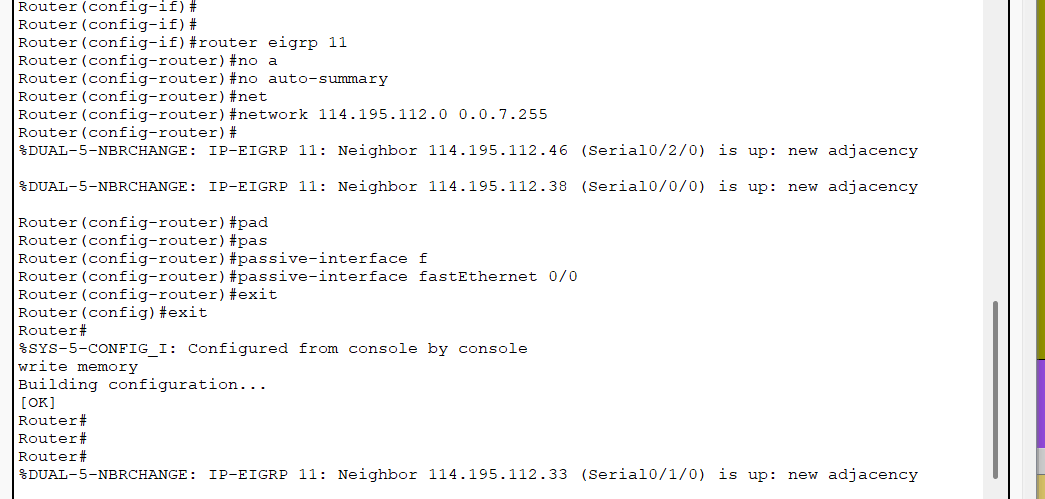
\includegraphics[width=\textwidth]{results/eigrp11_commands_3.png}
        \caption{EIGRP Commands - Part 3}
    \end{subfigure}
    \caption{EIGRP Configuration Commands}
    \label{fig:eigrp-commands}
\end{figure}

\section{Protocol Redistribution}

To enable communication between different routing domains, route redistribution is configured between the protocols.

\subsection{RIP-EIGRP Redistribution}

Figure~\ref{fig:rip-eigrp} shows the RIP-EIGRP redistribution configuration and verification.

\begin{figure}[H]
    \centering
    \begin{subfigure}{0.48\textwidth}
        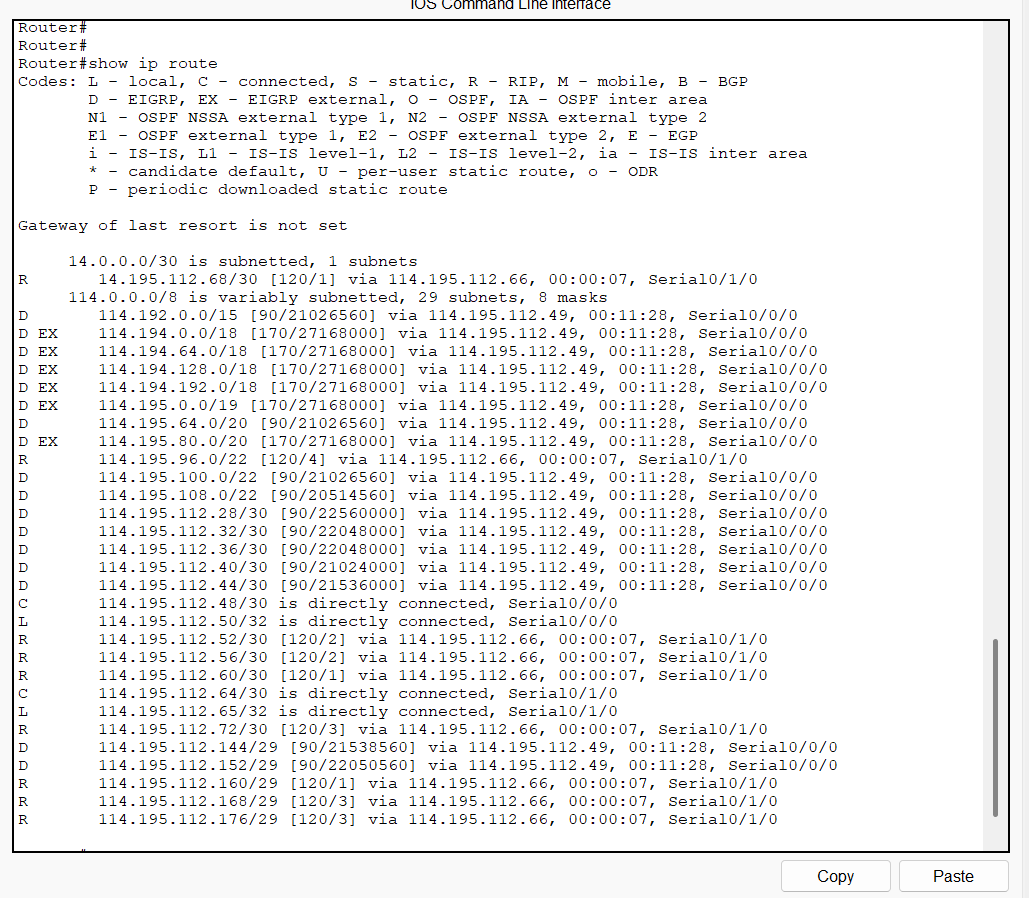
\includegraphics[width=\textwidth]{results/rip-eigrp-proof.png}
        \caption{RIP-EIGRP Redistribution Proof - Part 1}
    \end{subfigure}
    \hfill
    \begin{subfigure}{0.48\textwidth}
        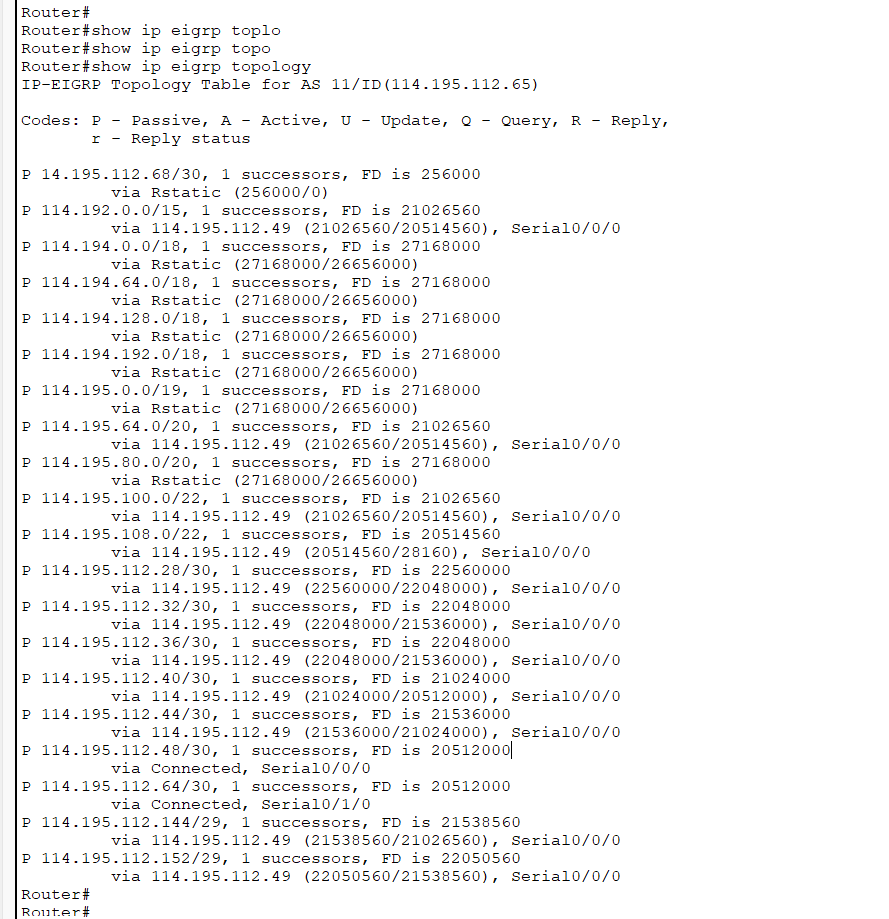
\includegraphics[width=\textwidth]{results/rip-eigrp-proof2.png}
        \caption{RIP-EIGRP Redistribution Proof - Part 2}
    \end{subfigure}
    \vspace{0.5cm}
    \centering
    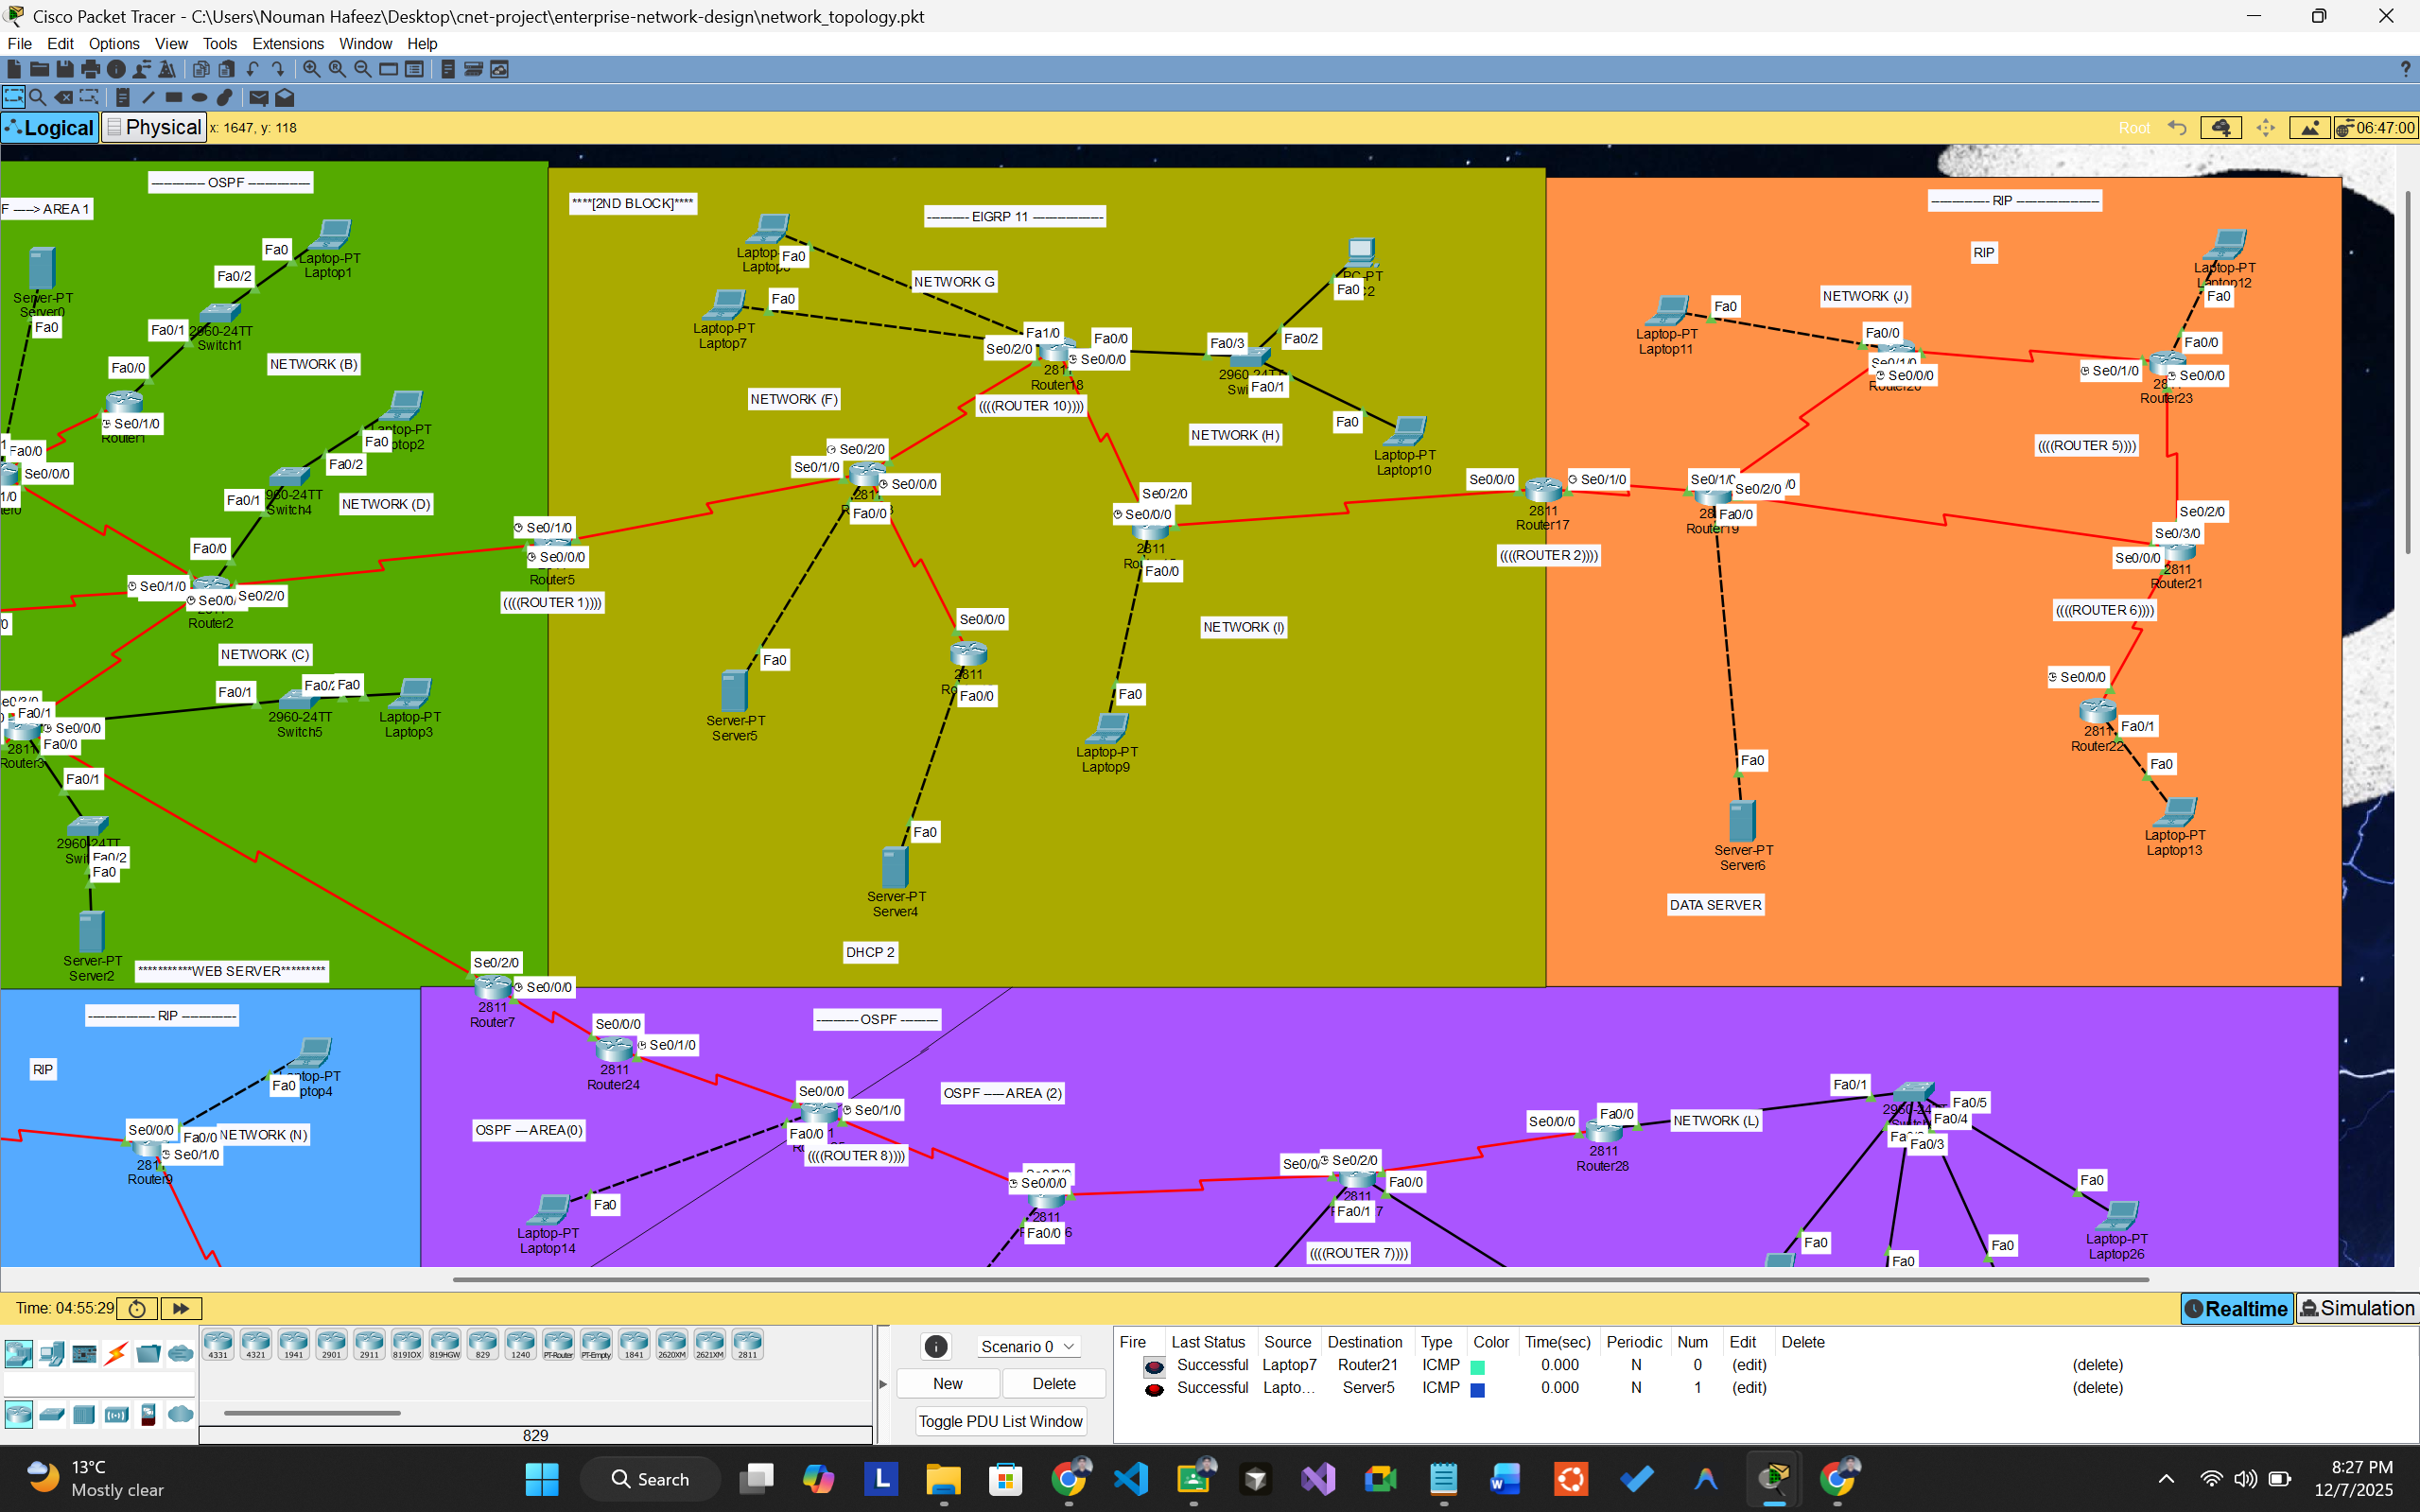
\includegraphics[width=0.6\textwidth]{results/eigrp-rip-redistribution.png}
    \caption{RIP-EIGRP Redistribution Configuration and Verification}
    \label{fig:rip-eigrp}
\end{figure}

\subsection{OSPF Redistribution}

\subsubsection{OSPF Area 1 Redistribution}

Figure~\ref{fig:ospf-redist-1} shows OSPF Area 1 redistribution with RIP and EIGRP.

\begin{figure}[H]
    \centering
    \begin{subfigure}{0.48\textwidth}
        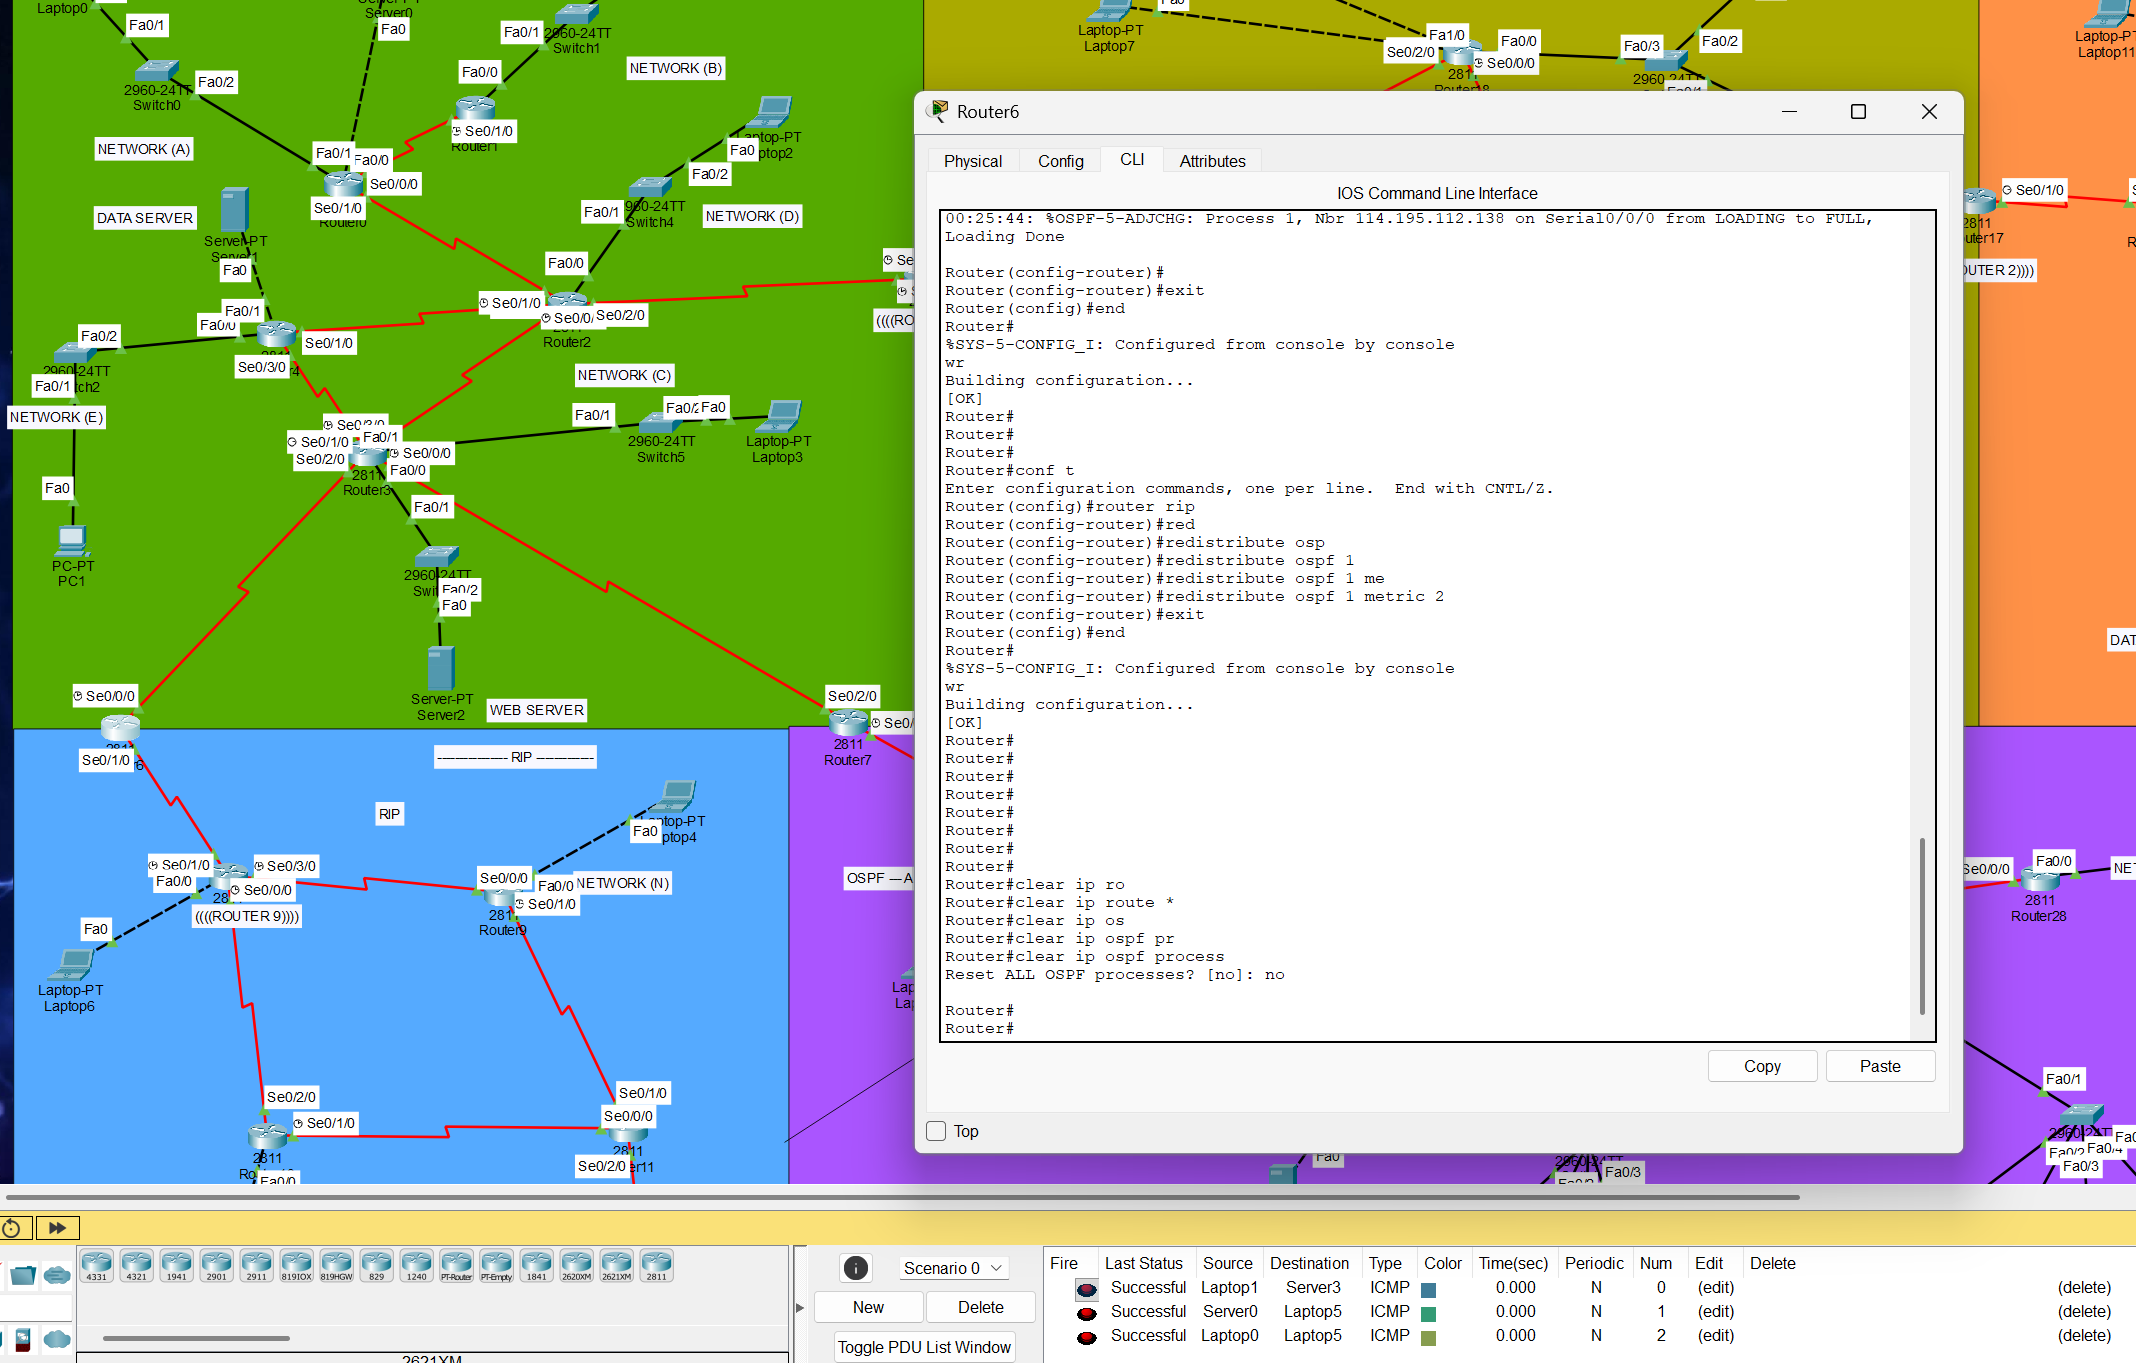
\includegraphics[width=\textwidth]{results/area1(ospf)_rip_redistribution.png}
        \caption{OSPF Area 1 - RIP Redistribution}
    \end{subfigure}
    \hfill
    \begin{subfigure}{0.48\textwidth}
        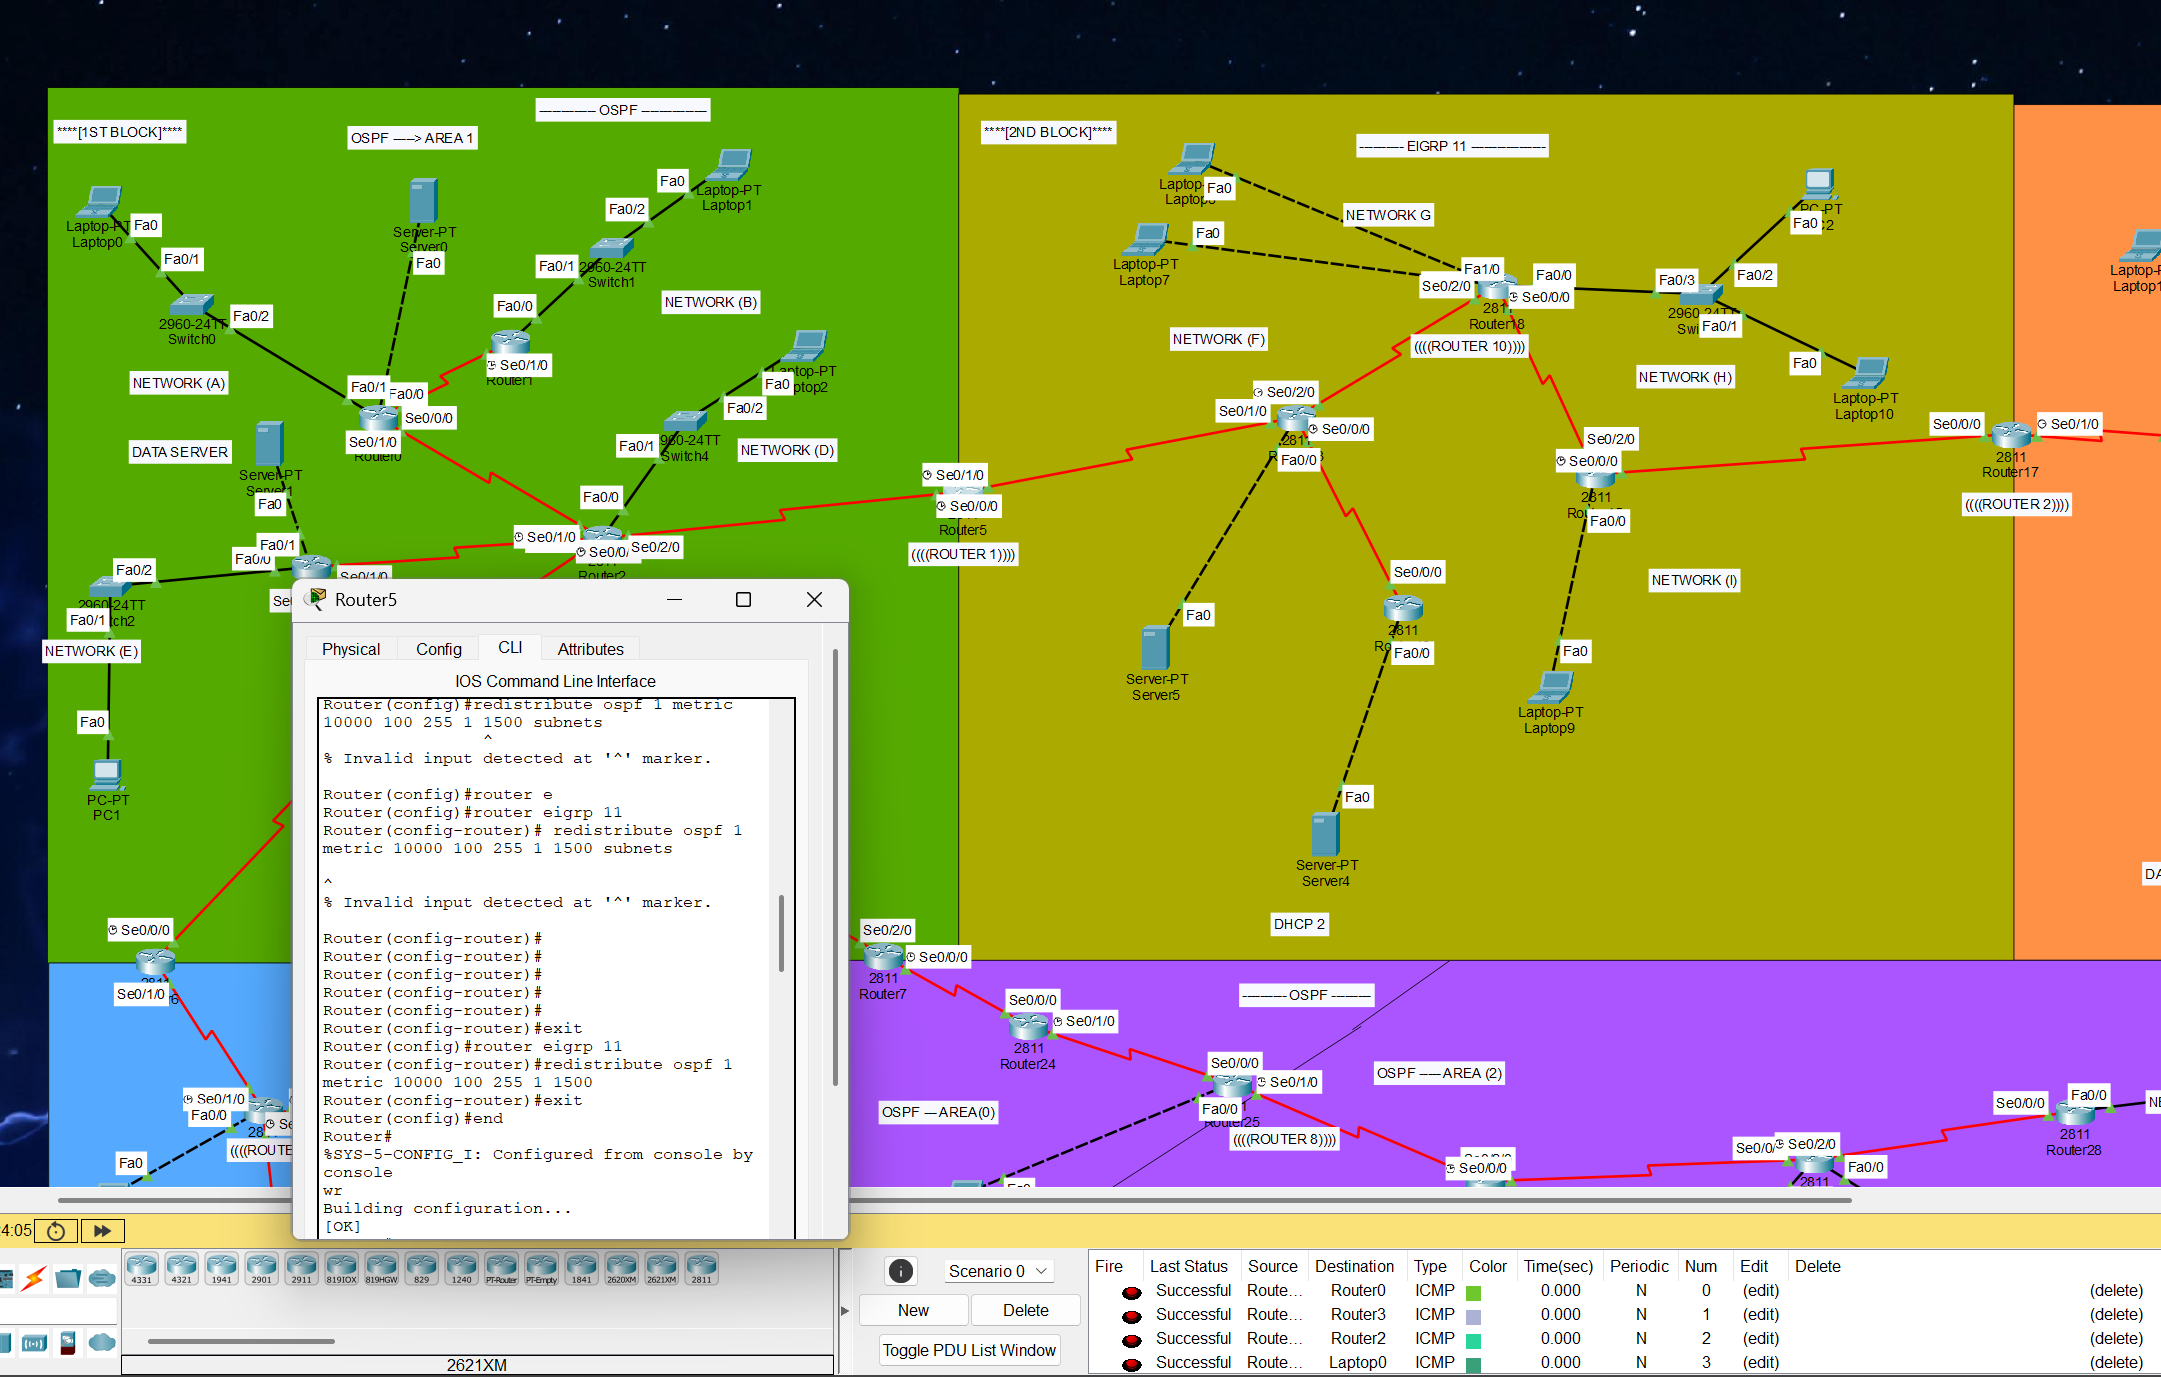
\includegraphics[width=\textwidth]{results/area1(ospf)_eigrp_redistribution.png}
        \caption{OSPF Area 1 - EIGRP Redistribution}
    \end{subfigure}
    \caption{OSPF Area 1 Redistribution}
    \label{fig:ospf-redist-1}
\end{figure}

\subsubsection{OSPF Inter-Area Redistribution}

Figure~\ref{fig:ospf-inter-area} shows OSPF inter-area redistribution between Area 0, Area 1, and Area 2.

\begin{figure}[H]
    \centering
    \begin{subfigure}{0.48\textwidth}
        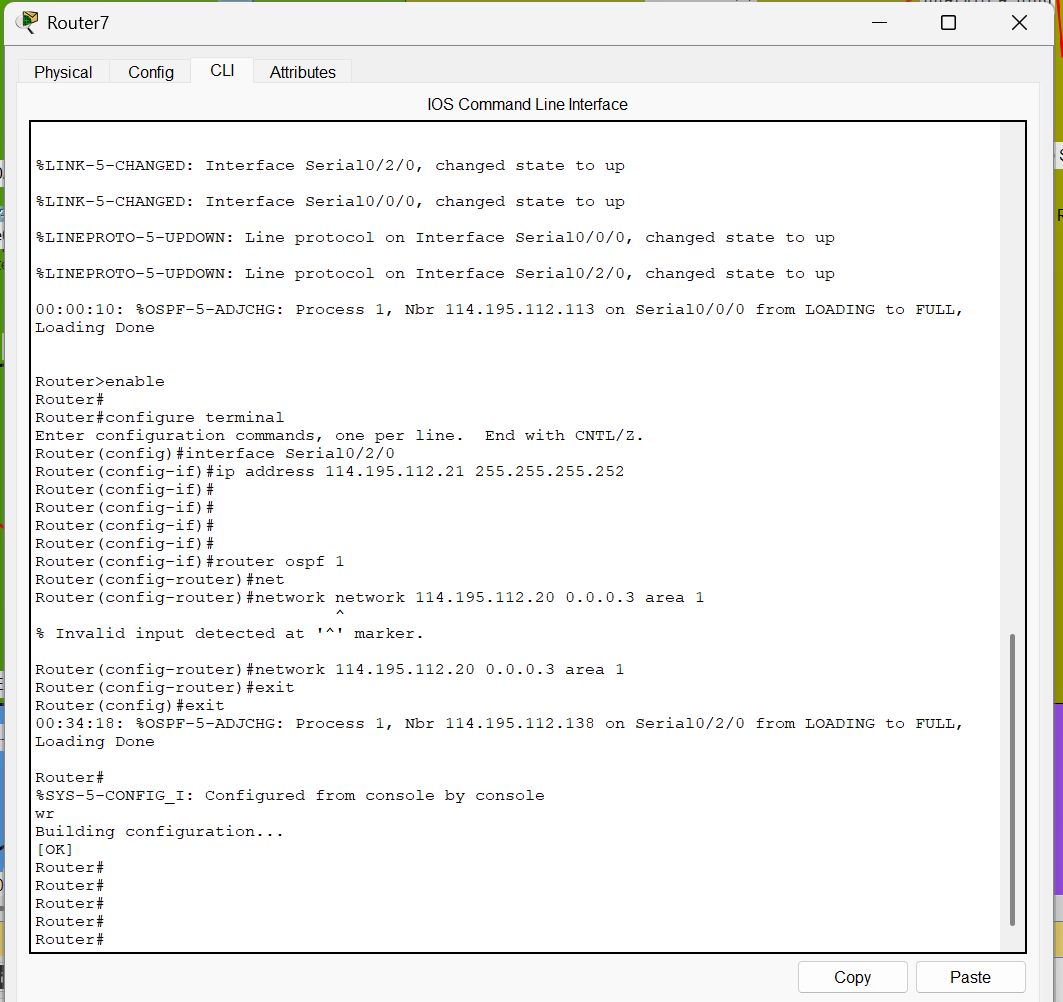
\includegraphics[width=\textwidth]{results/area1_area0_ospf_redistribution.png}
        \caption{OSPF Area 1 - Area 0 Redistribution}
    \end{subfigure}
    \hfill
    \begin{subfigure}{0.48\textwidth}
        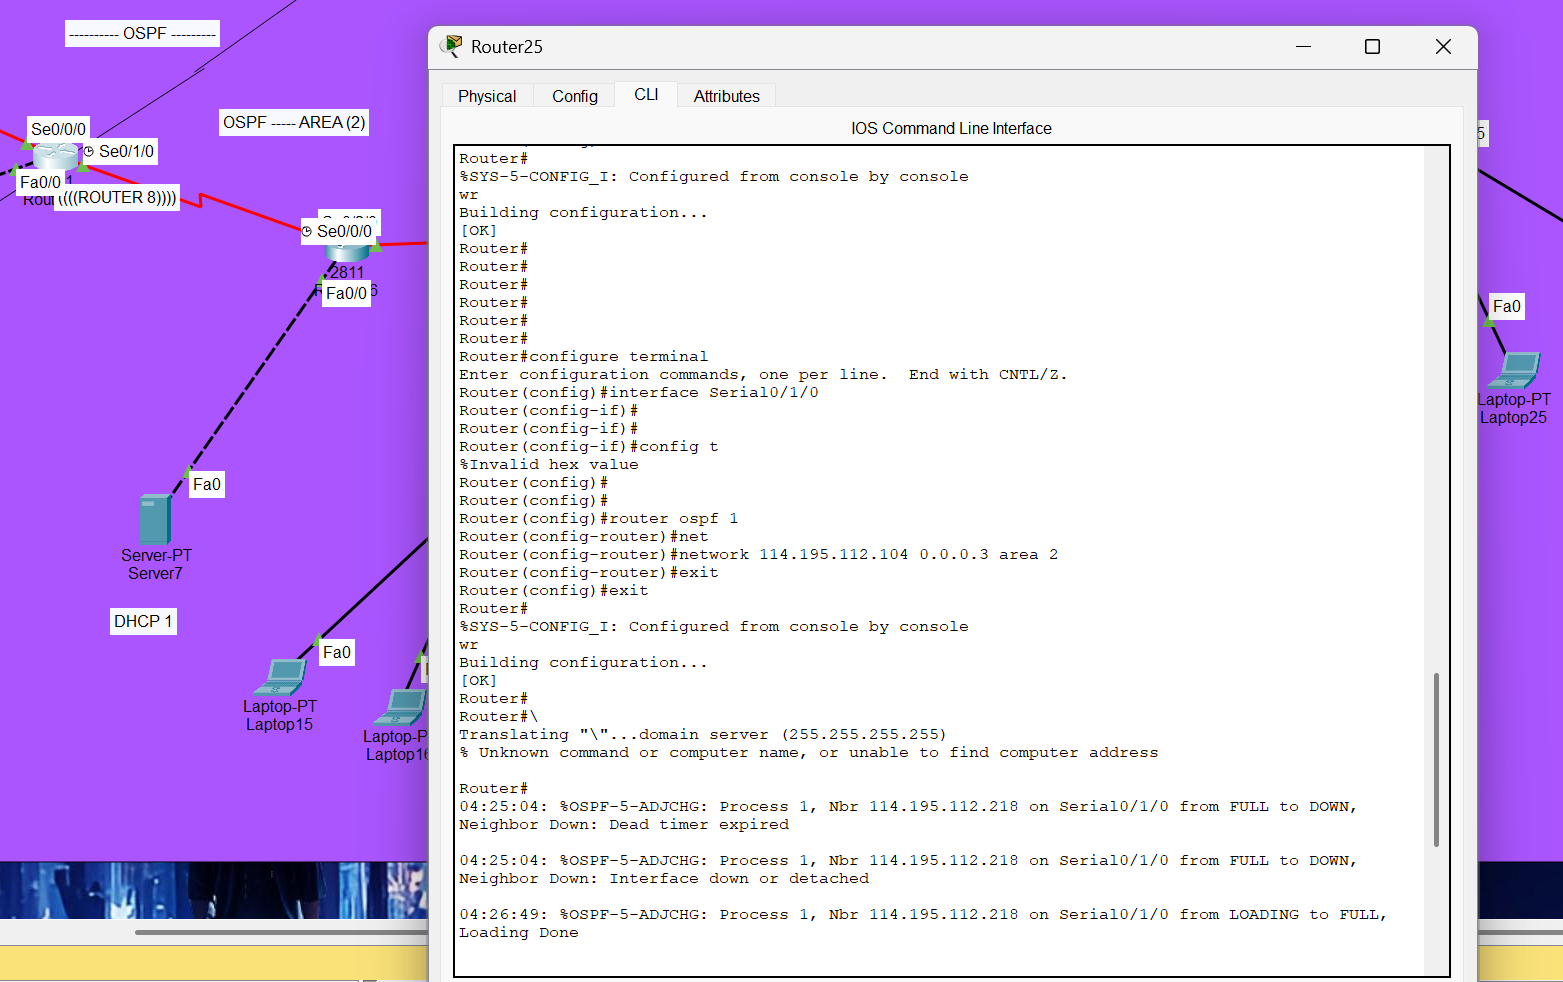
\includegraphics[width=\textwidth]{results/area0_area2_ospf_redistribution.png}
        \caption{OSPF Area 0 - Area 2 Redistribution}
    \end{subfigure}
    \vspace{0.5cm}
    \centering
    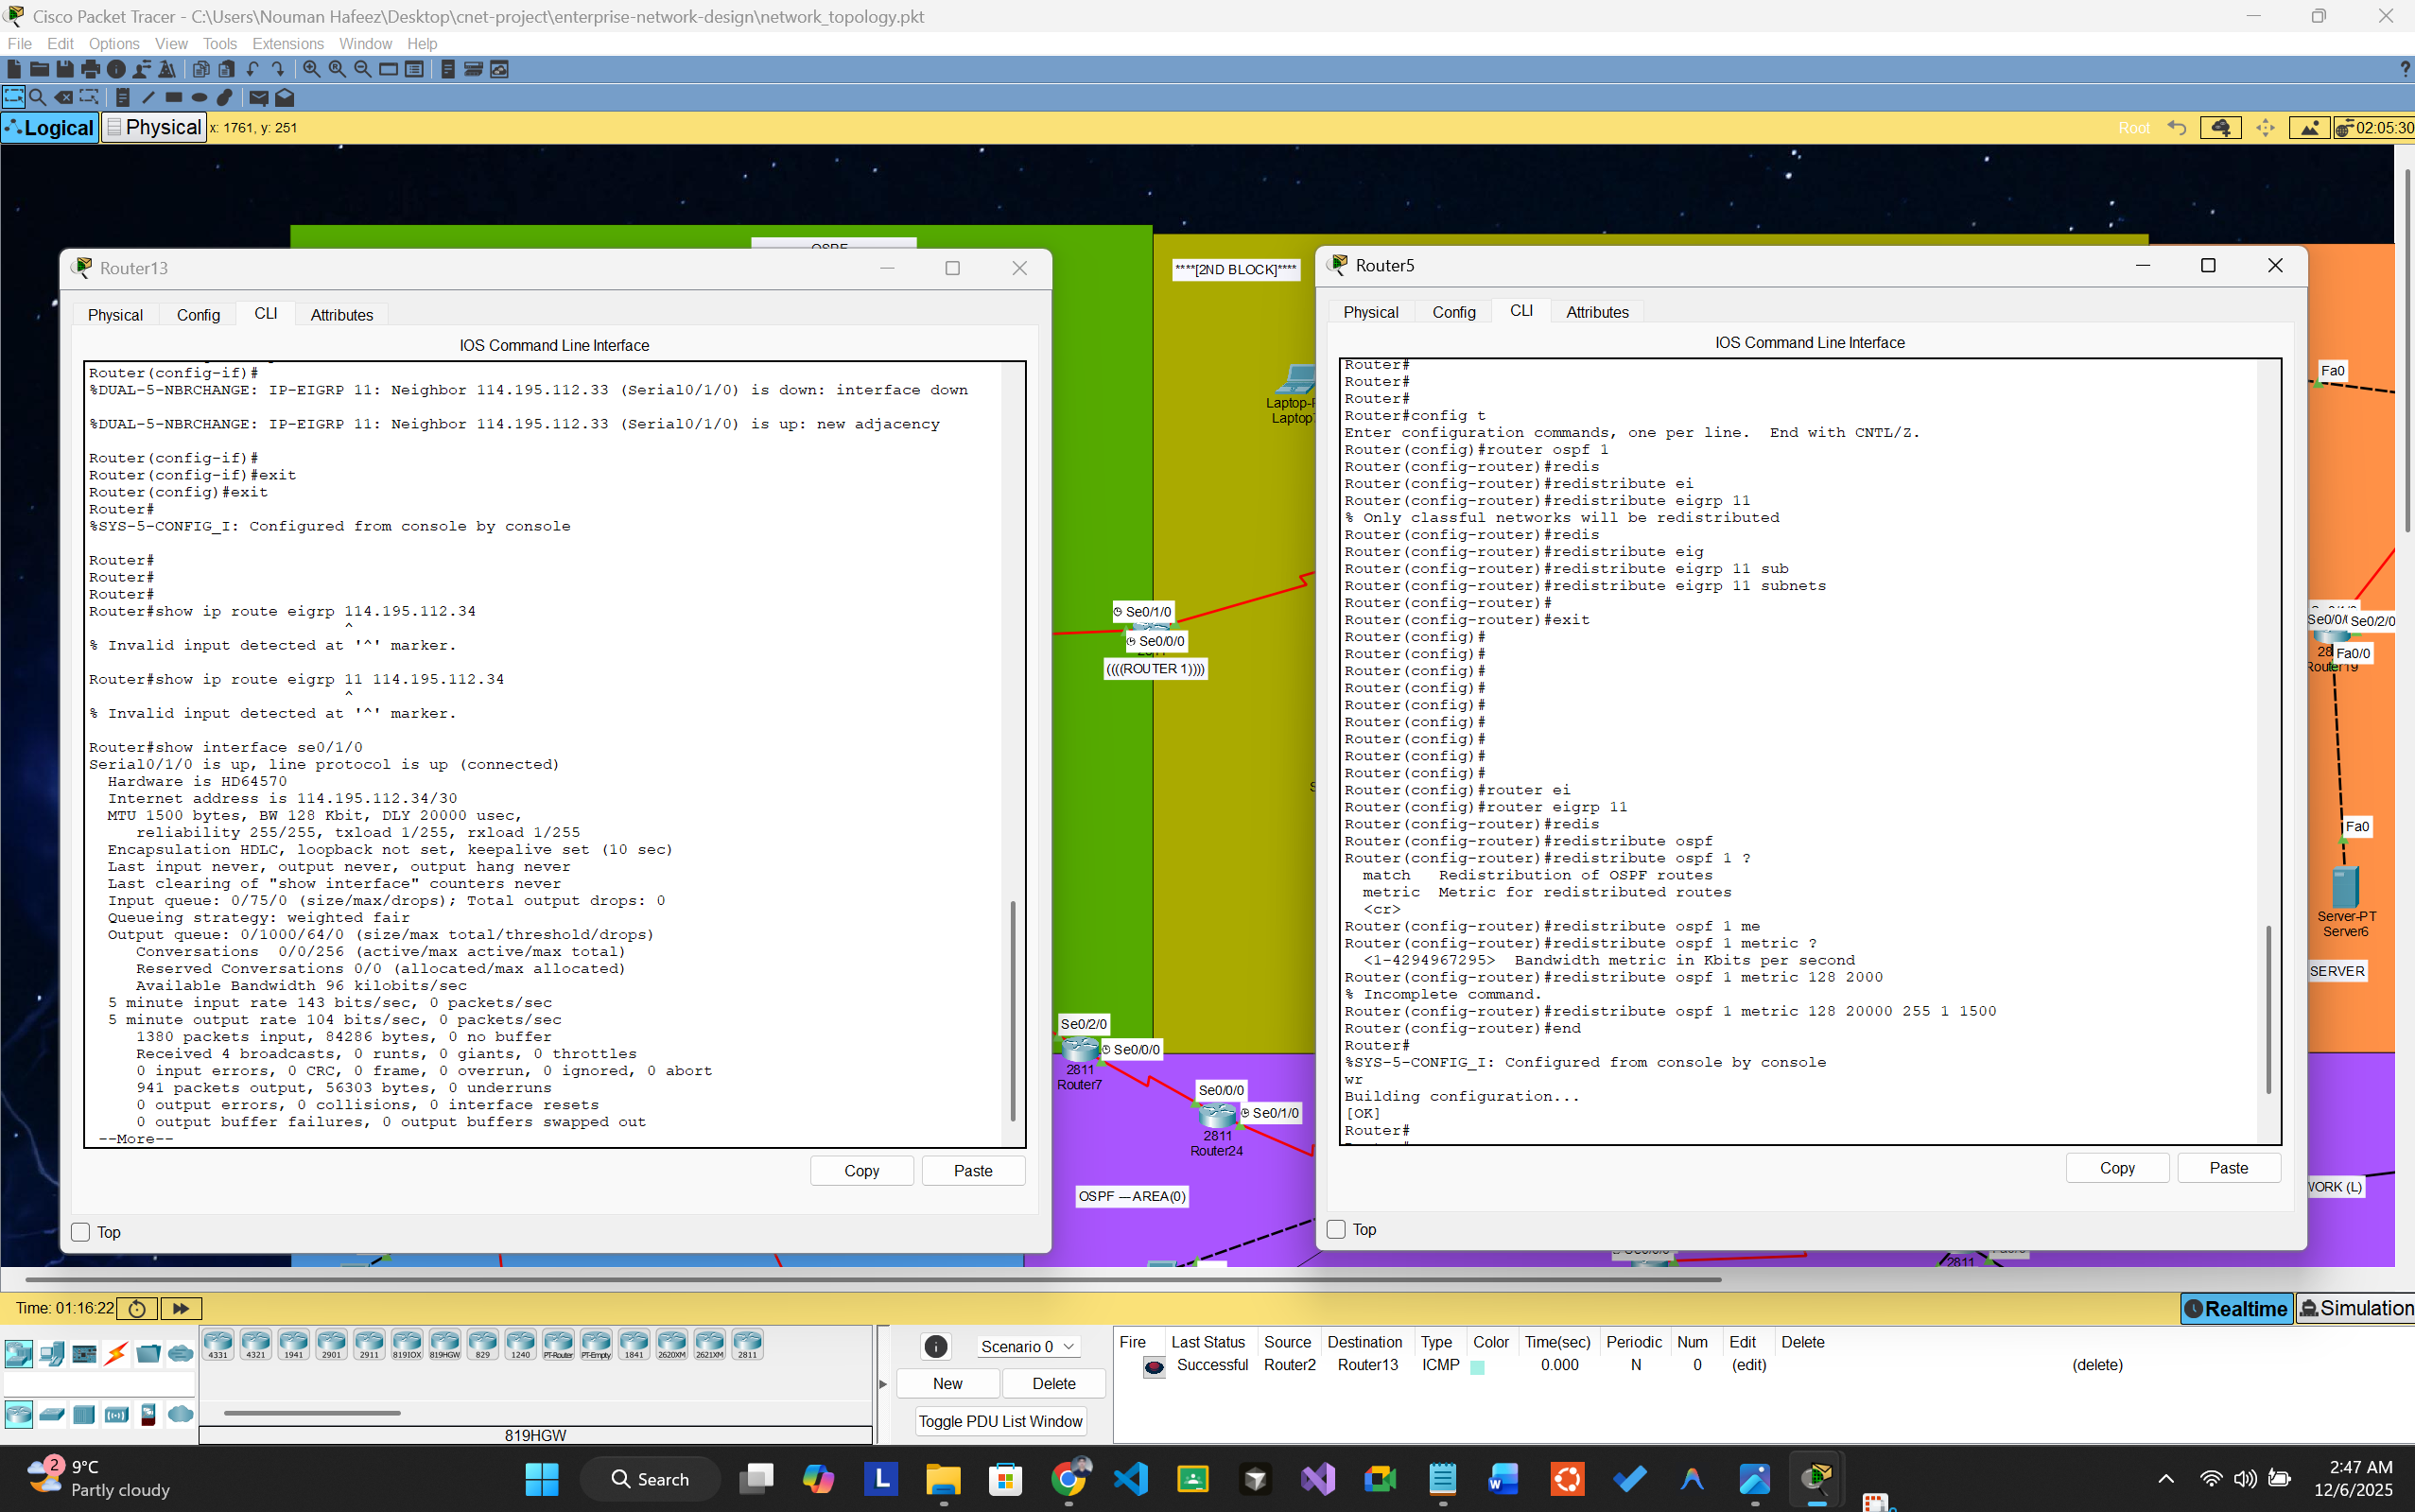
\includegraphics[width=0.6\textwidth]{results/ospf-eigrp11_redistribution.png}
    \caption{OSPF Inter-Area and EIGRP Redistribution}
    \label{fig:ospf-inter-area}
\end{figure}

\newpage

% Chapter 4: DHCP Configuration
\chapter{DHCP Configuration}

Dynamic Host Configuration Protocol (DHCP) is configured to automatically assign IP addresses to network devices. This chapter documents the DHCP server configuration for different network segments.

\section{DHCP Server 1 Configuration}

DHCP Server 1 is configured for Row 2 networks. Figure~\ref{fig:dhcp1} shows the DHCP Server 1 configuration and verification.

\begin{figure}[H]
    \centering
    \begin{subfigure}{0.48\textwidth}
        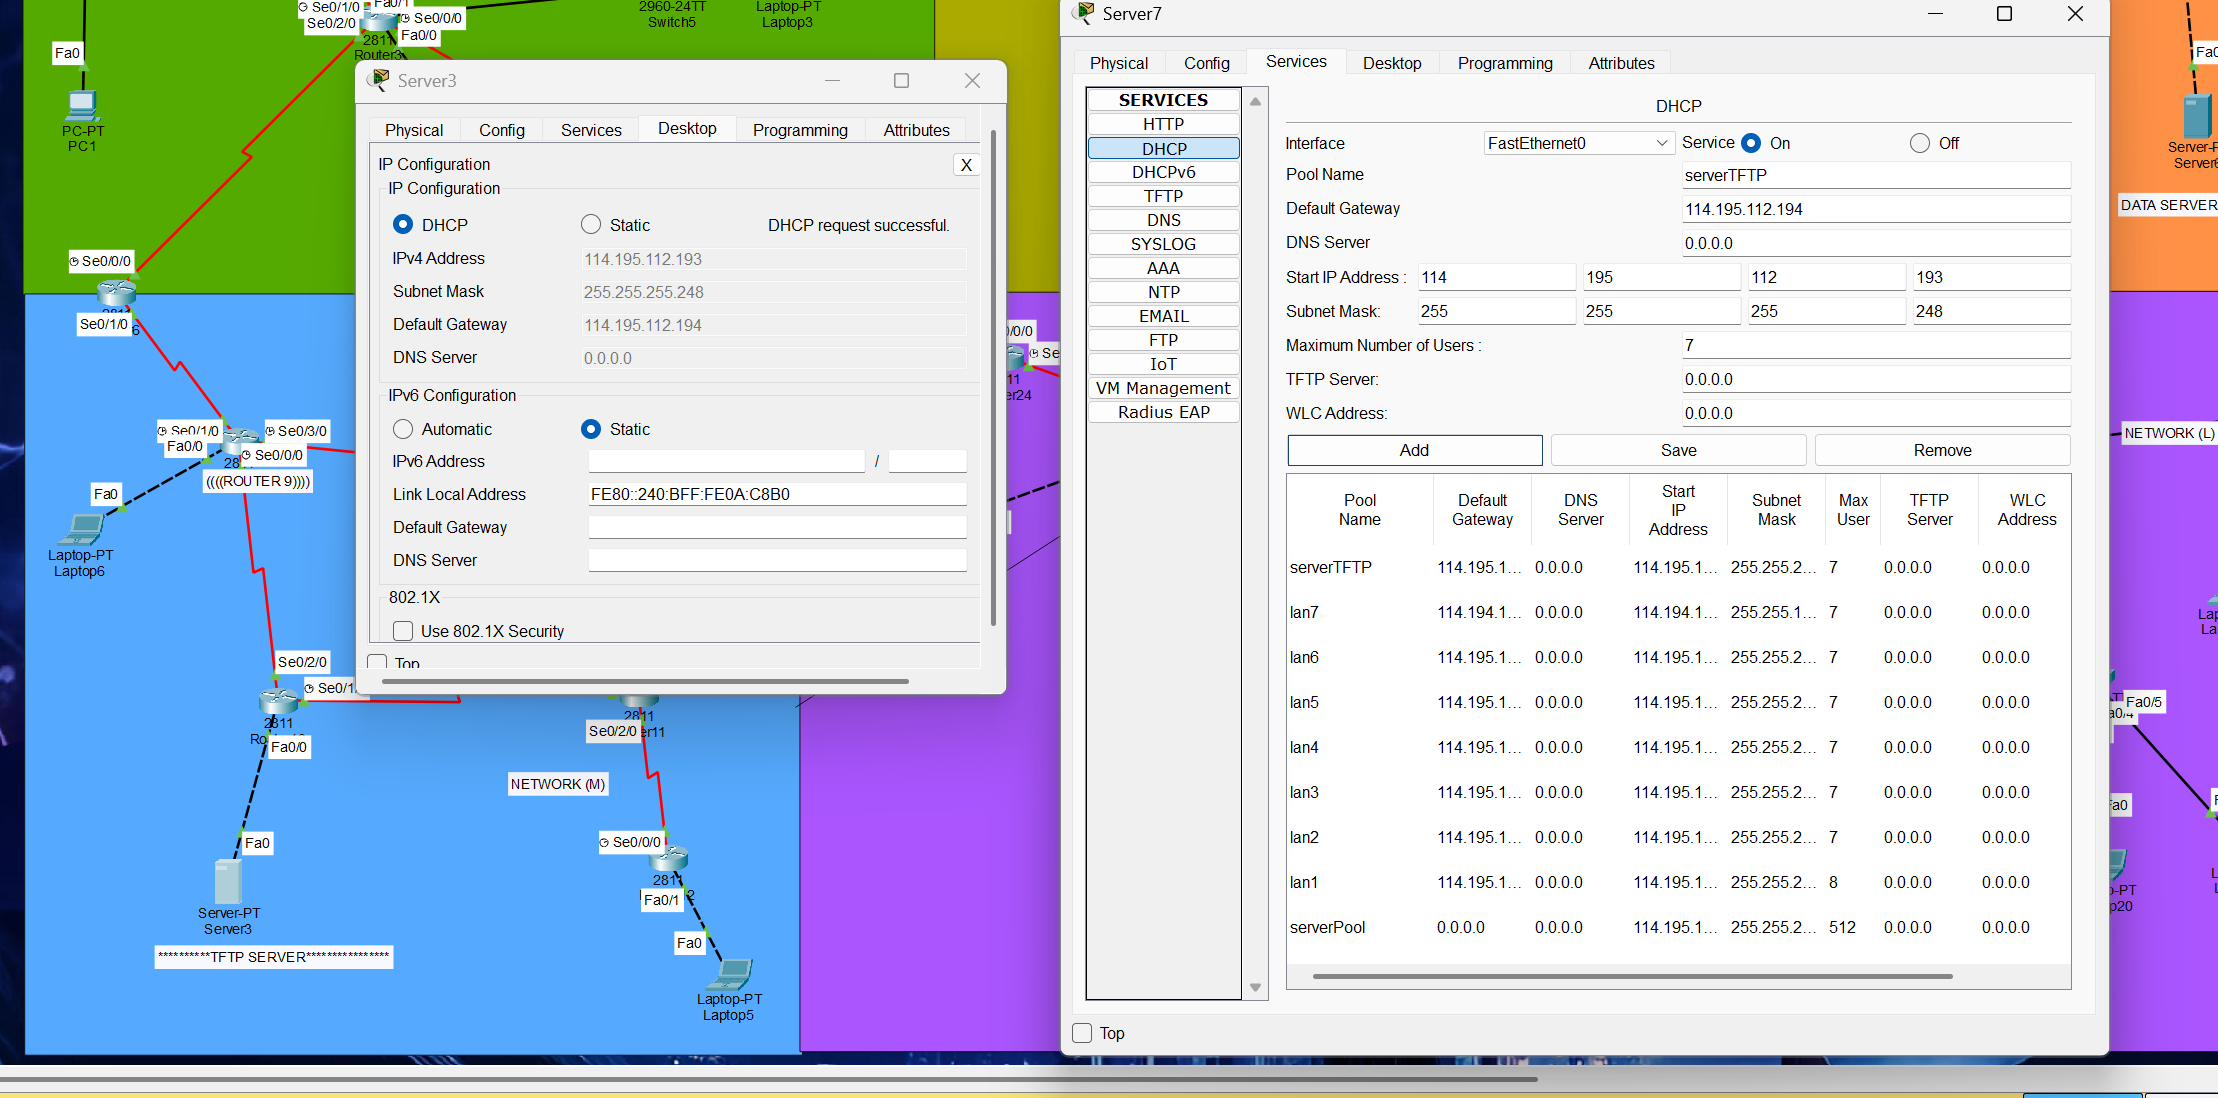
\includegraphics[width=\textwidth]{results/DHCP1-SERVER-TFTP.png}
        \caption{DHCP Server 1 - TFTP Configuration}
    \end{subfigure}
    \hfill
    \begin{subfigure}{0.48\textwidth}
        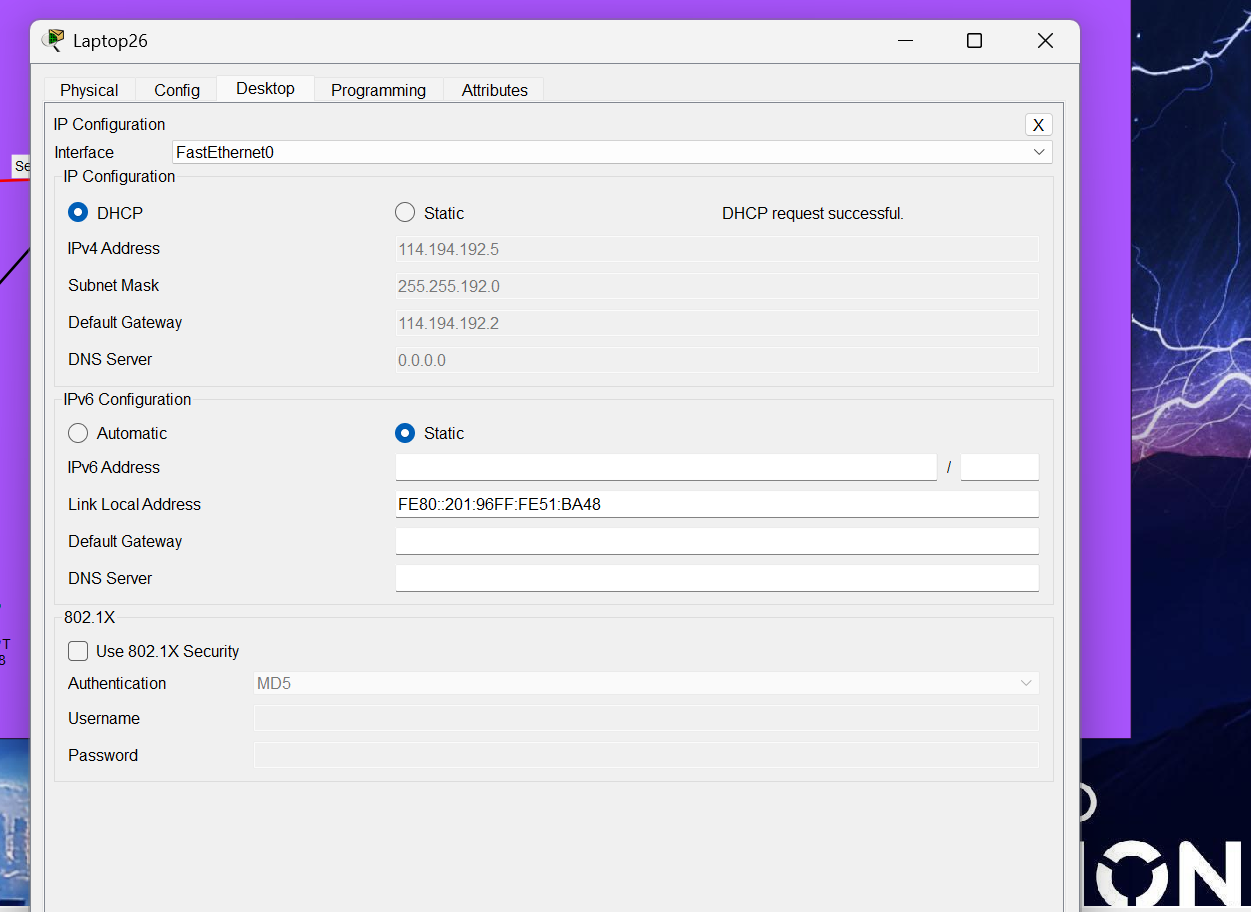
\includegraphics[width=\textwidth]{results/DHCP1-ROW2.png}
        \caption{DHCP Server 1 - Row 2 Configuration}
    \end{subfigure}
    \vspace{0.5cm}
    \centering
    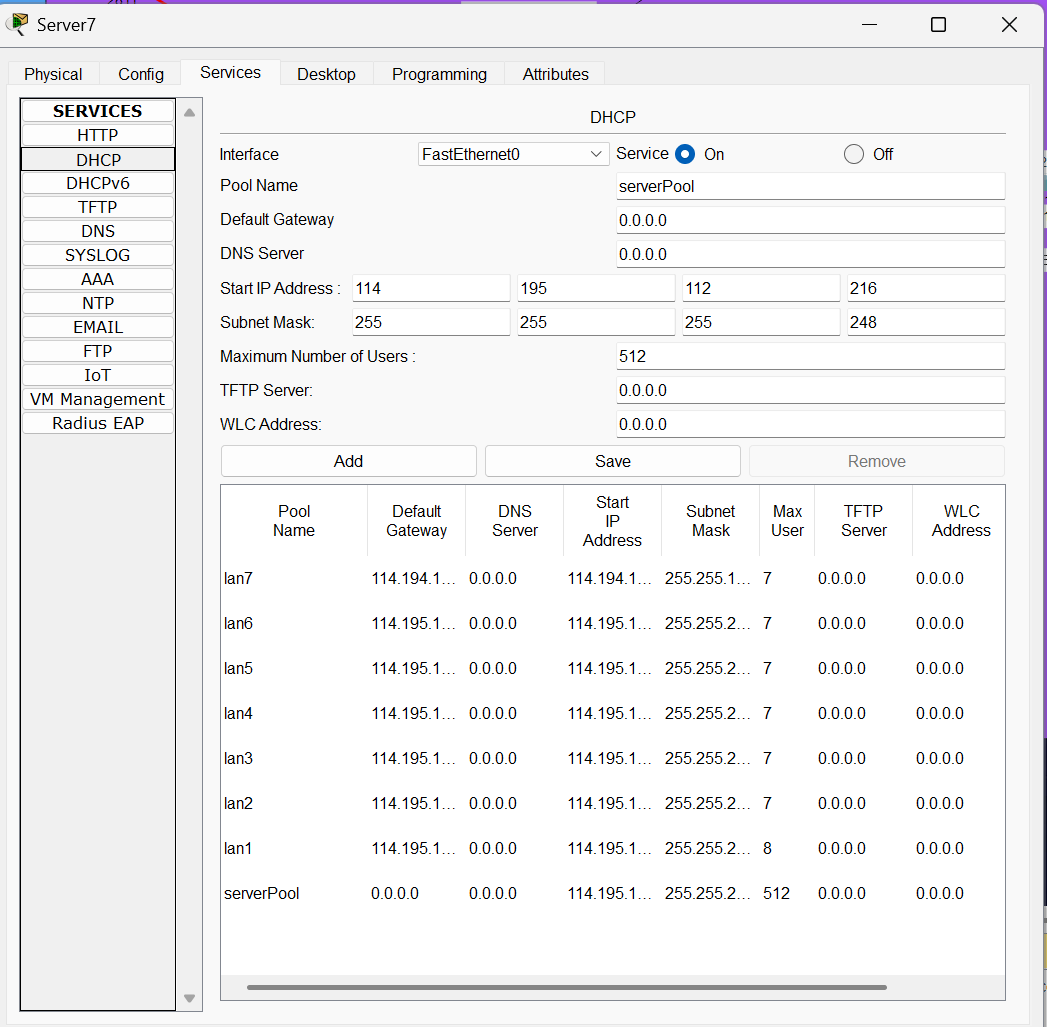
\includegraphics[width=0.6\textwidth]{results/DHCP1-POOLING-ROW2.png}
    \caption{DHCP Server 1 Configuration and Pool Verification}
    \label{fig:dhcp1}
\end{figure}

\section{DHCP Server 2 Configuration}

DHCP Server 2 is configured for Row 1 networks. Figure~\ref{fig:dhcp2} shows the DHCP Server 2 configuration and verification.

\begin{figure}[H]
    \centering
    \begin{subfigure}{0.48\textwidth}
        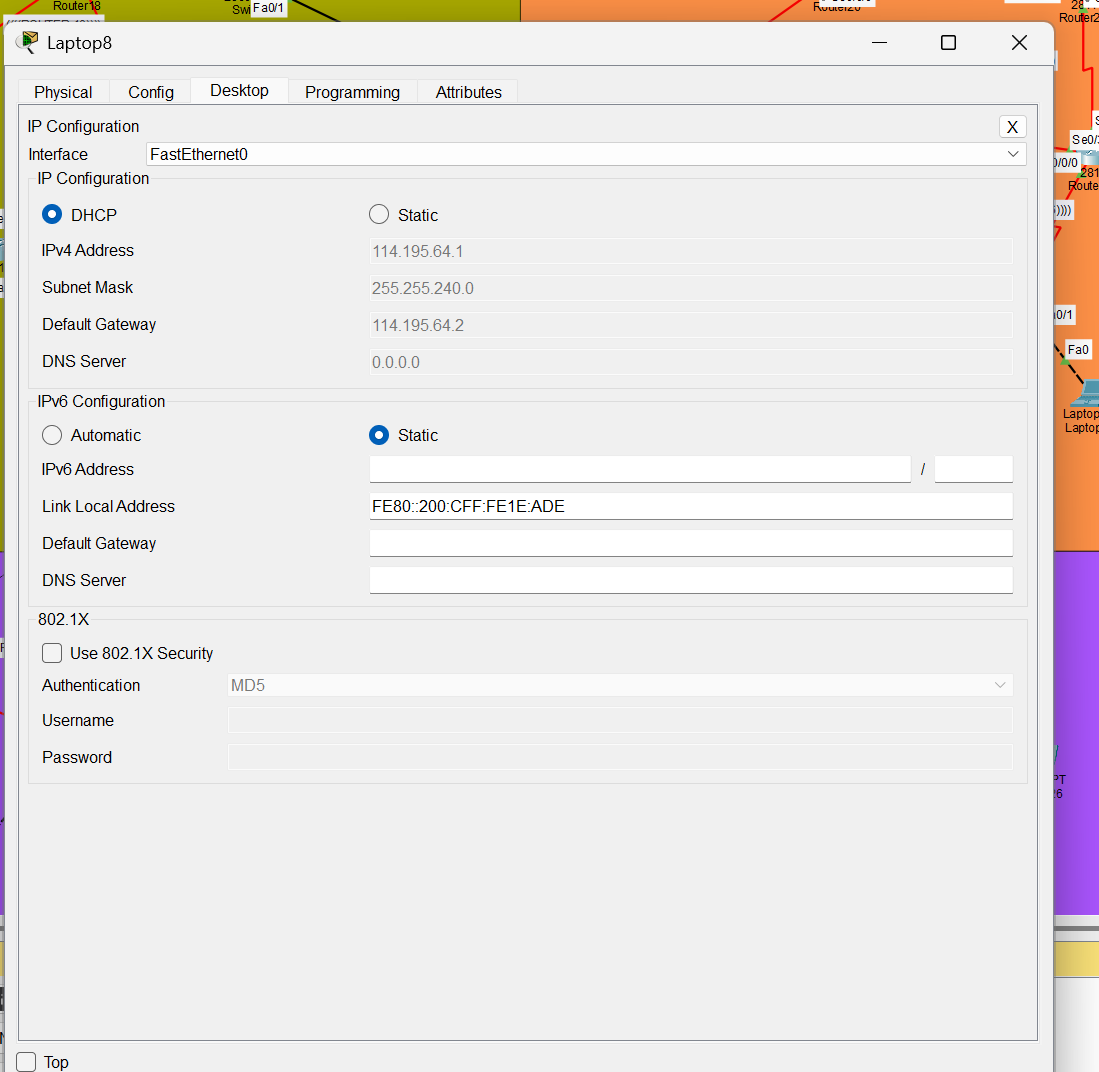
\includegraphics[width=\textwidth]{results/DHCP2-ROW1.png}
        \caption{DHCP Server 2 - Row 1 Configuration}
    \end{subfigure}
    \hfill
    \begin{subfigure}{0.48\textwidth}
        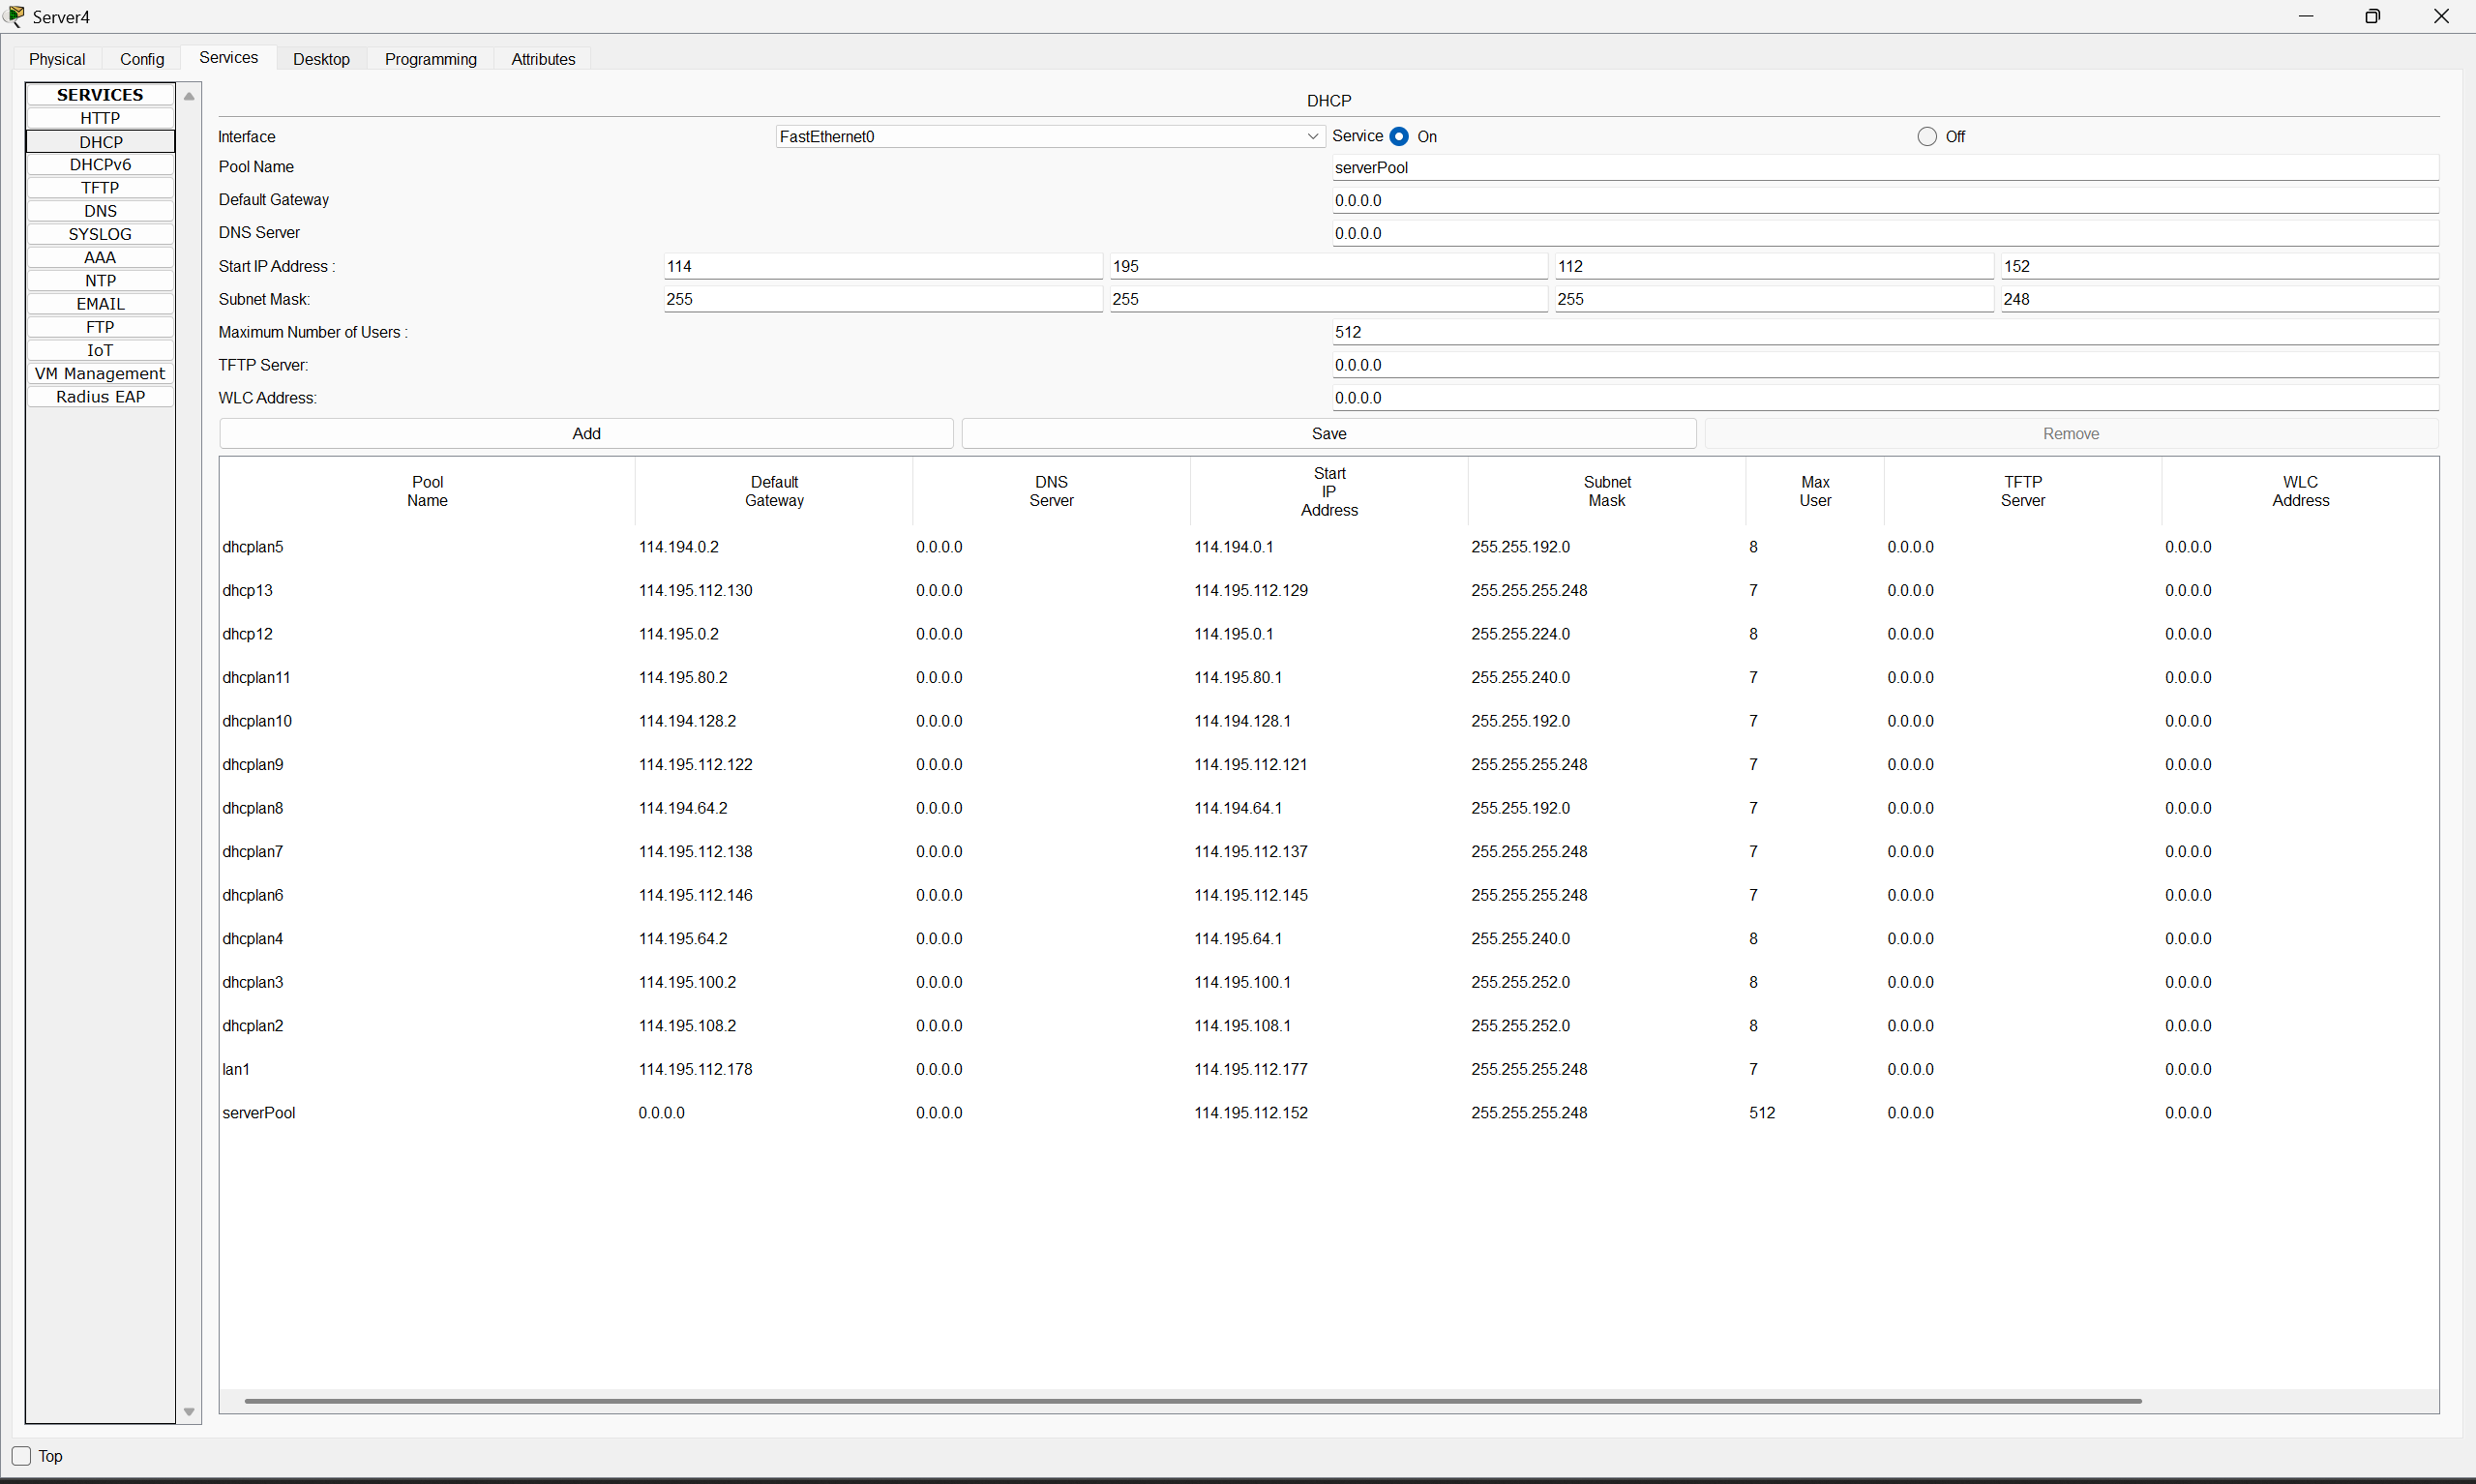
\includegraphics[width=\textwidth]{results/DHCP2-POOLING-ROW1.png}
        \caption{DHCP Server 2 - Pool Verification}
    \end{subfigure}
    \caption{DHCP Server 2 Configuration and Verification}
    \label{fig:dhcp2}
\end{figure}

\newpage

% Chapter 5: Access Control Lists
\chapter{Access Control Lists (ACLs)}

Access Control Lists are configured to control network traffic and enhance security by filtering packets based on source/destination IP addresses and ports.

\section{ACL Configuration for Network 1}

Network 1 (Network L) has ACLs configured for the Web Server. Figure~\ref{fig:acl-network1} shows the ACL configuration.

\begin{figure}[H]
    \centering
    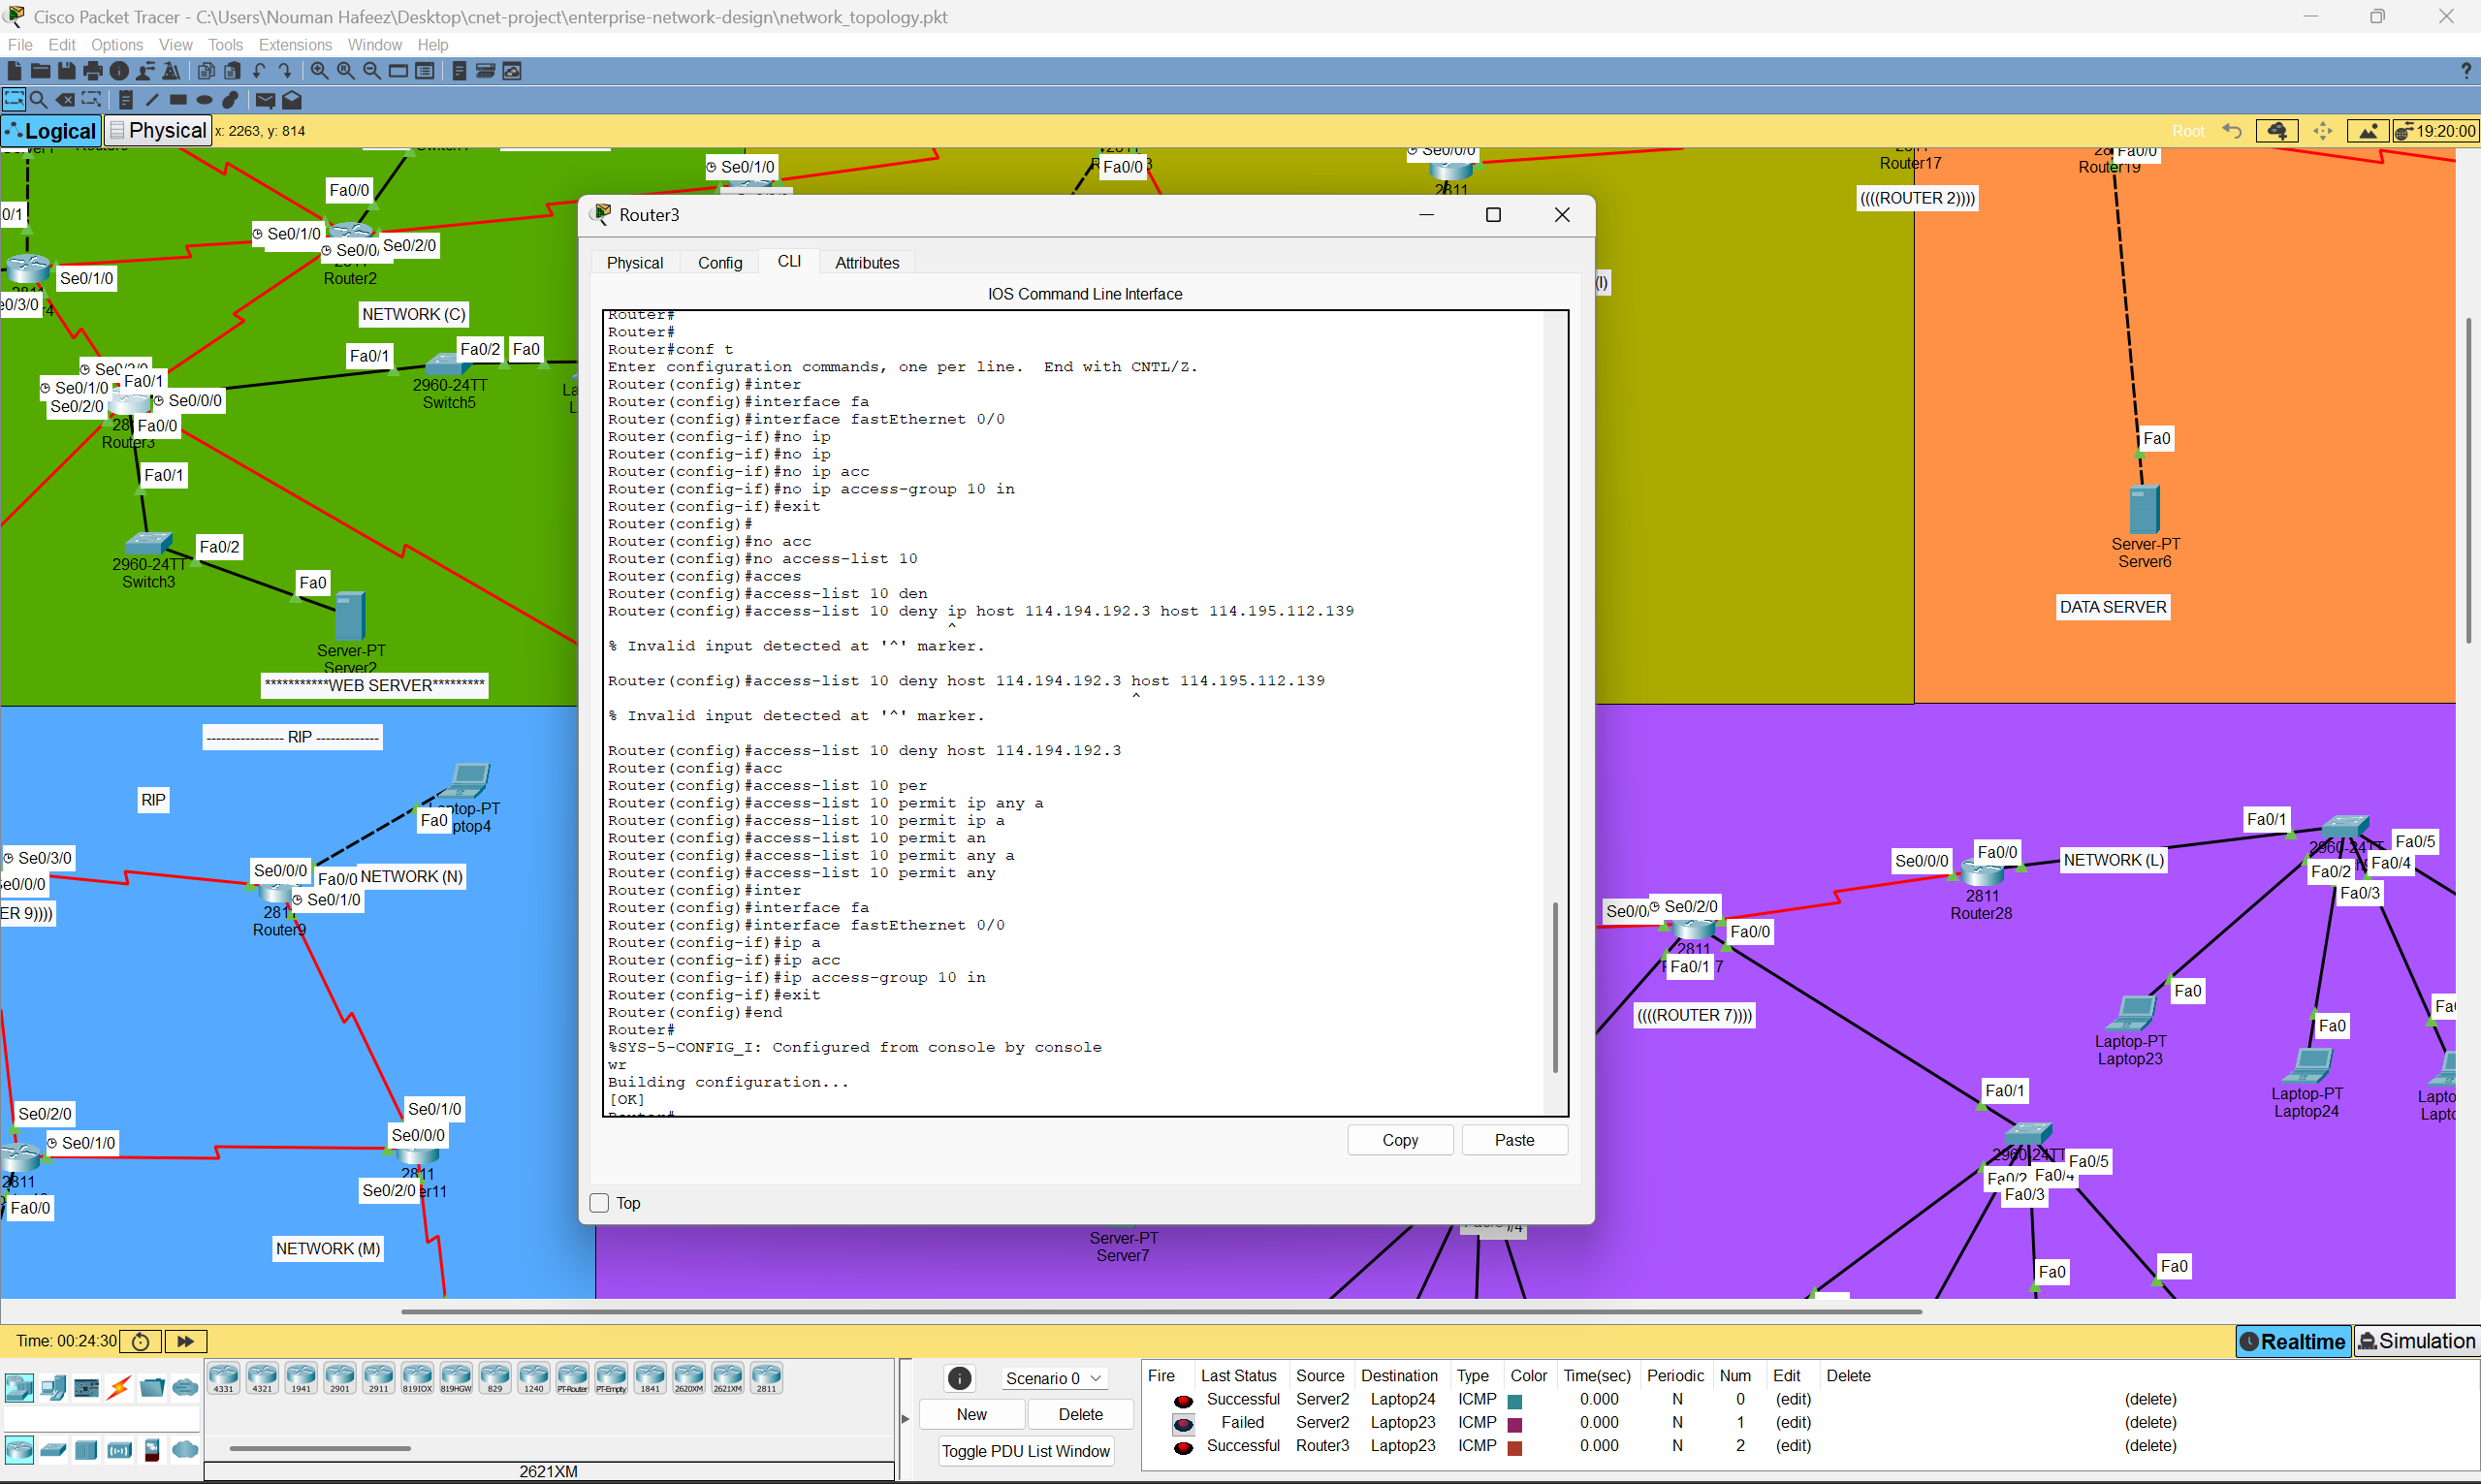
\includegraphics[width=0.9\textwidth]{results/ACL_NETWORK-1_L_WEB-SERVER.png}
    \caption{ACL Configuration for Network 1 - Web Server}
    \label{fig:acl-network1}
\end{figure}

\section{ACL Configuration for Network 2}

Network 2 (Network A) has ACLs configured for TFTP and Data servers. Figure~\ref{fig:acl-network2} shows the ACL configurations.

\begin{figure}[H]
    \centering
    \begin{subfigure}{0.48\textwidth}
        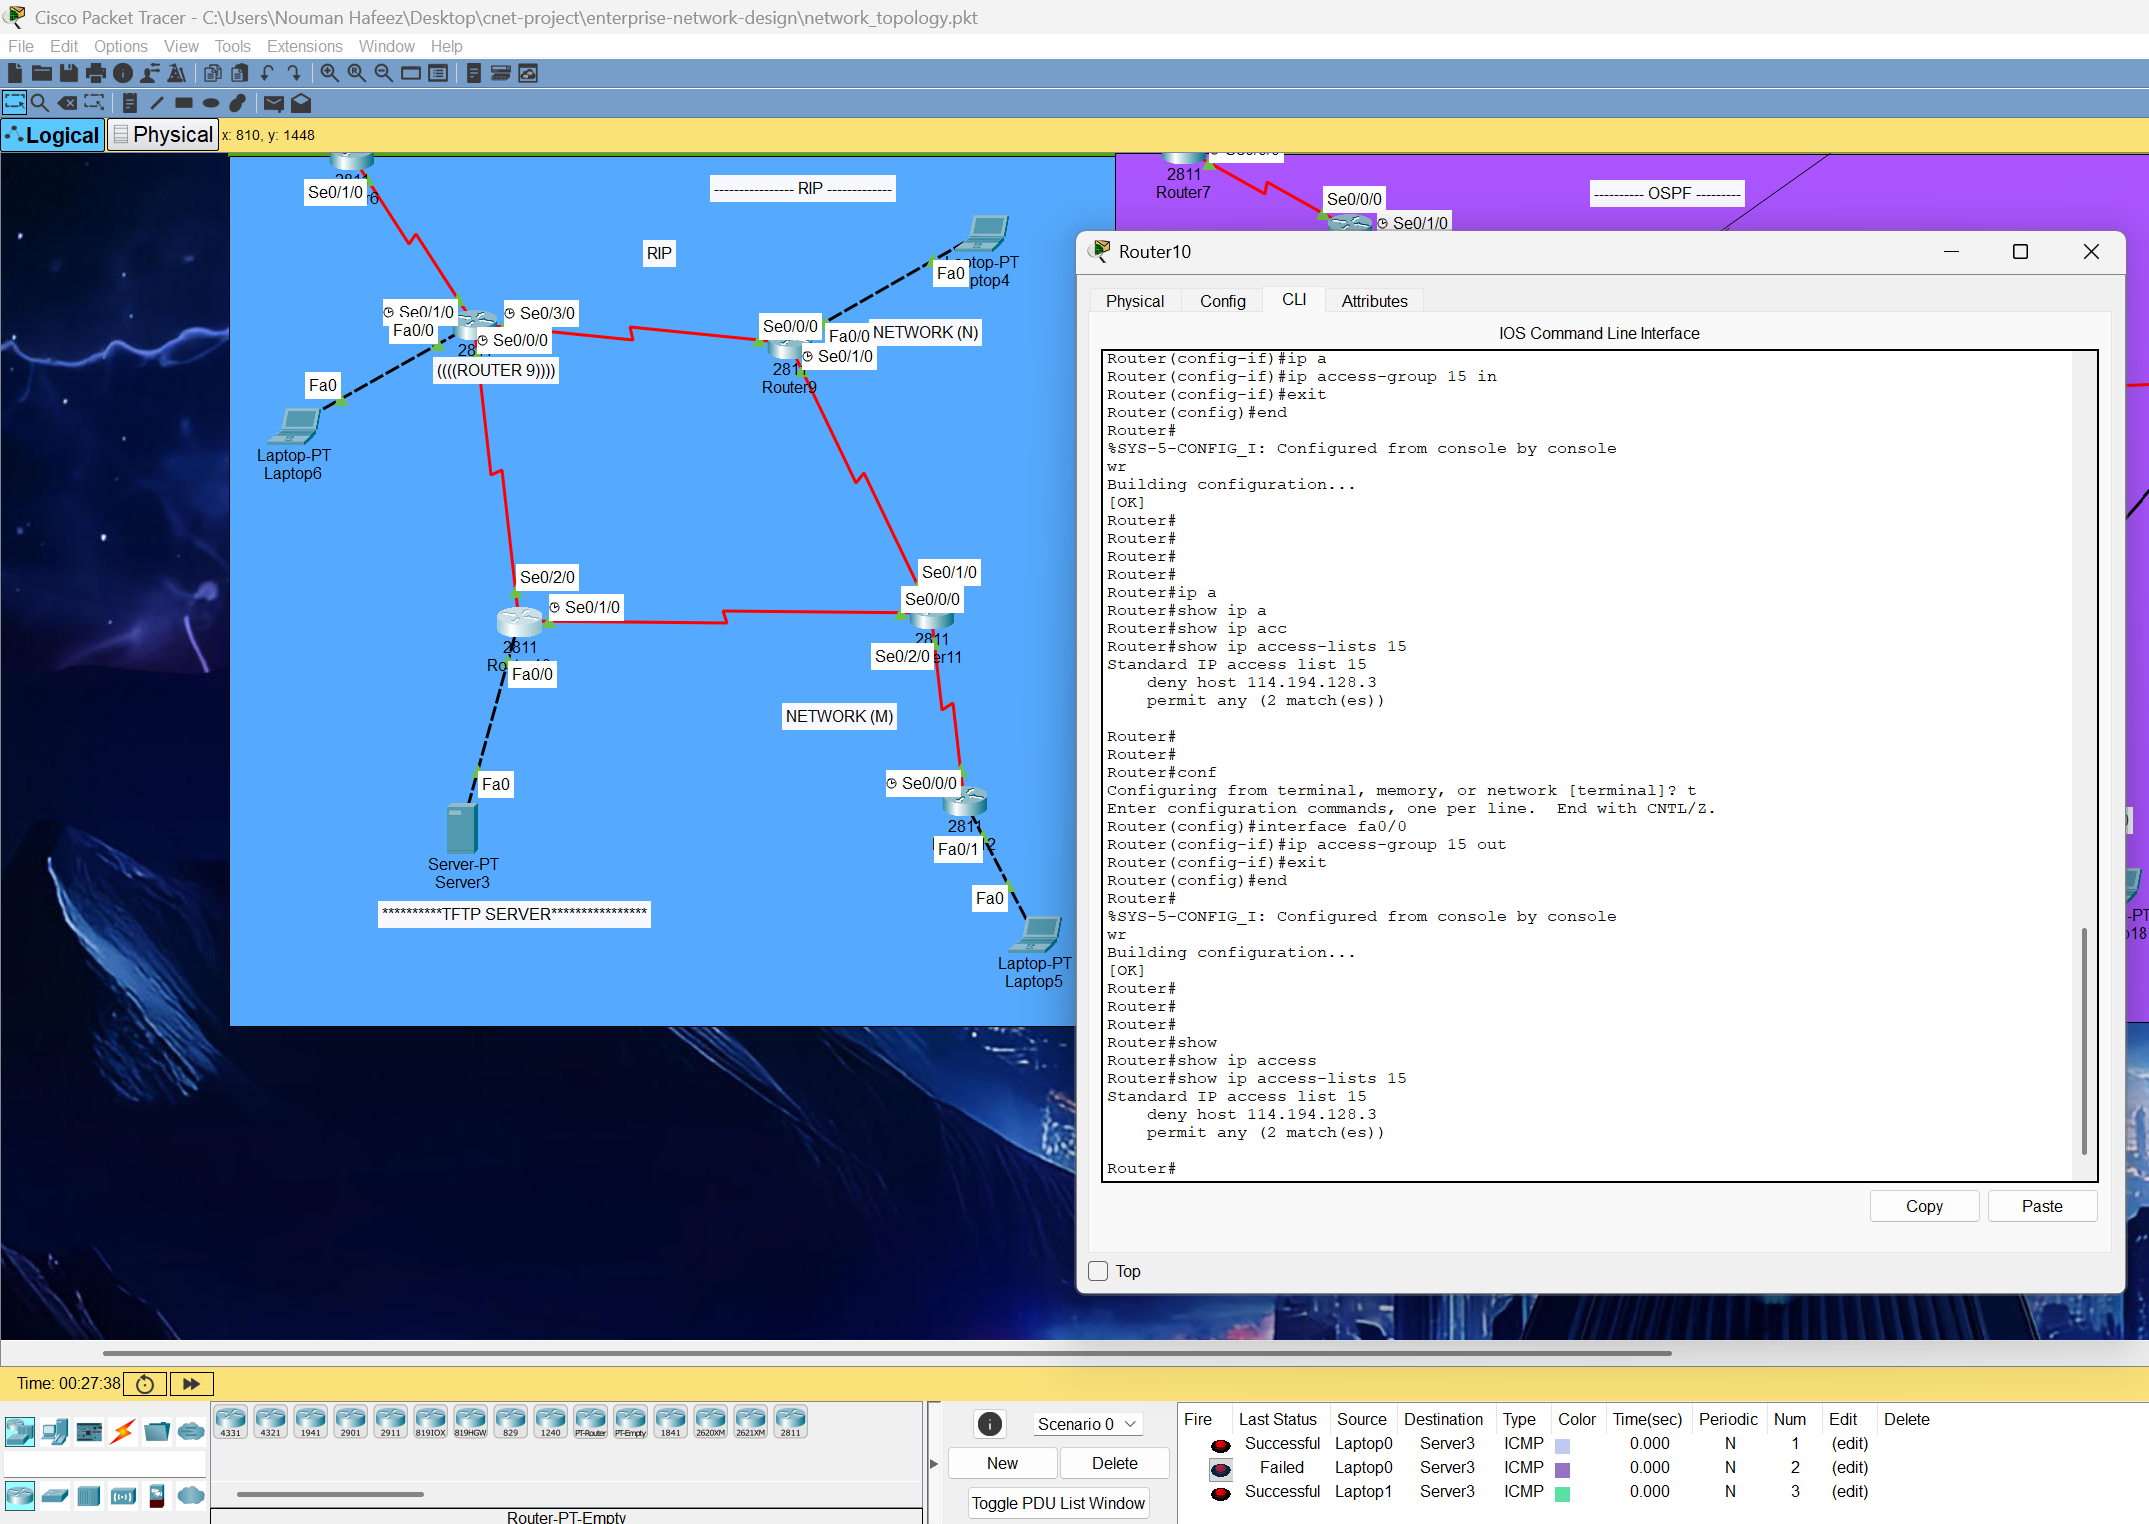
\includegraphics[width=\textwidth]{results/ACL_NETWORK-2_A_TFTP_SERVER.png}
        \caption{ACL for Network 2 - TFTP Server}
    \end{subfigure}
    \hfill
    \begin{subfigure}{0.48\textwidth}
        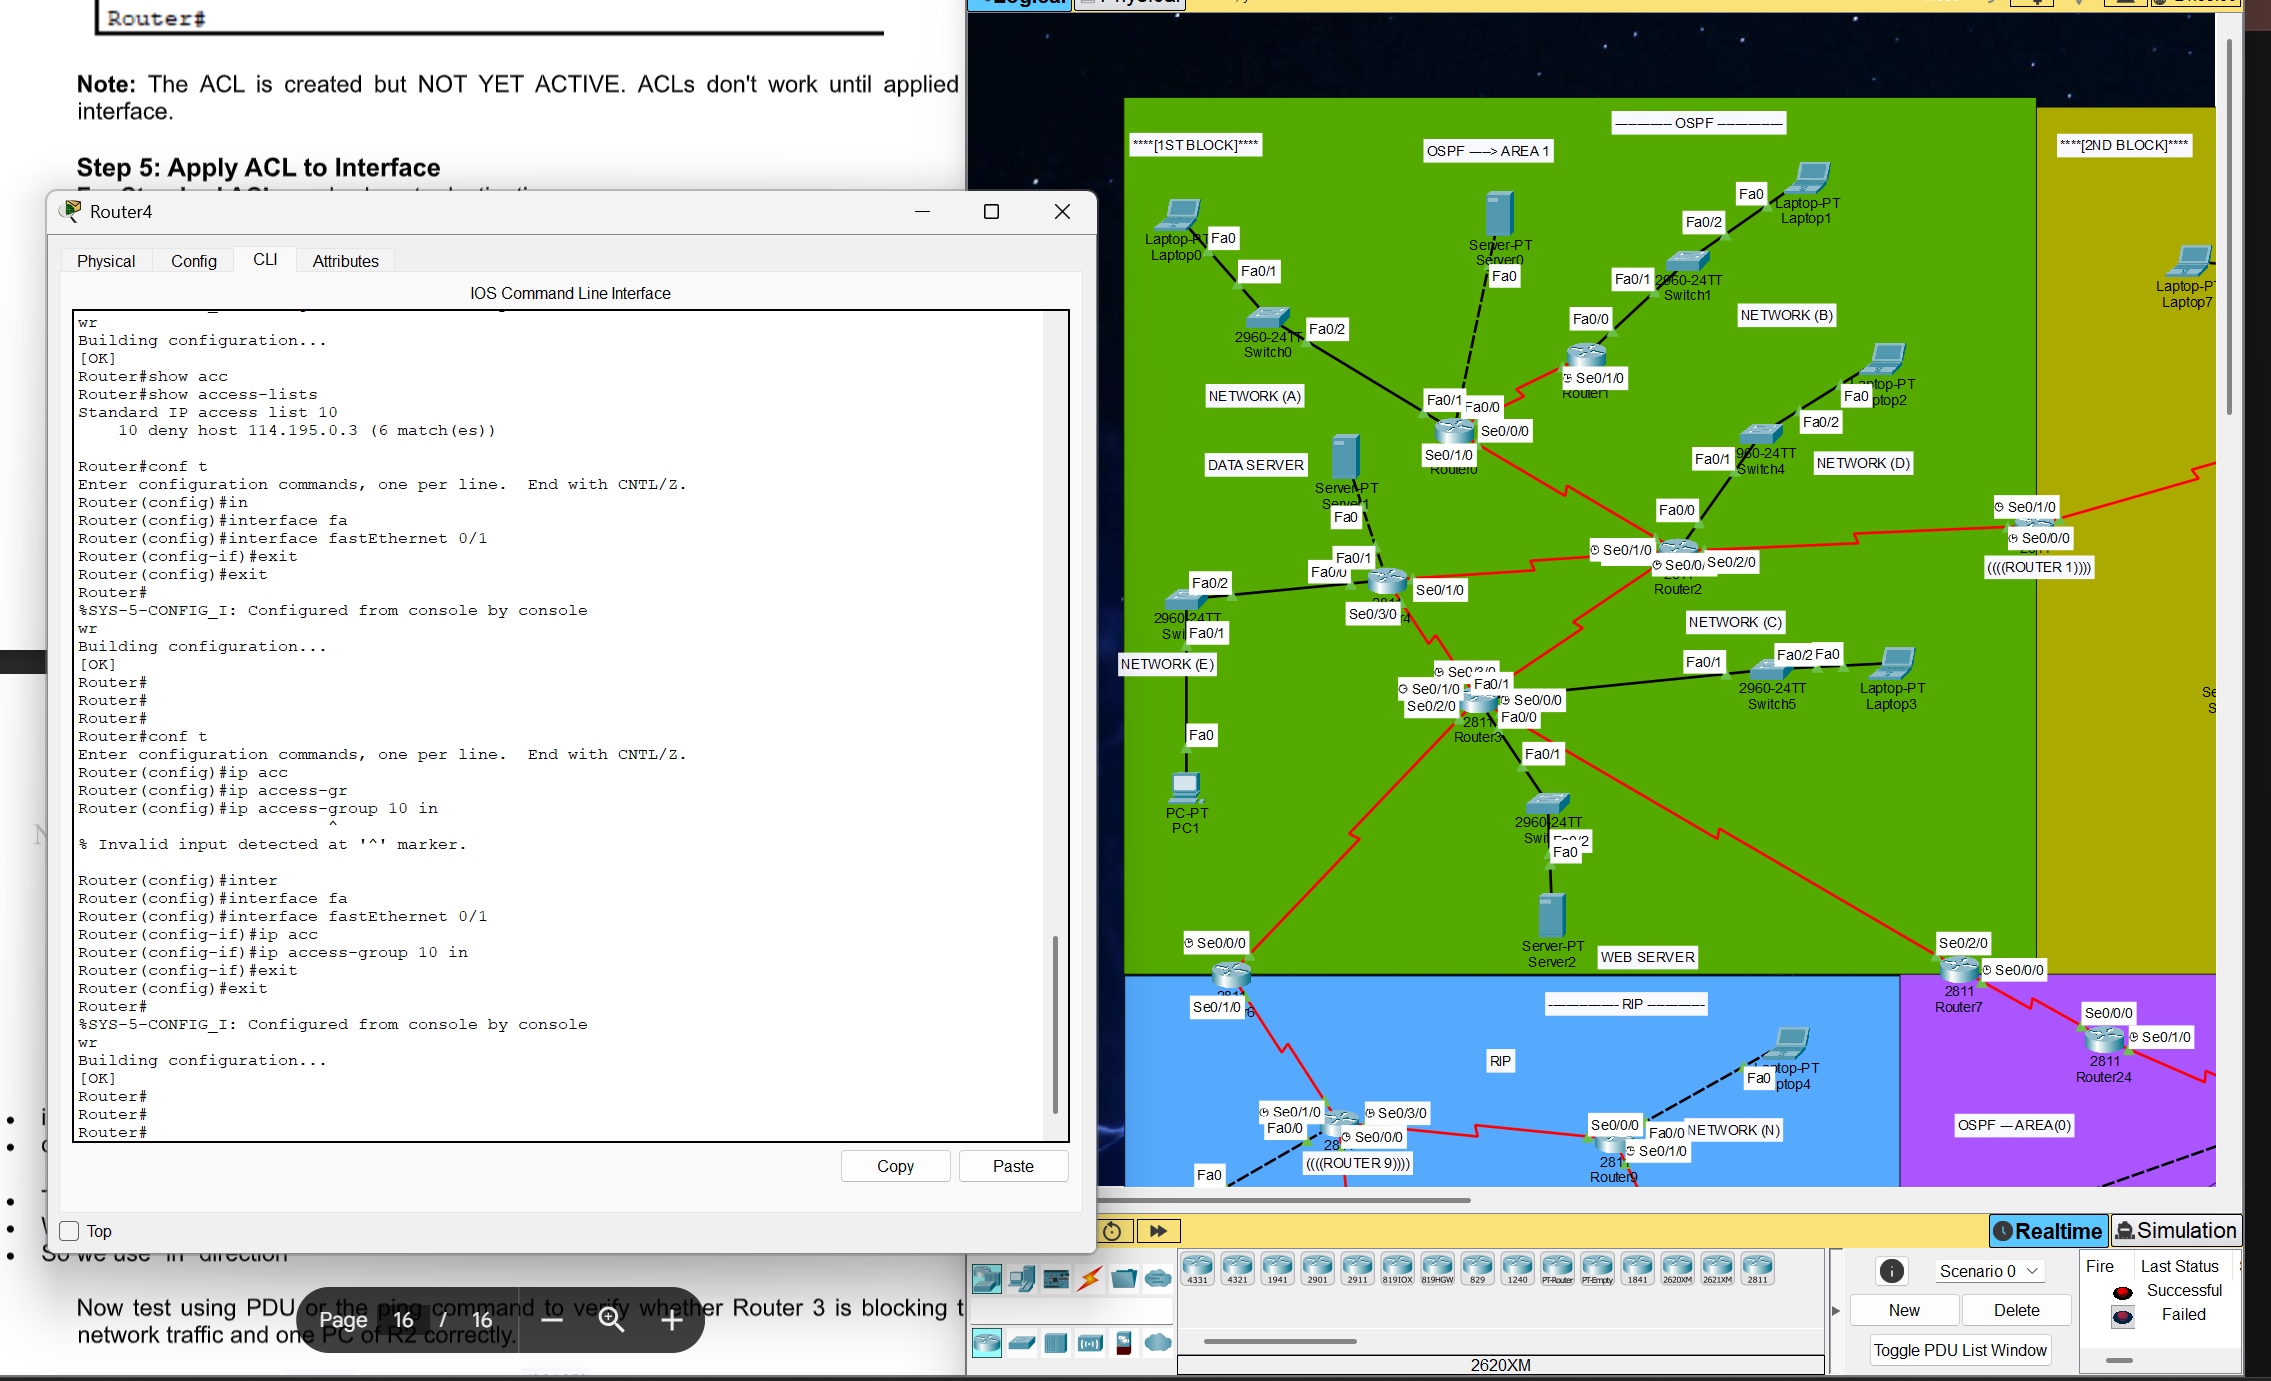
\includegraphics[width=\textwidth]{results/ACL_NETWORK-2_DATA-SERVER.png}
        \caption{ACL for Network 2 - Data Server}
    \end{subfigure}
    \caption{ACL Configuration for Network 2}
    \label{fig:acl-network2}
\end{figure}

\newpage

% Chapter 6: Network Address Translation
\chapter{Network Address Translation (NAT)}

Network Address Translation is configured on Router 10 to enable private network devices to access the internet using a public IP address. Figure~\ref{fig:nat} shows the NAT configuration and verification.

\begin{figure}[H]
    \centering
    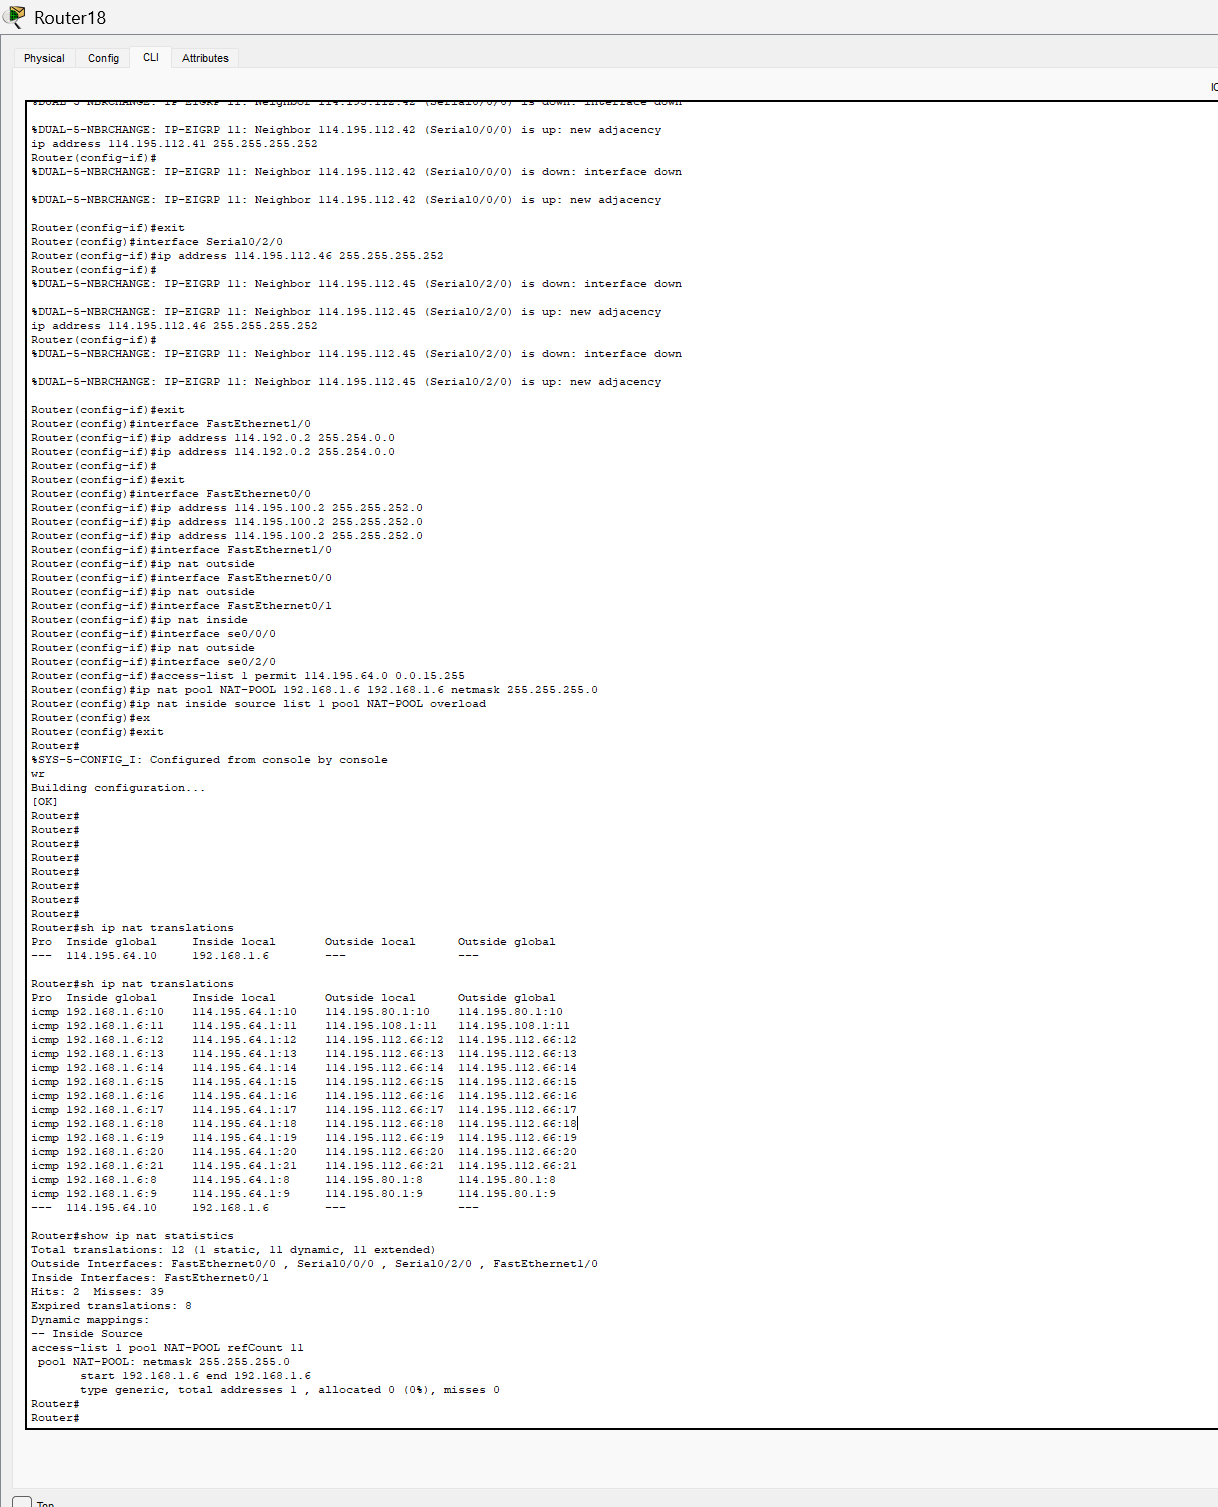
\includegraphics[width=0.9\textwidth]{results/NAT_result.png}
    \caption{NAT Configuration and Verification on Router 10}
    \label{fig:nat}
\end{figure}

\newpage

% Chapter 7: Server Services
\chapter{Server Services Configuration}

This chapter documents the configuration of various server services including TFTP, Web, and Data servers.

\section{TFTP Server Configuration}

The TFTP (Trivial File Transfer Protocol) server is configured at point 10a. Figure~\ref{fig:tftp-server} shows the TFTP server services configuration.

\begin{figure}[H]
    \centering
    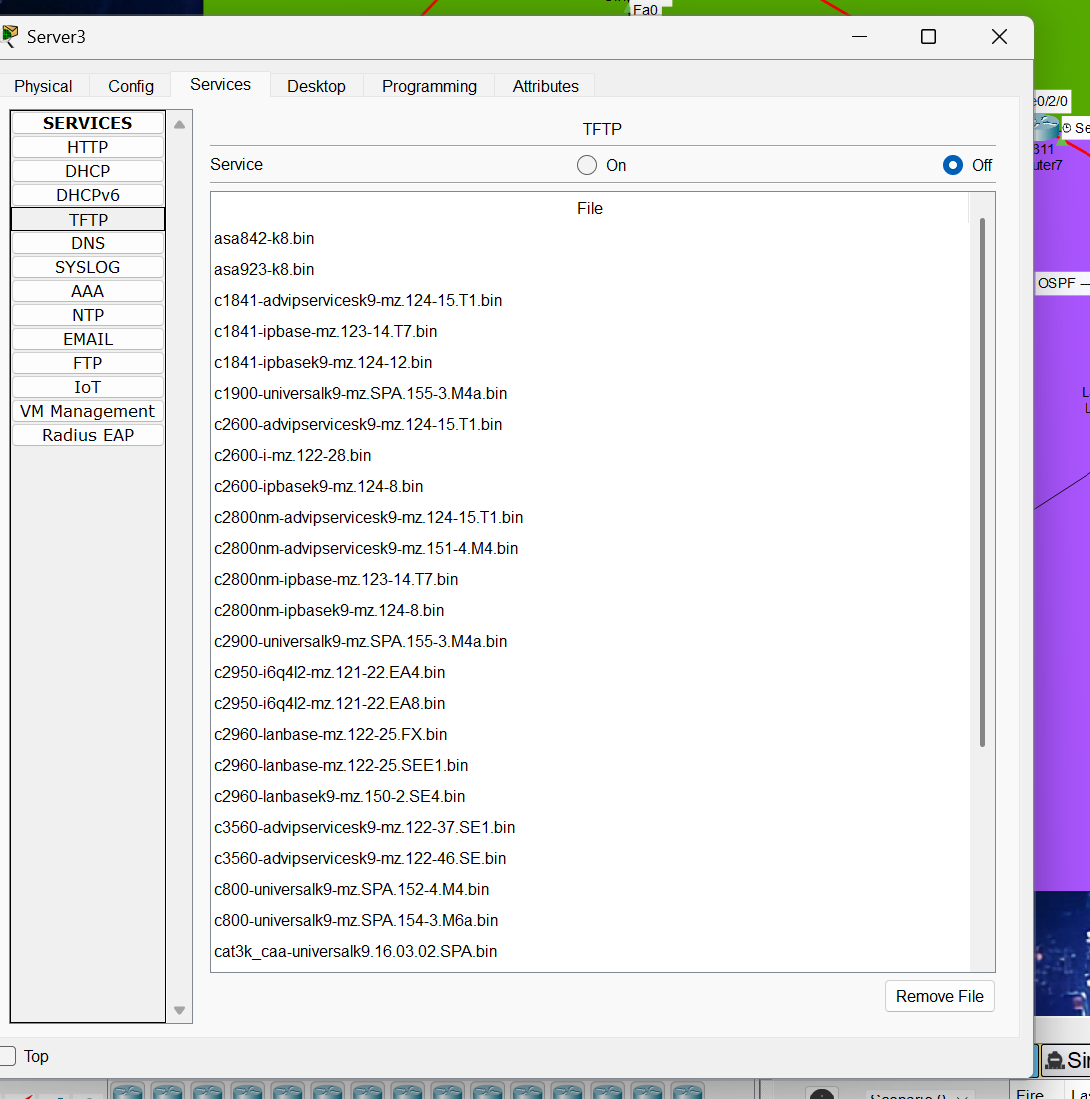
\includegraphics[width=0.9\textwidth]{results/TFTP_SERVER_SERVICES_OFF_POINT_10_a.png}
    \caption{TFTP Server Services Configuration - Point 10a}
    \label{fig:tftp-server}
\end{figure}

\section{Web Server Configuration}

The Web server is configured at point 10b. Figure~\ref{fig:web-server} shows the Web server services configuration.

\begin{figure}[H]
    \centering
    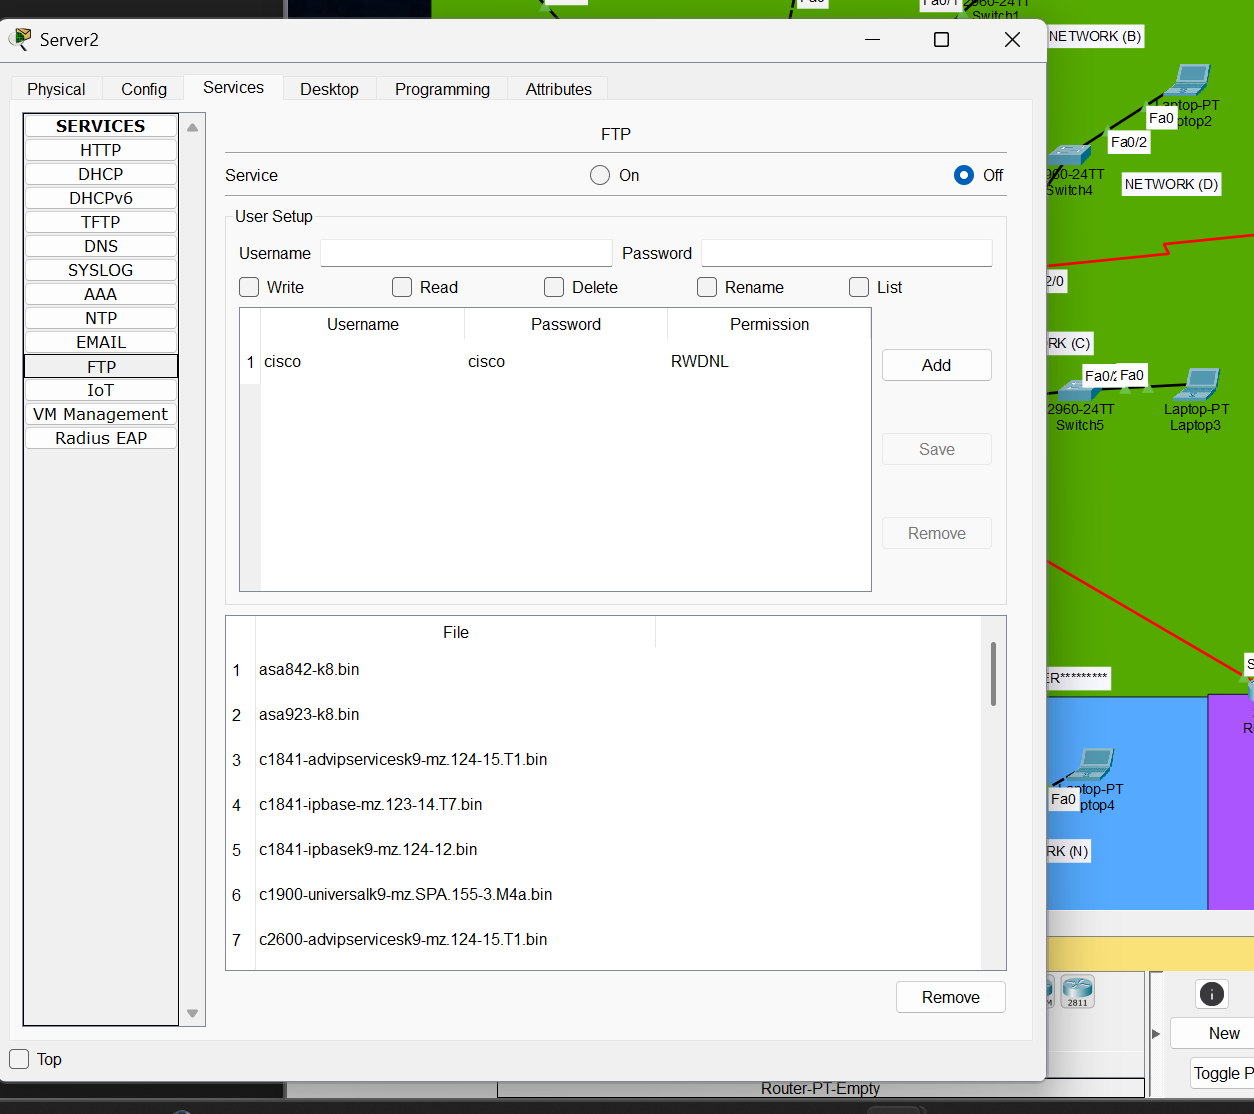
\includegraphics[width=0.9\textwidth]{results/WEB_SERVER_SERVICES_OFF_POINT_10_b.png}
    \caption{Web Server Services Configuration - Point 10b}
    \label{fig:web-server}
\end{figure}

\section{Data Server Configuration}

The Data server is also configured at point 10b. Figure~\ref{fig:data-server} shows the Data server services configuration.

\begin{figure}[H]
    \centering
    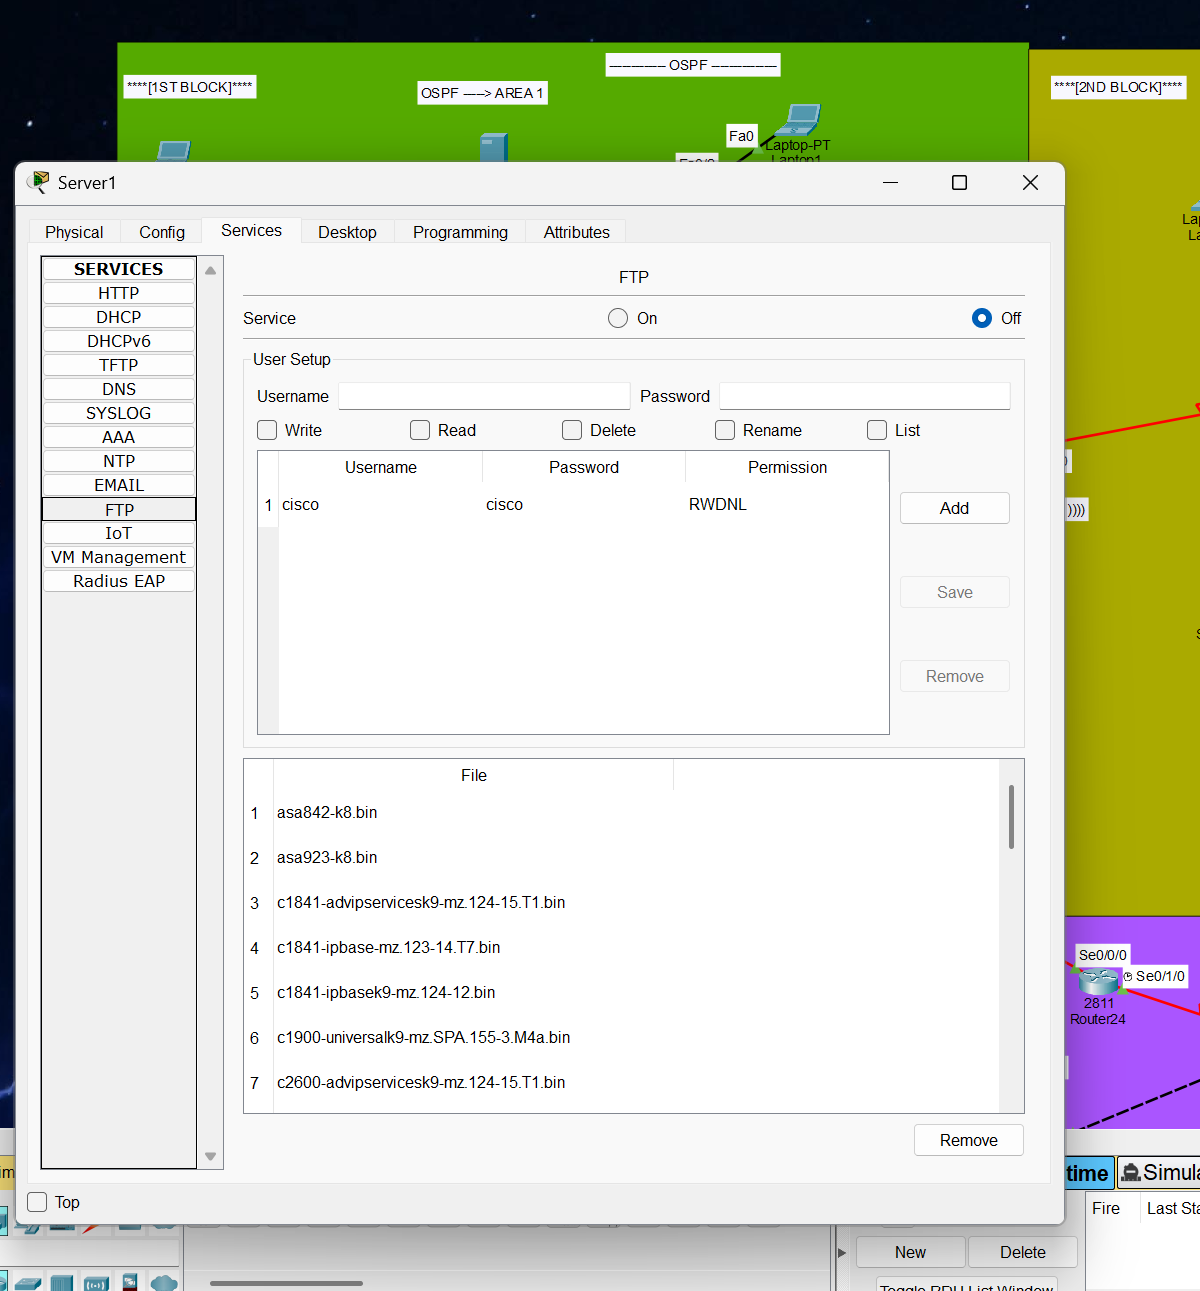
\includegraphics[width=0.9\textwidth]{results/DATA_SERVER_SERVICES_OFF_POINT_10_b.png}
    \caption{Data Server Services Configuration - Point 10b}
    \label{fig:data-server}
\end{figure}

\newpage

% Chapter 8: Web-Based Visualization System
\chapter{Web-Based Visualization System}

A comprehensive web-based visualization system has been developed to provide an interactive interface for viewing the network topology, VLSM configuration, and all project results.

\section{System Overview}

The web visualization system includes:

\begin{itemize}
    \item Interactive VLSM tree visualization with Mermaid.js
    \item Network statistics dashboard with Chart.js
    \item Comprehensive image gallery for all configuration results
    \item Search and filter functionality
    \item Responsive design for multiple devices
    \item Dark theme with modern UI/UX
\end{itemize}

\section{Features}

\subsection{VLSM Tree Visualization}

The system includes an interactive Mermaid.js diagram showing the complete hierarchical structure of all network allocations, including:

\begin{itemize}
    \item Primary networks (A-N) with detailed information
    \item Point-to-point links (29 links)
    \item LAN segments (15 segments)
    \item Future expansion space
\end{itemize}

The diagram supports:
\begin{itemize}
    \item Zoom in/out functionality
    \item Pan and drag navigation
    \item Download as PNG
    \item Custom dark theme matching the site design
\end{itemize}

\subsection{Statistics Dashboard}

Interactive charts display:
\begin{itemize}
    \item Network distribution by category
    \item Address utilization metrics
    \item Subnet size distribution
    \item Host requirements visualization
    \item Efficiency metrics
    \item Address space usage timeline
\end{itemize}

\subsection{Image Gallery}

A comprehensive gallery organizes all project results by category:

\begin{itemize}
    \item Project Topology \& Network Diagrams
    \item VLSM Subnetting Tree Visualizations
    \item Routing Protocol Configuration Results (RIP, OSPF, EIGRP)
    \item Protocol Redistribution Results
    \item DHCP Configuration Results
    \item ACL Configuration
    \item NAT Configuration
    \item Server Services Configuration
\end{itemize}

Each image can be clicked to view in full size with a modal viewer.

\section{Technical Implementation}

The web system is built using:

\begin{itemize}
    \item \textbf{HTML5} for structure
    \item \textbf{CSS3} with modern styling (glassmorphism, gradients, animations)
    \item \textbf{JavaScript} for interactivity
    \item \textbf{Mermaid.js} for diagram rendering
    \item \textbf{Chart.js} for data visualization
\end{itemize}

\section{Access Information}

The web visualization system is located in the \texttt{web/} directory and can be accessed by opening \texttt{index.html} in a modern web browser. The system is fully self-contained and does not require a web server for basic functionality.

\newpage

% Chapter 9: Network Topology
\chapter{Network Topology}

This chapter presents the complete network topology diagrams and configurations.

\section{Project Topology Overview}

Figure~\ref{fig:project-topology} shows the complete project topology.

\begin{figure}[H]
    \centering
    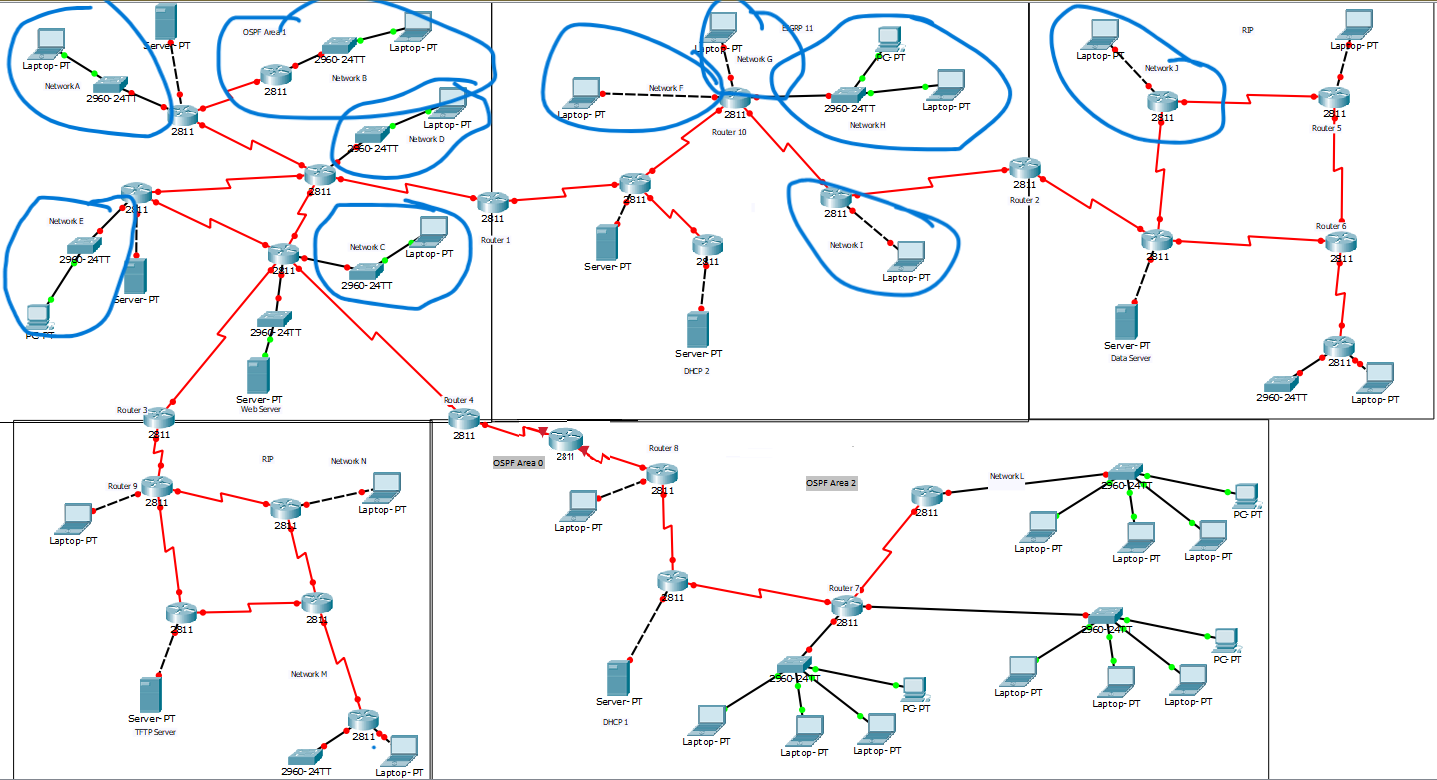
\includegraphics[width=0.95\textwidth]{Project Topology.png}
    \caption{Complete Project Topology}
    \label{fig:project-topology}
\end{figure}

\section{Configured Topology Snapshots}

Figure~\ref{fig:topology-snapshots} shows detailed snapshots of the configured topology.

\begin{figure}[H]
    \centering
    \begin{subfigure}{0.32\textwidth}
        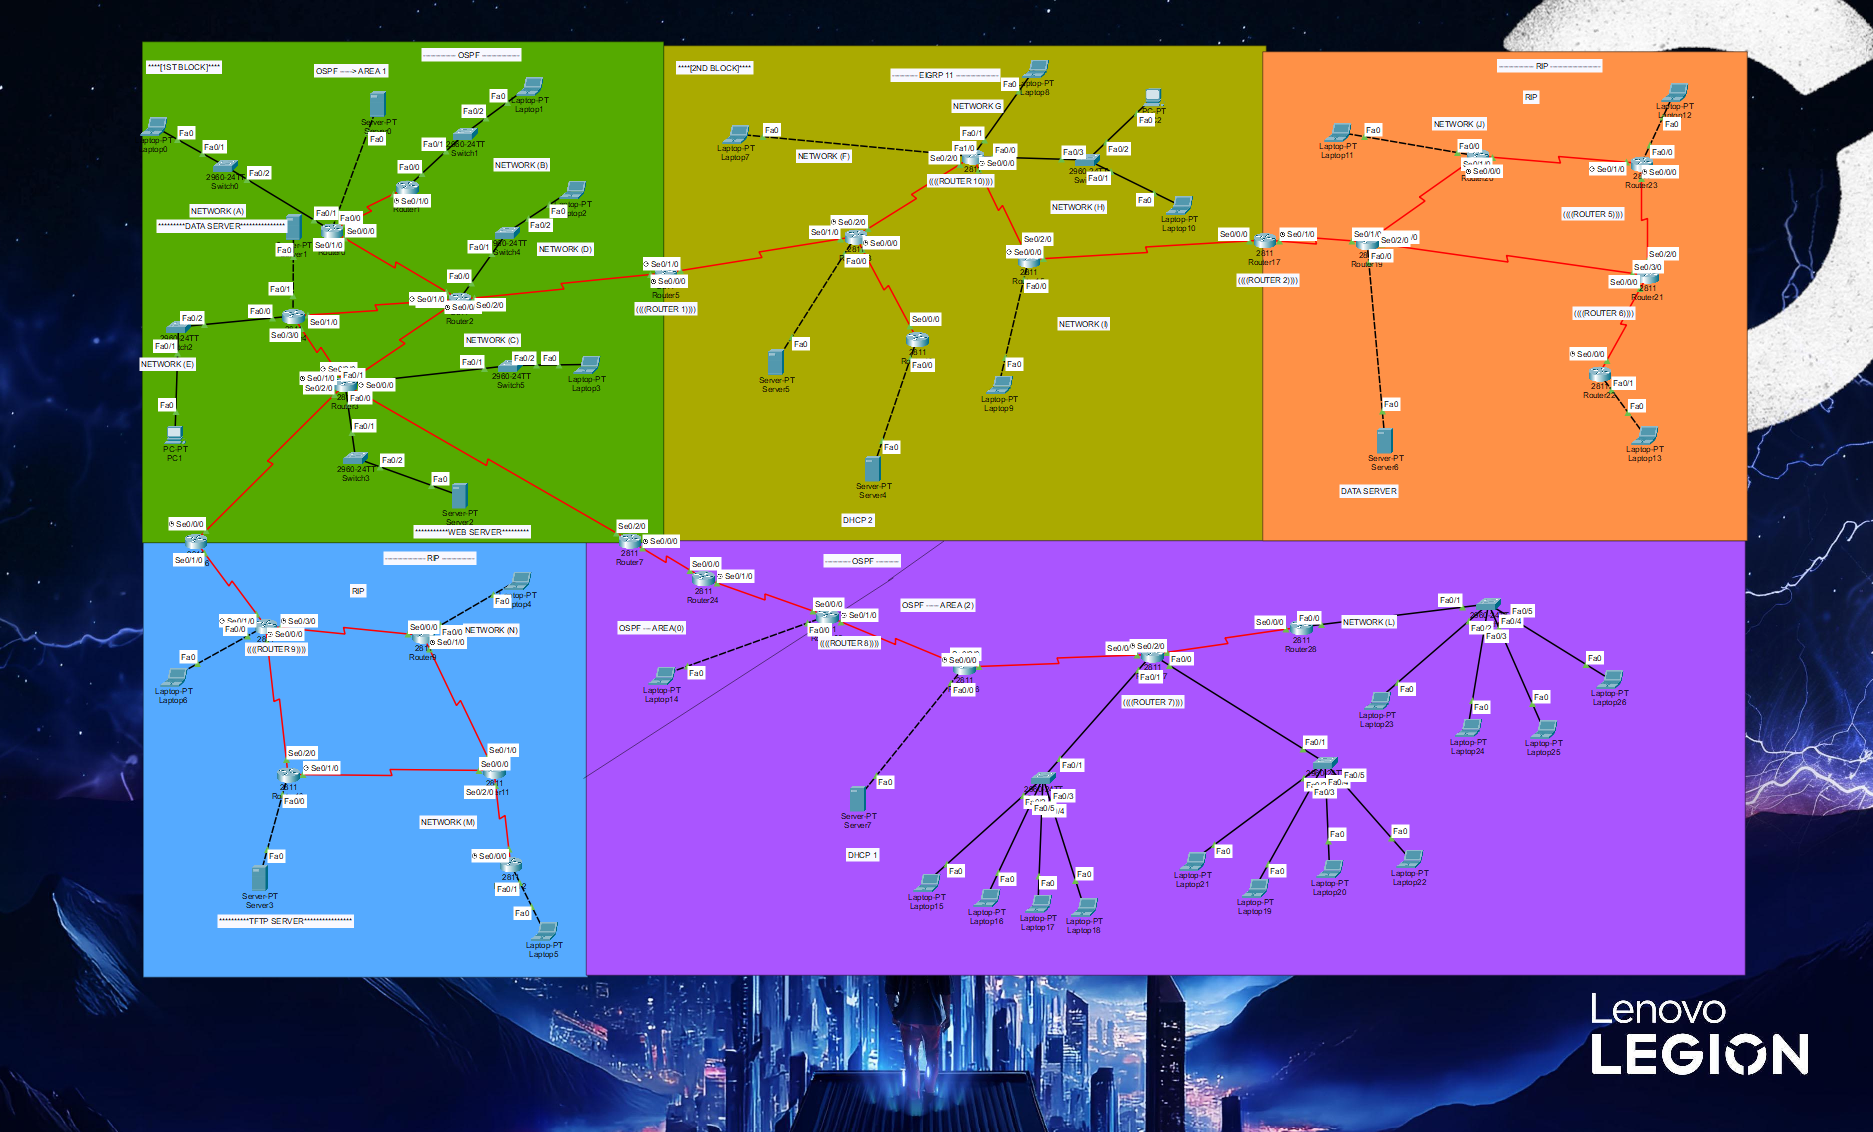
\includegraphics[width=\textwidth]{configured_topology_snapshots/complete_topology.png}
        \caption{Complete Configured Topology}
    \end{subfigure}
    \hfill
    \begin{subfigure}{0.32\textwidth}
        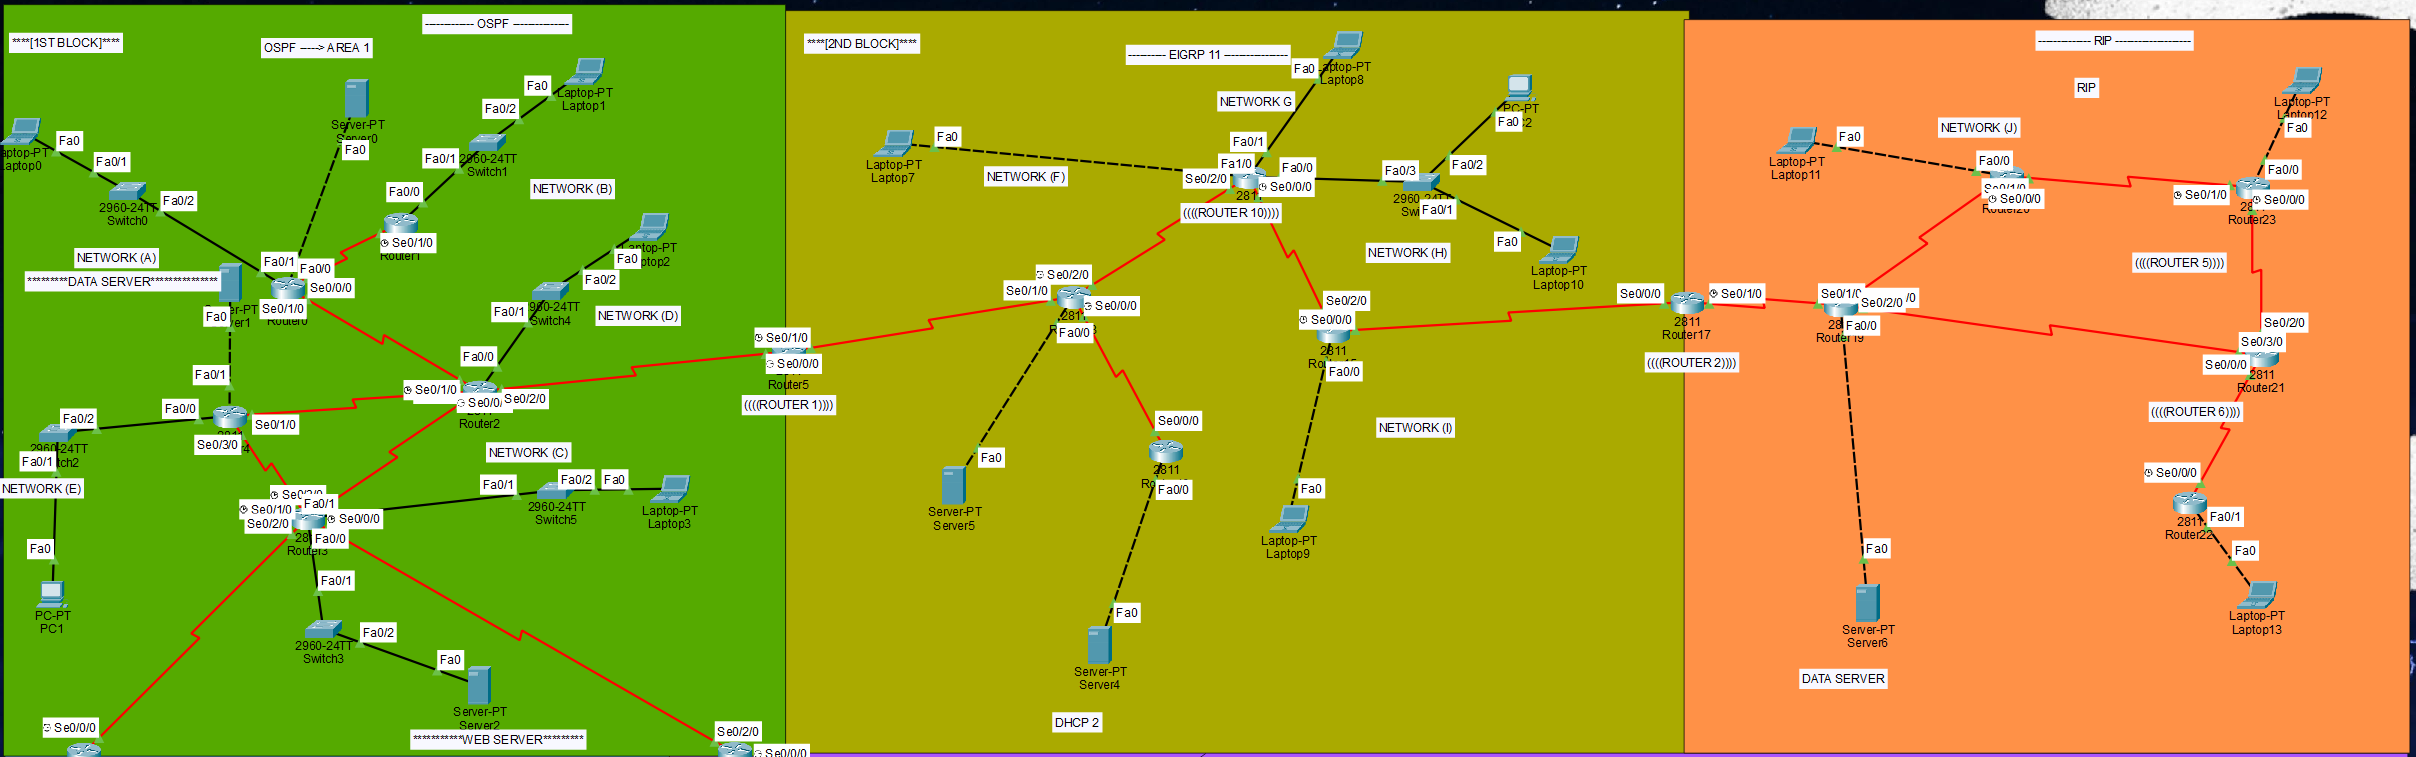
\includegraphics[width=\textwidth]{configured_topology_snapshots/topolgoy_row1.png}
        \caption{Topology Row 1 Configuration}
    \end{subfigure}
    \hfill
    \begin{subfigure}{0.32\textwidth}
        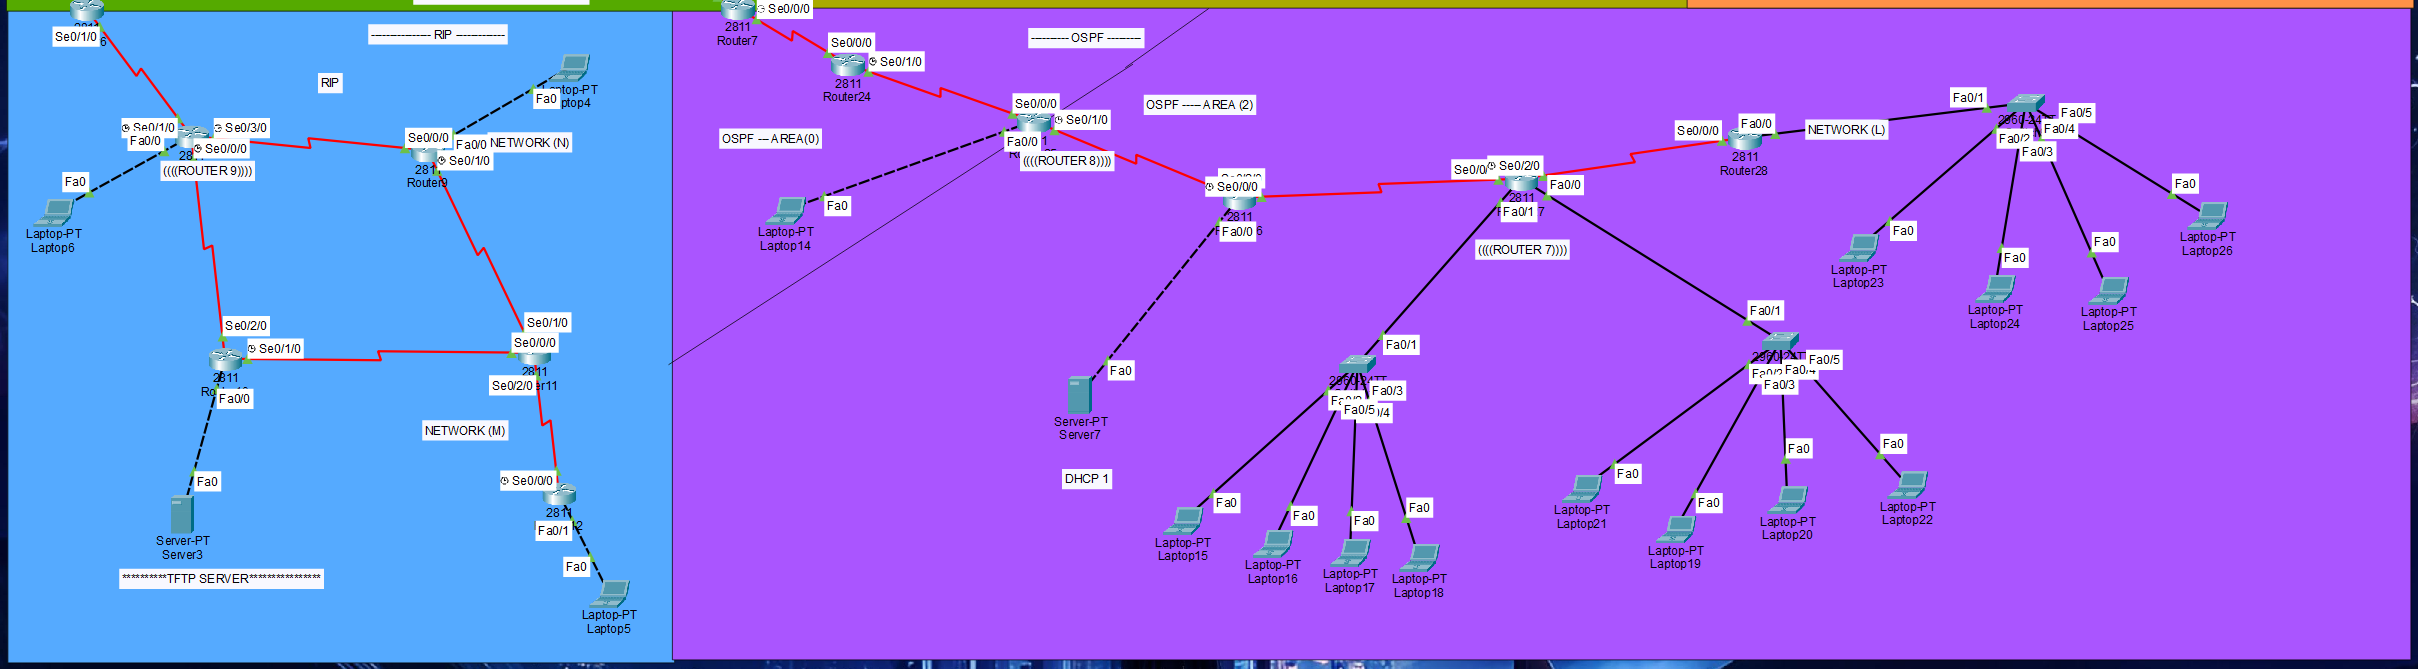
\includegraphics[width=\textwidth]{configured_topology_snapshots/topolgoy_row2.png}
        \caption{Topology Row 2 Configuration}
    \end{subfigure}
    \caption{Configured Topology Snapshots}
    \label{fig:topology-snapshots}
\end{figure}

\section{Other Networks Topology Labels}

Figure~\ref{fig:other-networks} shows the topology with labels for other networks.

\begin{figure}[H]
    \centering
    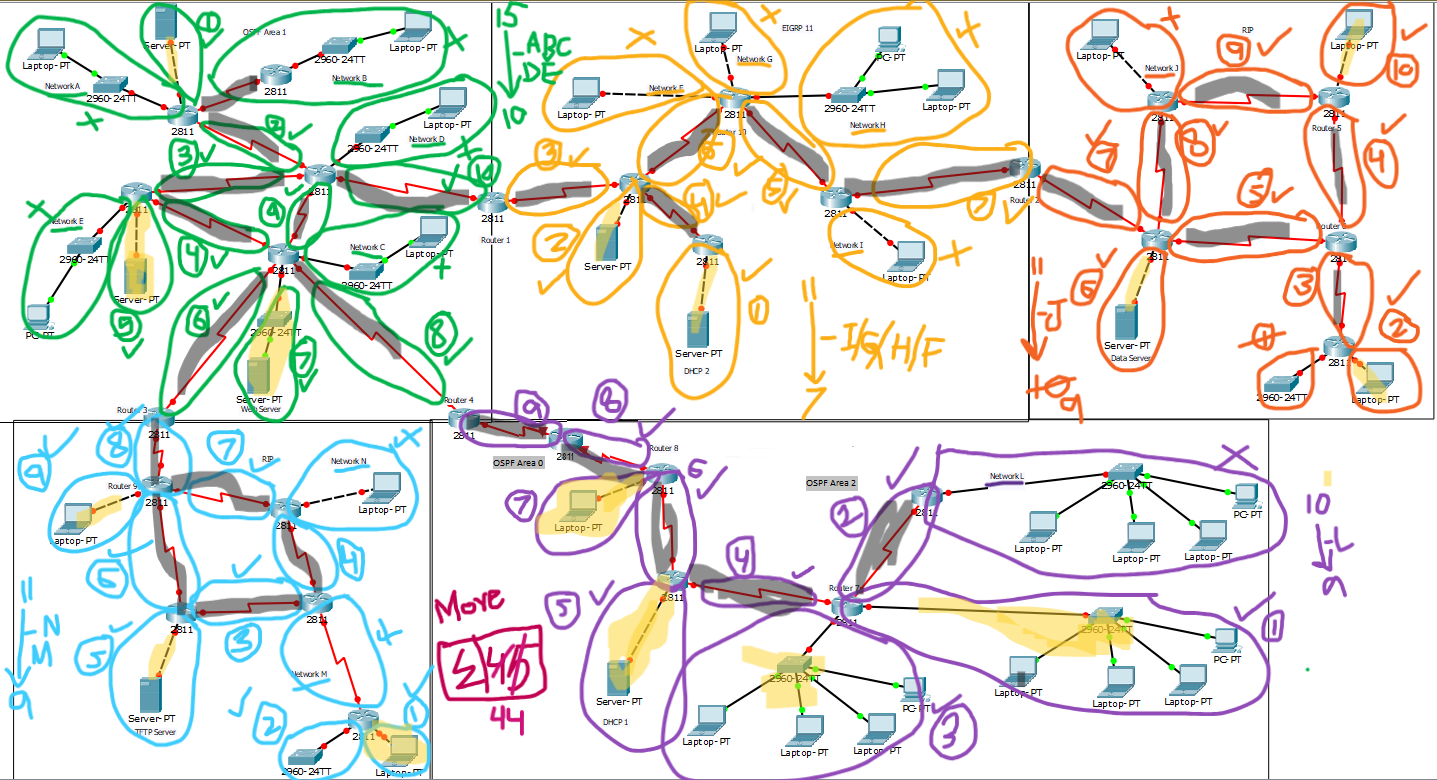
\includegraphics[width=0.9\textwidth]{other_networks_topology_lables.png}
    \caption{Other Networks Topology Labels}
    \label{fig:other-networks}
\end{figure}

\newpage

% Chapter 10: Results and Analysis
\chapter{Results and Analysis}

\section{Configuration Verification}

All network configurations have been successfully implemented and verified. The following sections summarize the key results.

\section{VLSM Allocation Results}

The VLSM subnetting configuration successfully allocated all 13 primary networks within the 114.192.0.0/14 supernet:

\begin{itemize}
    \item \textbf{Total Required Hosts:} 150,978
    \item \textbf{Total Allocated Addresses:} 199,680
    \item \textbf{Total Usable Addresses:} 199,652
    \item \textbf{Address Utilization:} 75.6\%
    \item \textbf{Waste Percentage:} 24.4\%
\end{itemize}

The allocation maintains contiguous addressing, facilitating route summarization and efficient routing table management.

\section{Routing Protocol Results}

\subsection{RIP Configuration}

RIP has been successfully configured and verified across multiple network segments. Routing tables show proper route propagation and convergence.

\subsection{OSPF Configuration}

OSPF has been configured with multiple areas (Area 0, Area 1, Area 2) for hierarchical routing. All areas are properly connected and routing information is being exchanged correctly.

\subsection{EIGRP Configuration}

EIGRP has been configured and is functioning correctly. The protocol is successfully learning and advertising routes within its autonomous system.

\subsection{Protocol Redistribution}

Route redistribution has been successfully configured between:
\begin{itemize}
    \item RIP and EIGRP
    \item OSPF Area 1 and RIP
    \item OSPF Area 1 and EIGRP
    \item OSPF inter-area redistribution (Area 0, Area 1, Area 2)
    \item OSPF and EIGRP
\end{itemize}

All redistribution points are verified and routes are being properly exchanged.

\section{DHCP Configuration Results}

Both DHCP servers have been successfully configured:
\begin{itemize}
    \item DHCP Server 1: Configured for Row 2 networks with TFTP option
    \item DHCP Server 2: Configured for Row 1 networks
\end{itemize}

DHCP pools are properly configured and verified through show commands.

\section{ACL Configuration Results}

Access Control Lists have been successfully implemented:
\begin{itemize}
    \item Network 1 (Network L): ACL configured for Web Server access control
    \item Network 2 (Network A): ACLs configured for TFTP and Data servers
\end{itemize}

All ACLs are properly applied and filtering traffic as intended.

\section{NAT Configuration Results}

Network Address Translation has been successfully configured on Router 10. The NAT translation table shows proper mapping between private and public IP addresses, enabling internet connectivity for private network devices.

\section{Server Services Results}

All server services have been successfully configured:
\begin{itemize}
    \item TFTP Server: Operational at point 10a
    \item Web Server: Operational at point 10b
    \item Data Server: Operational at point 10b
\end{itemize}

All services are accessible and functioning correctly.

\section{Web Visualization System Results}

The web-based visualization system has been successfully developed and includes:
\begin{itemize}
    \item Interactive Mermaid.js VLSM tree diagram
    \item Comprehensive statistics dashboard with 6 different charts
    \item Image gallery with 43+ configuration result images
    \item Fully responsive design
    \item Modern dark theme UI
\end{itemize}

The system provides an intuitive interface for viewing all project components and results.

\newpage

% Chapter 11: Conclusion
\chapter{Conclusion}

\section{Project Summary}

This enterprise network design project successfully demonstrates the implementation of advanced networking concepts including VLSM subnetting, multiple routing protocols, DHCP, ACLs, NAT, and server services. The project successfully accommodates all network requirements while maintaining efficient address space utilization.

\section{Key Achievements}

\begin{itemize}
    \item Successfully allocated all 13 primary networks (A through N) with varying host requirements (835 to 83,492 hosts)
    \item Implemented efficient VLSM subnetting with 75.6\% address utilization
    \item Configured and verified three routing protocols (RIP, OSPF, EIGRP) with proper redistribution
    \item Successfully implemented DHCP services for automatic IP address allocation
    \item Configured Access Control Lists for network security
    \item Implemented Network Address Translation for internet connectivity
    \item Configured multiple server services (TFTP, Web, Data servers)
    \item Developed a comprehensive web-based visualization system
\end{itemize}

\section{Technical Highlights}

\subsection{VLSM Efficiency}

The VLSM implementation achieved:
\begin{itemize}
    \item Efficient address allocation minimizing wastage
    \item Contiguous addressing for route summarization
    \item Proper allocation of 29 P2P links and 15 LAN segments
    \item Reserved space for future expansion
\end{itemize}

\subsection{Routing Protocol Integration}

The multi-protocol routing environment successfully integrates:
\begin{itemize}
    \item RIP for distance-vector routing
    \item OSPF for link-state routing with multiple areas
    \item EIGRP for hybrid routing
    \item Comprehensive route redistribution between all protocols
\end{itemize}

\subsection{Network Services}

All network services have been successfully implemented:
\begin{itemize}
    \item DHCP for automatic IP configuration
    \item ACLs for traffic filtering and security
    \item NAT for internet connectivity
    \item Server services for network applications
\end{itemize}

\section{Web Visualization System}

The web-based visualization system provides:
\begin{itemize}
    \item Interactive VLSM tree diagram with zoom and pan capabilities
    \item Comprehensive statistics and analytics
    \item Organized image gallery for all configuration results
    \item Modern, responsive user interface
\end{itemize}

\section{Future Enhancements}

Potential future enhancements include:
\begin{itemize}
    \item Integration of IPv6 addressing
    \item Implementation of advanced security features (firewalls, VPNs)
    \item Network monitoring and management tools
    \item Automated configuration backup and restoration
    \item Enhanced web visualization with real-time network status
\end{itemize}

\section{Final Remarks}

This project successfully demonstrates comprehensive understanding and practical implementation of enterprise network design principles. All objectives have been achieved, and the network is fully functional with proper configuration verification. The project showcases efficient IP address management, multi-protocol routing, and modern web-based visualization techniques.

The implementation follows industry best practices and standards, ensuring scalability, maintainability, and security. The web visualization system provides an excellent tool for network documentation and presentation.

\newpage

% Appendices
\appendix

\chapter{Additional Configuration Details}

\section{Complete Network Allocation Table}

The complete network allocation table includes all primary networks, P2P links, and LAN segments as documented in Chapter 2.

\section{Configuration Files}

All configuration files and Packet Tracer topology file are available in the project directory:
\begin{itemize}
    \item \texttt{network\_topology.pkt} - Packet Tracer topology file
    \item \texttt{web/} - Web visualization system
    \item \texttt{results/} - All configuration result screenshots
    \item \texttt{documentation/} - Additional documentation PDFs
\end{itemize}

\chapter{References}

\begin{itemize}
    \item Cisco Systems. (2023). \textit{Cisco IOS Configuration Guide}
    \item RFC 1918 - Address Allocation for Private Internets
    \item RFC 2328 - OSPF Version 2
    \item RFC 2453 - RIP Version 2
    \item RFC 2131 - Dynamic Host Configuration Protocol
    \item Mermaid.js Documentation: \url{https://mermaid.js.org/}
    \item Chart.js Documentation: \url{https://www.chartjs.org/}
\end{itemize}

\end{document}

